%--------------------------------------------------------------------%
%
% Berkas utama templat LaTeX.
%
% author Petra Barus, Peb Ruswono Aryan, Faris Rizki Ekananda
%
%--------------------------------------------------------------------%
%
% Berkas ini berisi struktur utama dokumen LaTeX yang akan dibuat.
%
%--------------------------------------------------------------------%

\documentclass[bahasa, 12pt, a4paper, onecolumn, oneside, final]{report}

%-------------------------------------------------------------------%
%
% Konfigurasi dokumen LaTeX untuk laporan tesis IF ITB
%
% @author Petra Novandi
%
%-------------------------------------------------------------------%
%
% Berkas asli berasal dari Steven Lolong
%
%-------------------------------------------------------------------%

% Ukuran kertas
\special{papersize=210mm,297mm}

% Setting margin
\usepackage[top=2cm,bottom=2cm,left=4cm,right=3cm]{geometry}

% Math package
\usepackage{mathptmx}

% 4th Sectioning
\newcommand{\subsubsubsection}[1]{\paragraph{#1}\mbox{}\\}
\usepackage{titlesec}

\titleformat{\subsubsubsection}
{\normalfont\normalsize\bfseries}{\theparagraph}{1em}{}
\titlespacing*{\subsubsubsection}
{0pt}{3.25ex plus 1ex minus .2ex}{1.5ex plus .2ex}

% Judul bahasa Indonesia
\usepackage[bahasa]{babel}

% Format citation
\usepackage[utf8]{inputenc}
\usepackage[style=apa,backend=biber]{biblatex}
\usepackage{longtable}
\usepackage{graphicx}
\usepackage{subfig}
\usepackage{titling}
\usepackage{booktabs}
\usepackage{tabularx}
\usepackage{blindtext}
\usepackage{sectsty}
\usepackage{chngcntr}
\usepackage{etoolbox}
\usepackage{array}
\usepackage[hidelinks]{hyperref}       % Package untuk link di daftar isi. Ubah jadi \usepackage[hidelinks]{hyperref} apabila ingin menghilangkan kotak merah disekitar link
\usepackage{titlesec}       % Package Format judul
\usepackage{titletoc}       % Package Format judul di toc
\usepackage{tocbibind}      % Package untuk masukkan toc, lot, lof ke Daftar Isi
\usepackage{scrwfile}       % Package untuk membuat Daftar Lampiran dari toc
\usepackage{parskip}
\usepackage{afterpage}
\usepackage{relsize}
\usepackage{xcolor, colortbl}
\usepackage{setspace}
\usepackage{listings}

\graphicspath{{resources/}}   % letak direktori penyimpanan gambar

% Setting daftar lampiran
\newcommand*{\lopname}{DAFTAR LAMPIRAN}
\TOCclone[\lopname]{toc}{atoc}
\addtocontents{atoc}{\protect\value{tocdepth}=-1}
\newcommand\listofappendices{
  \cleardoublepage
  \phantomsection
  \listofatoc
  \addcontentsline{toc}{chapter}{\lopname}
}

\newcommand*\savedtocdepth{}
\AtBeginDocument{%
  \edef\savedtocdepth{\the\value{tocdepth}}%
}

\let\originalappendix\appendix
\renewcommand\appendix{%
  \originalappendix
  \cleardoublepage
  \addtocontents{toc}{\protect\value{tocdepth}=-1}%
  \addtocontents{atoc}{\protect\value{tocdepth}=\savedtocdepth}%

  \titlecontents{chapter}
    [0pt]
    {\bfseries}
    {Lampiran \thecontentslabel.\quad}
    {}
    {\hfill\contentspage}

  \titleformat{\chapter}[block]
    {\bfseries}
    {\chaptertitlename\ \thechapter.\quad}{0pt}
    {\bfseries}
}

% Hilangkan titik pada toc
\makeatletter
\renewcommand{\@dotsep}{1} 
\makeatother

% Setel title pada chapter-chapter di toc, lof, lot
\titlecontents{chapter}
  [0pt]
  {\bfseries}
  {\MakeUppercase{Bab} \thecontentslabel\quad\uppercase}
  {}
  {\mdseries\titlerule*[0.35em]{.}\bfseries\contentspage}
\titlecontents{figure}
  [0pt]
  {}
  {Gambar \thecontentslabel.\quad}
  {}
  {\mdseries\titlerule*[0.35em]{.}\bfseries\contentspage}
\titlecontents{table}
  [0pt]
  {}
  {Tabel \thecontentslabel.\quad}
  {}
  {\mdseries\titlerule*[0.35em]{.}\bfseries\contentspage}

% Masukin Daftar Pustaka ke toc
\let\originalprintbibliography\printbibliography
\renewcommand\printbibliography{%
  \phantomsection
  \cleardoublepage
  \originalprintbibliography
  \addcontentsline{toc}{chapter}{\bibname}
}

% Line satu setengah spasi
\renewcommand{\baselinestretch}{1.5}

% Setting judul
\chapterfont{\centering \large}
\titleformat{\chapter}[display]
  {\Large\centering\bfseries}
  {\chaptertitlename\ \thechapter}{0pt}
    {\Large\bfseries\uppercase}

% Setting nomor pada subbsubsubbab
\setcounter{secnumdepth}{4}

\makeatletter

\makeatother

% Counter untuk figure dan table.
\counterwithin{figure}{chapter}
\counterwithin{table}{chapter}

% Define blank page
\newcommand*{\blankpage}{\afterpage{\null\newpage}}

% Translate autoref into Indonesian
\renewcommand*{\equationautorefname}{Persamaan}%
\renewcommand*{\footnoteautorefname}{catatan kaki}%
\renewcommand*{\itemautorefname}{item}%
\renewcommand*{\figureautorefname}{Gambar}%
\renewcommand*{\tableautorefname}{Tabel}%
\renewcommand*{\partautorefname}{Bagian}%
\renewcommand*{\appendixautorefname}{Lampiran}%
\renewcommand*{\chapterautorefname}{Bab}%
\renewcommand*{\sectionautorefname}{Subbab}%
\renewcommand*{\subsectionautorefname}{Subsubbab}%
\renewcommand*{\subsubsectionautorefname}{Subsubsubbab}%
\renewcommand*{\paragraphautorefname}{paragraf}%
\renewcommand*{\subparagraphautorefname}{subparagraf}%
\renewcommand*{\FancyVerbLineautorefname}{garis}%
\renewcommand*{\theoremautorefname}{Teorema}%
\renewcommand*{\pageautorefname}{halaman}%

% Format to ignore underflow hbadness
\hbadness=99999

\makeatletter

\makeatother

\addbibresource{references.bib}

\begin{document}

%Basic configuration
% "IoT-Enhanced Smart Home Networks Using Service Mesh Architecture"
% "Integrating Service Mesh in Smart Home IoT Systems"

\title{\textit{Smart home system} dengan \textit{IoT} berbasis \textit{Service Mesh} menggunakan Kubernetes}
% \title{Smart  \textit{Service Mesh} dengan memanfaatkan eBPF}
% \title{Smart  \textit{Service Mesh} dengan memanfaatkan eBPF}
\date{}
\author{
  Muhammad Garebaldhie ER Rahman \\
  NIM: 13520029
}
\newcommand\tanggalpengesahan{15 Desember 2023}

\pagenumbering{roman}
\setcounter{page}{1}

\clearpage
\pagestyle{empty}

\begin{center}
  \smallskip
  
  \Large \bfseries \MakeUppercase{\thetitle}
  \vfill
  
  \Large Laporan Tugas Akhir
  \vfill
  
  \large Disusun sebagai syarat kelulusan tingkat sarjana
  \vfill
  
  \large Oleh
  
  \Large \theauthor
  
  \vfill
  \begin{figure}[h]
    \centering
    
\includegraphics[width=0.15\textwidth]{cover-ganesha.jpg}
  \end{figure}
  \vfill
  
  \large
  \uppercase{
    Program Studi Teknik Informatika \\
    Sekolah Teknik Elektro \& Informatika \\
    Institut Teknologi Bandung
  }
  
  Mei 2024
  
\end{center}

\clearpage

\clearpage
\pagestyle{empty}

\begin{center}
    \smallskip
    
    \Large \bfseries \MakeUppercase{\thetitle}
    \vfill
    
    \Large Laporan Tugas Akhir
    \vfill
    
    \large Oleh
    
    \Large \theauthor
    
    \large Program Studi Teknik Informatika \\
    
    \normalsize \normalfont
    Sekolah Teknik Elektro dan Informatika \\
    Institut Teknologi Bandung \\
    
    \vfill
    \normalsize \normalfont
    Telah disetujui dan disahkan sebagai Laporan Tugas Akhir \\
    di Bandung, pada tanggal \tanggalpengesahan
    
    \vspace{0.5cm}
    Pembimbing,
    
    \vfill
    \underline{Achmad Imam Kistijantoro, S.T., M.Sc., Ph.D.} \\
    NIP. 19730809 200604 1 001
    
\end{center}
\clearpage

\chapter*{Lembar Pernyataan}

Dengan ini saya menyatakan bahwa:

\begin{enumerate}

  \item Pengerjaan dan penulisan Laporan Tugas Akhir ini dilakukan tanpa menggunakan bantuan yang tidak dibenarkan.
  \item Segala bentuk kutipan dan acuan terhadap tulisan orang lain yang digunakan di dalam penyusunan laporan tugas akhir ini telah dituliskan dengan baik dan benar.
  \item Laporan Tugas Akhir ini belum pernah diajukan pada program pendidikan di perguruan tinggi mana pun.
        
\end{enumerate}

Jika terbukti melanggar hal-hal di atas, saya bersedia dikenakan sanksi sesuai dengan Peraturan Akademik dan Kemahasiswaan Institut Teknologi Bandung bagian Penegakan Norma Akademik dan Kemahasiswaan khususnya Pasal 2.1 dan Pasal 2.2.
\vspace{15mm}

Bandung, \tanggalpengesahan

\vspace{1.5cm}
Muhammad Garebaldie ER Rahman \\
NIM 13520029


\pagestyle{plain}

% \clearpage
\chapter*{ABSTRAK}
\addcontentsline{toc}{chapter}{Abstrak}
\begin{center}
  \center
  \begin{singlespace}
    \large\bfseries\MakeUppercase{\thetitle}
    
    \normalfont\normalsize
    Oleh:
    
    \bfseries \theauthor
  \end{singlespace}
\end{center}

\begin{singlespace}
  \small
  Dalam revolusi teknologi informasi yang terus berkembang, konsep "\textit{Smart Home}" telah menjadi pusat perhatian sebagai cara yang inovatif dan efisien untuk mengelola berbagai aspek pada rumah. Namun, dalam upaya untuk mencapai \textit{smart home} yang sepenuhnya terintegrasi, terdapat beberapa permasalahan. Salah satu permasalahan yang umum adalah interoperabilitas antara perangkat dari berbagai layanan yang sering kali menggunakan protokol dan antarmuka yang berbeda. Hal ini dapat menghambat integrasi yang mulus antara perangkat dan mempersulit manajemen \textit{smart home}. Masalah lainnya yang cukup penting yaitu masalah yang berkaitan dengan \textit{remote deployment}. \textit{Remote deployment} adalah bagaimana cara untuk membuat layanan IoT dapat dijalankan melalui satu \textit{entry point} saja tanpa harus melakukan konfigurasi dari setiap perangkat \textit{IoT}. 
  
  Oleh karena itu, diperlukan sebuah solusi yang dapat mengatasi ketiga masalah tersebut. Salah satu solusi yang dapat dibuat yaitu pembuatan \textit{Smart home system} berbasis \textit{service mesh}. Dengan menggunakan \textit{service mesh} proses \textit{IoT} sehingga membuat perangkat dapat ditemukan dengan mudah. Dengan adanya kubernetes, proses \textit{remote deployment} menjadi \textit{feasible} untuk dilakukan sehingga proses konfigurasi dari setiap perangkat dapat dipersingkat.
  
  Pada akhirnya, dengan adanya pembuatan \textit{remote deployment} dengan menggunakan \textit{kubernetes} dapat membantu proses konfigurasi perangkat \textit{IoT} untuk skala besar.
  
  \textbf{\textit{Kata kunci: Kubernetes, Remote Deployment}}
  
\end{singlespace}
\clearpage
% \clearpage
\chapter*{ABSTRACT}
\addcontentsline{toc}{chapter}{Abstract}

\begin{center}
  \center
  \begin{singlespace}
    \large\bfseries\MakeUppercase{PERISAI: DESIGN AND IMPLEMENTATION OF REMOTE DEPLOYMENT SYSTEM FOR IOT APPLICATIONS}
    
    \normalfont\normalsize
    By:
    
    \bfseries \theauthor
  \end{singlespace}
\end{center}


\begin{singlespace}
  \small
  As the number of Internet of Things (IoT) device users increases, the device management process becomes longer and more complex. One of the crucial processes in IoT device management is deployment. This process is usually carried out serially from one device to another, which is very time-consuming and labor-intensive, resources that could otherwise be utilized for other management tasks. Managing the deployment process in IoT is key to ensuring the reliability and optimal performance of the growing network. With the development of IoT technology, the Over The Air (OTA) method has been introduced, allowing deployments to be carried out remotely. Although the OTA method has brought many improvements, scalable device management remains a challenge.
  
  This research aims to design a remote deployment system to address the issues found in the OTA method. The system must be platform-agnostic, able to run on any platform, capable of operating on devices with limited resources to manage a large number of IoT applications, and able to deploy to specific devices. By meeting these requirements, the system can provide an efficient solution and be used for large-scale IoT device management.
  
  This research present PERISAI, an implementation of a remote deployment system using Kubernetes as the orchestration tool. Kubernetes, which has proven effective in managing containerized applications in the cloud environment, can be implemented in IoT environments using the K3s distribution to address resource-constrained issues. With the help of Kubernetes, the deployment process can be run on all devices with containerization features. With PERISAI, the remote deployment process can be carried out on all platforms, from Raspberry Pi, virtual machines, to local clusters created with containers. Deployment was carried out on two Raspberry Pis running as a Kubernetes cluster to turn on two lamps connected to each Raspberry Pi. As a result, the remote deployment process can be carried out successfully even on Raspberry Pis with limited resources.
  
  \textbf{\textit{Keywords: IoT, Raspberry Pi, Remote Deployment, Kubernetes }}
\end{singlespace}
\clearpage

\clearpage
% \chapter*{Kata Pengantar}
\addcontentsline{toc}{chapter}{Kata Pengantar}

Puji dan syukur penulis panjatkan kepada Tuhan Yang Maha Esa atas berkat dan rahmatnya, laporan tugas akhir yang berjudul "\thetitle" dapat diselesaikan dalam rangka memenuhi syarat kelulusan tingkat sarjana. Perlu diakui pengerjaan tugas akhir ini didukung oleh banyak pihak. Khususnya, penulis ingin mengucapkan terima kasih kepada:

\begin{enumerate}
  \item Bapak Dr.techn. Muhammad Zuhri Catur Candra, S.T., M.T., selaku dosen pembimbing atas segala bentuk dukungan yang telah diberikan dan kesabarannya dalam membimbing penulis serta memberikan saran dalam pengerjaan tugas akhir.
  \item Bapak Yudistira Dwi Wardhana Asnar, S.T, Ph.D dan Dr. Agung Dewandaru, S.T., M.Sc., selaku dosen penguji atas segala masukan dan kritik yang telah diberikan terhadap tugas akhir penulis.
  \item Dicky Prima Satya, S.T, M.T., Bapak Adi Mulyanto, S.T, M.T., Robithoh Annur, S.T., M.Eng., Ph.D., dan Tricya Esterina Widagdo, ST., M.Sc. selaku dosen koordinator tim tugas akhir atas usahanya mengingatkan mahasiswa program studi Teknik Informatika untuk mengerjakan tugas akhirnya.
  \item Seluruh dosen program studi Teknik Informatika ITB yang telah memberikan ilmu pengetahuan yang sangat berharga bagi penulis.
  \item Ibu Rini Liani dan Bapak Edhie Hikmat selaku kedua orangtua penulis atas dukungan yang diberikan sehingga penulis dapat menempuh pendidikan di Institut Teknologi Bandung.
  \item Rumah Amal Salman ITB serta tim Beasiswa Perintis yang telah membantu penulis sehingga penulis dapat menempuh pendidikan di Institut Teknologi Bandung dengan mudah.
  \item Teman-teman INIT 2020 yang telah menemani, memberikan inspirasi, serta dukungan moral kepada penulis dalam menempuh kuliah pada program studi Teknik Informatika.
  \item Teman-teman penulis khususnya anggota dari grup "temenin ngerjain TA", "Koordinasi penonton sempro", "Para Ajudan Pecinta Sedekah", "Kos Aufa Enjoyer", "kaliMANTAN", serta "karimun" yang telah memberikan kenangan berharga, motivasi, hiburan, serta bantuan untuk segala situasi.
  \item Sahabat Penulis khususnya Erik dan Rachel yang telah pantang menyerah berjuang bersama dalam berkompetisi CTF.
  \item Sahabat terdekat penulis khususnya Marcho, Aira, Gagas, Rio, Dhika, Kinan, Anca, Dipa, Ubai, Azka, Sarah, Dea, Fay, Epi, Aufa, Syahrul, Rifqi dan Malik yang telah menemani perjuangan dari TPB hingga saat ini, menjadi \textit{emotional support} di segala situasi, membantu penulis dalam proses pengejaan tugas akhir, serta membuat hari - hari menjadi lebih berwarna.
  \item Seluruh pihak lain yang tidak bisa disebutkan disini yang telah membantu dalam proses pengerjaan tugas akhir.
\end{enumerate}

Akhir kata, penulis mengucapkan terima kasih kepada semua pihak yang telah terlibat dalam pengerjaan tugas akhir ini. Penulis juga ingin menyampaikan mohon maaf apabila terdapat kesalahan maupun kekurangan dalam laporan tugas akhir ini. Penulis berharap semoga tugas akhir ini dapat bermanfaat bagi pembaca dan riset-riset kedepannya.

\begin{flushright}
  \vspace{0.5cm}
  Bandung, \tanggalpengesahan
  
  
  \vspace{1.5cm}
  
  Muhammad Garebaldhie ER Rahman
\end{flushright}

\titleformat*{\section}{\centering\bfseries\Large\MakeUpperCase}
\titlespacing*{\chapter}{0pt}{0pt}{4pt}

% Setting judul toc, lot, lof, bib
\renewcommand{\contentsname}{DAFTAR ISI}
\renewcommand{\listfigurename}{DAFTAR GAMBAR}
\renewcommand{\listtablename}{DAFTAR TABEL}
\renewcommand{\bibname}{DAFTAR PUSTAKA}

% daftar isi, lampiran, gambar, table
\tableofcontents
\listofappendices
\listoffigures
\listoftables

\newpage

\titleformat*{\section}{\bfseries\large}
\pagenumbering{arabic}

%----------------------------------------------------------------%
% Konfigurasi Bab
%----------------------------------------------------------------%
\setcounter{page}{1}
\renewcommand{\chaptername}{BAB}
\renewcommand{\thechapter}{\Roman{chapter}}
%----------------------------------------------------------------%

%----------------------------------------------------------------%
% Dafter Bab
% Untuk menambahkan daftar bab, buat berkas bab misalnya `chapter-6` di direktori `chapters`, dan masukkan ke sini.
%----------------------------------------------------------------%
\chapter{Pendahuluan}

Konten pada bab ini berisi terkait gambaran umum dan permasalahan yang akan diselesaikan dalam tugas akhir ini. Bab ini akan dimulai dari penjelasan latar belakang dari masalah yang diselesaikan, rumusan masalah, tujuan, batasan masalah, metodologi yang digunakan, dan berakhir pada jadwal pelaksaaan tugas akhir ini.

\section{Latar Belakang}

Di era digital saat ini, konsep \textit{smart home} telah berkembang pesat, memberikan kemudahan dan efisiensi dalam kehidupan sehari-hari. Dengan pertumbuhan pesat \textit{Internet of Things} \textit{(IoT)}, jumlah perangkat yang terhubung dalam sebuah \textit{smart home} meningkat secara signifikan, menghasilkan kompleksitas baru dalam manajemen dan operasionalnya. Perangkat-perangkat ini, yang berkisar dari sensor suhu, aktuator, tampilan, kendaraan, dan sebagainya akan semakin maju dengan adanya perkembangan pada sejumlah aplikasi yang menggunakan jumlah dan variasi data yang mungkin sangat besar untuk memberikan layanan baru kepada masyarakat, perusahaan, maupun individu \parencite{IOTSmartCity}.

Over The Air (OTA) update mechanisms, but many of these are far from supporting a secure and fail-safe application update process. Various cases of bricked or hacked devices as a result of a failed update have been reported \parencite{RemoteDeployment}.

Tiga Kendala utama yang dihadapi saat ini \textit{Perbedaan protokol komunikasi}, \textit{device discovery}, dan \textit{remote deployment}. Dengan munculnya berbagai macam perangkat \textit{IoT} memungkinkan kita untuk menggunakan metode yang berbeda beda juga dalam hal komunikasi antar layanan. Oleh karena itu perlu digunakan sebuah protokol standar dalam penggunaan IoT dalam \textit{smart home system}.

\textit{Device discovery} juga merupakan salah satu masalah yang ditemukan ketika melakukan pembuatan \textit{smart home system} dengan \textit{IoT}. Sulitnya untuk menemukan perangkat \textit{IoT} yang dapat diintegrasikan dengan sistem \textit{smart home} membuat perangkat harus di konfigurasi satu persatu, hal ini membuat proses pembuatan sistem menjadi terhambat. Masalah yang berkaitan dengan permasalahan ini juga yaitu \textit{Remote deployment}. Kedua masalah ini merupakan masalah yang berkaitan dengan skalabilitas ketika pembuatan \textit{smart home system} dengan \textit{IoT}.

Seiring bertambahnya jumlah perangkat \textit{IoT}, sistem harus mampu menyesuaikan diri tanpa mengurangi performa atau keamanan. Dengan kemudahan kedua proses tersebut, penamabahan perangkat \textit{IoT} baru dapat dilakukan dengan cepat dan mudah tanpa harus melakukan konfigurasi secara satu perasatu sehingga membuat proses pembuatan sistem menjadi lebih cepat, efektif, dan efisien.

Di sinilah peranan dari \textit{service mesh} menjadi sangat berpengaruh. \textit{service mesh} menawarkan solusi untuk mengelola komunikasi antar layanan serta mendukung proses standardisasi komunikasi yang lebih efisien dan terkontrol antar perangkat, sekaligus menyediakan fitur seperti keamanan, pemantauan, dan penanganan kesalahan yang lebih baik. Selain itu, \textit{service mesh} juga membantu dalam mengatasi masalah \textit{remote deployment} serta \textit{device discovery} yang sekaligus menyelesaikan permasalahan skalabilitas.

Penelitian ini bertujuan untuk membuat sebuah sistem \textit{Smart home system} berbasis \textit{service mesh} dengan \textit{Kubernetes} agar dapat membuat suatu solusi untuk tantangan yang telah disebutkan sebelumnya. Penelitian ini juga akan mengusulkan arsitektur yang dapat diimplementasikan dalam skenario kehidupan nyata untuk mencapai \textit{smart home system} yang lebih cerdas, aman, dan efisien serta memiliki performa yang tinggi.

\section{Rumusan Masalah}

Berdasarkan latar belakang yang ada, rumusan tugas akhir ini adalah sebagai berikut.
\begin{enumerate}
    \item Bagimana cara meningkatkan performa layanan dengan menggunakan \textit{service mesh}?
    \item Bagaimana cara memaksimalkan penggunaan \textit{service mesh} agar dapat mengurangi \textit{trade-off} yang diberikan?
    \item Bagaimana cara membuat alternatif lain \textit{service mesh} tanpa menggunakan \textit{sidecar proxies}?
\end{enumerate}

\section{Tujuan}

Tujuan yang akan dicapai untuk tugas akhir ini adalah sebagai berikut.

\begin{enumerate}
  \item Membuat sistem yang digunakan untuk melakukan \textit{remote deployment} pada \textit{IoT} dengan memanfaatkan \textit{Kubernetes}.
\end{enumerate}

\section{Batasan Masalah}
\label{sec:batasan-masalah}

Terdapat batasan yang diambil dalam pelaksanaan tugas akhir ini, yaitu sebagai berikut.

\begin{enumerate}
  \item Penelitian ini hanya berfokus untuk menyelesaikan masalah pada bagian \textit{resource constraint} serta \textit{platform agnostic}, sehingga permasalahan \textit{security} tidak dibahas secara mendalam.
  \item Analisis akan terbatas pada layanan dan lingkungan IoT khususnya perangkat \textit{RaspberryPi}.
  \item Perangkat IoT memiliki akses internet dan \textit{terminal}.
  \item Diasumsikan setiap perangkat IoT sudah terhubung kedalam \textit{cluster}, proses registrasi \textit{cluster} secara manual dapat diabaikan.
\end{enumerate}



\section{Metodologi}

Terdapat beberapa metodologi yang digunakan untuk melaksanakan tugas akhir ini, berikut adalah tahapan pelaksanaannya:
\begin{enumerate}
  \item \textbf{Identifikasi Permasalahan}

        Pada tahap ini, dilakukan eksplorasi untuk mencari arsitektur PERISAI agar sistem \textit{remote deployment} dapat diimplementasi. Setelah itu dilakukan identifikasi permasalahan pada sistem tersebut agar sistem yang dibuat dapat memenuhi semua kebutuhan.

  \item \textbf{Analisis dan Perancangan Solusi}

        Setelah mengidentifikasi permasalahan, dilakukan analisis perancangan solusi yang bertujuan untuk mencari metode dan pendekatan yang dapat dikembangkan untuk membangun PERISAI. Analisis ini dimulai dari eksplorasi metode melalui studi literatur lalu dilanjutkan dengan penelitian yang pernah dilakukan.

  \item \textbf{Implementasi}

        Setelah merancang solusi, gagasan tersebut akan dikembangkan dan diimplementasikan. Hasil dari tahap ini berupa desain dan implementasi arsitektur yang memenuhi seluruh kebutuhan untuk sistem \textit{remote deployment} yang berjalan pada lingkungan IoT

  \item \textbf{Pengujian dan Evaluasi}

        Setelah implementasi berhasil dilakukan, dilakukan serangkaian pengujian untuk memastikan kebenaran implementasi. Setelah pengujian dilakukan, hasil implementasi akan dievaluasi agar mendapatkan \textit{feedback} terkait hal-hal yang dapat ditingkatkan kedepannya.

\end{enumerate}

\section{Sistematika Pembahasan}

Konten dari Tugas Akhir ini akan dibagi menjadi lima bab sebagai berikut.
\begin{enumerate}
    \item \textbf{Pendahuluan}
    
    Pada Bab I akan dijelaskan gagasan utama dari tugas akhir ini yang berisi dari latar belakang, rumusan masalah, tujuan, batasan, metodologi hingga sistematika pembahasan.

    \item \textbf{Studi Literatur}
    
    Selanjutnya, Bab II akan menjelaskan hasil studi literatur yang berkaitan dengan pengerjaan tugas akhir ini. Bab II ini berisi tentang pemahaman dasar seputar topik yang akan dibahas pada tugas akhir ini.

    \item \textbf{Analisis Persoalan dan Rancangan Solusi}
    
    Pada Bab III akan dijelaskan analisis persoalan untuk menyusun rancangan solusi. Rancangan tersebut akan dijelaskan pada bab ini sebelum diimplementasikan. Rancangan solusi akan dipaparkan dalam bentuk diagram dan kajian dalam bab ini.

    \item \textbf{Implementasi dan Pengujian}
    
    Bab IV ini akan berisikan kajian terhadap implementasi yang telah dibuat. Bab ini juga akan membahas tahap-tahap pengujian dan hasilnya. Perbandingan beberapa model prediksi akan dibahas pada bab ini.

    \item \textbf{Kesimpulan dan Saran}
    
    Bab V akan menutup tugas akhir ini. Konten pada bab ini akan menjawab rumusan masalah. Bab ini juga akan menyebutkan saran-saran perbaikan yang bisa dipakai untuk penelitian berikutnya. Bab ini akan menyimpulkan hasil implementasi dan rancangan solusi terhadap masalah yang sudah diidentifikasi.
\end{enumerate}

\chapter{Studi Literatur}
\label{chapter:studi-literatur}

Pada bab ini, akan diisi oleh studi literatur, hal-hal yang berkaitan dengan topik persoalan tugas akhir akan dipaparkan dalam bab ini guna untuk memberikan informasi mengenai dasar teori dan studi yang dipakai. Bab ini diharapkan membantu pembaca untuk mengerti dalam membaca penelitian tugas akhir ini.


\section{\textit{Service}}

\textit{Service} dapat diartikan sebagai sebuah teknologi atau cara kerja yang dapat digunakan untuk memberikan keuntungan ataupun menyelesaikan suatu pekerjaan. Selain itu \textit{service} juga dapat diartikan sebagai abstraksi dari sebuah proses bisnis. \parencite{osullivan2002}

Secara umum \textit{Service} Memiliki tiga fitur utama yaitu.
\begin{enumerate}
  \item \textit{Service} dapat melakukan sebuah aksi atau pekerjaan untuk orang lain,
  \item \textit{Service} adalah sebuah aset yang memiliki sebuah nilai yang dapat diturunkan dari penyedia ke pengguna,
  \item \textit{Service} dapat di bungkus pada service lainnya (sub-services),
\end{enumerate}

Untuk menggabungkan \textit{service}, terdapat dua cara yaitu agregasi dan komposisi. Agregasi memiliki pendekatan untuk menggabungkan dua atau lebih \textit{service} dan membuat satu \textit{entrypoint} untuk seluruh \textit{service} tersebut. Berbeda dengan komposisi, komposisi menggunakan pendekatan untuk mengintegrasikan seluruh sub-\textit{services} yang ada dengan cara membuat jalur komunikasi antar \textit{service} dan setiap \textit{service} memiliki hubungan tertentu dengan \textit{service} lainnya.

Interaksi pada sebuah \textit{service} haruslah minimal memiliki tiga elemen, \textit{service provider}, \textit{service requestor/client}, serta \textit{\textit{service registry}}, namun terdapat juga elemen ke empat pada beberapa kasus yaitu \textit{service broker}. Illustrasi dapat dilhat pada gambar \ref{fig:tiga-elemen-service}

\begin{figure}[ht]
  \centering
  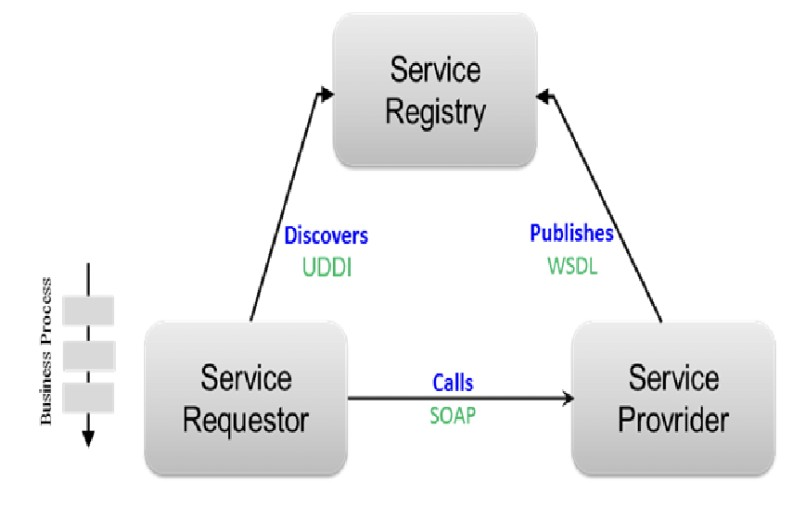
\includegraphics[width=0.8\textwidth]{chapter-2/tiga-elemen-service.jpg}
  \caption{Tiga Elemen pada Interaksi Service, \parencite{abugessaisa2023}}
  \label{fig:tiga-elemen-service}
\end{figure}

\textit{Service requestor} mengirimkan permintaannya serta kebutuhannya kepada \textit{service registry} untuk dicarikan service yang sesuai dengan kebutuhannya. Namun pada beberapa kasus khusus, \textit{service requestor}
sudah memiliki \textquotedblleft contract \textquotedblright dengan \textit{provider} tujuannya sehingga bisa langsung melakukan \textit{request} ke \textit{provider} tanpa bantuan dari \textit{service registry}.

Service \textit{provider} menyediakan \textit{service} yang dapat dikonsumsi oleh publik, agar \textit{service} nya dapat digunakan oleh requestor, \textit{service} \textit{provider} akan memberikan list \textit{services} yang dimiliki kepada registry untuk disimpan pada sebuah \textquotedblleft catalogue \textquotedblright yang dimiliki oleh registry.\textit{Service registry} berperan sebagai penengah dalam komunikasi \textit{requestor} dan \textit{provider}. \textit{Service registry} memiliki \textquotedblleft catalogue \textquotedblright yang menyimpan list berbagai macam \textit{service provider} yang dapat digunakan oleh \textit{service requestor}.

Dengan adanya ketiga elemen tersebut, interaksi pada \textit{services} dapat berjalan sehingga menciptakan suatu fungsionalitas seperti proses bisnis ataupun pemenuhan kebutuhan lainnya.


\section{\textit{Service discovery}}

\textit{Service discovery} adalah proses mencari layanan yang tersedia dan relevan untuk permintaan tertentu berdasarkan deskripsi semantik fungsional dan non-fungsional. \parencite{klusch2014servicediscovery}. \textit{Servie discovery} merupakan masalah yang sangat penting untuk menyelesaikan masalah konfigurasi. \textit{Service discovery} memungkinkan perangkat dan layanan untuk saling menemukan satu sama lain, mengatur diri, dan berkomunikasi dengan lancar. Namun, seringkali \textit{service discovery} tidak dimanfaatkan secara baik sehingga menghabiskan waktu untuk mencari layanan secara aktif dan mengatur perangkat dan program secara manual. Terkadang, konfigurasi layanan memerlukan keahlian khusus lainnya yang tidak berhubungan dengan apa yang ingin dicapai, sehingga hal ini membuat proses menjadi terhambat. Service discovery membantu untuk mengatasi masalah ini dengan membuat proses ini lebih otomatis dan mudah dilakukan \parencite{ServiceDiscovery}.

Dalam pengaplikasiannya terdapat beberapa \textit{pattern} yang dapat diaplikasikan dalam implementasi \textit{service discovery}. Menurut \parencite{micoservicearchitecture}, terdapat lima \textit{pattern} yang dapat digunakan ketika mengimplementasikan \textit{service discovery} yaitu \textit{3rd Party Registration, Client Side Serivce, Self Registration, serta Server-side service discovery}. Masing masing \textit{pattern} memiliki keunggulan dan kegunaan khusus sehingga perlu dipahami fungsi dari setiap \textit{pattern}.

\subsection{\textit{3rd Party Registration}}
\textit{3rd Party Registration pattern} adalah solusi yang digunakan pada kasus ketika service dapat di-\textit{register} dan \textit{unregister} pada \textit{registar} atau \textit{provider} nya. Solusi ini mewajibkan untuk melakukan registrasi kepada \textit{registar} ketika layanan baru dinyalakan dan melakukan \textit{unregister} ketika layanan dimatikan. layanan \textit{3rd party} yang bertanggung jawab sebagai \textit{registar} untuk mengelola hal ini \parencite{3rdpartyintegration}. Beberapa \textit{tools} yang telah menyediakan sistem layanan seperti ini yaitu \textit{Netflix Prana} yang akan bertindak sebagai \textit{side car} untuk aplikasi non-\textit{JVM} seperti Eureka ataupun AWS \textit{autoscaling groups} yang akan secara otomatis untuk meregister dan menghilangkan EC2 instance pada \textit{load balancer} nya.

Keuntungan untuk menggunakan \textit{pattern} ini ialah proses pembuatan kode yang mudah karena bergantung kepada \textit{3rd party} untuk proses registrasinya. Serta layanan \textit{3rd party} pun akan bertanggung jawab untuk melakukan pengecekan secara berkala agar sistem terus aktif sehingga meningkatkan \textit{availabilty} sistem. Namun, terdapat beberapa kekurangan diantaranya layanan \textit{3rd party} ini hanya bisa untuk melakukan \textit{discovery} secara umum. Seringkali dibutuhkan suatu solusi spesifik yang menjawab permasalahan khusus yang tidak bisa hanya diselesaikan dengan solusi seperti ini, perlu dibuat solusi \textit{custom} yang dapat menambah komponen baru ataupun arsitektur lain yang dapat menyelesaikan masalah tersebut \parencite{3rdpartyintegration}.

\subsection{\textit{Client Side}}
\textit{Client Side pattern} adalah suatu solusi \textit{service discovery} dengan proses \textit{client} yang mencari lokasi \textit{service} yang ingin dituju. \textit{Client} akan mencari lokasi dari tujuan dengan cara melakukan \textit{query} ke \textit{service registry} sehingga lokasi dari \textit{service} yang dituju dapat ditemukan secara dinamis dan \textit{runtime}. Beberapa keunggulan dari \textit{pattern} ini adalah mengurangi kompleksitas dan latensi karena mengurangi jumlah \textit{node} yang perlu di kunjungi. Namun salah satu kekurangannya yaitu meningkatnya kompleksitas kode yang dibuat, karena proses pencarian \textit{service} diletakkan di \textit{client} maka proses pencarian dan perubahan sepenuhnya dibebankan pada \textit{client}. Hal ini membuat proses pencarian tidak \textit{scalable} dan sulit ketika akan melakukan perubahan \parencite{clientsidediscovery}. Visualisasi dari \textit{client side service discovery} dapat dilihat pada \textbf{Gambar \ref{fig:client-side-discovery}}

\begin{figure}[ht]
  \centering
  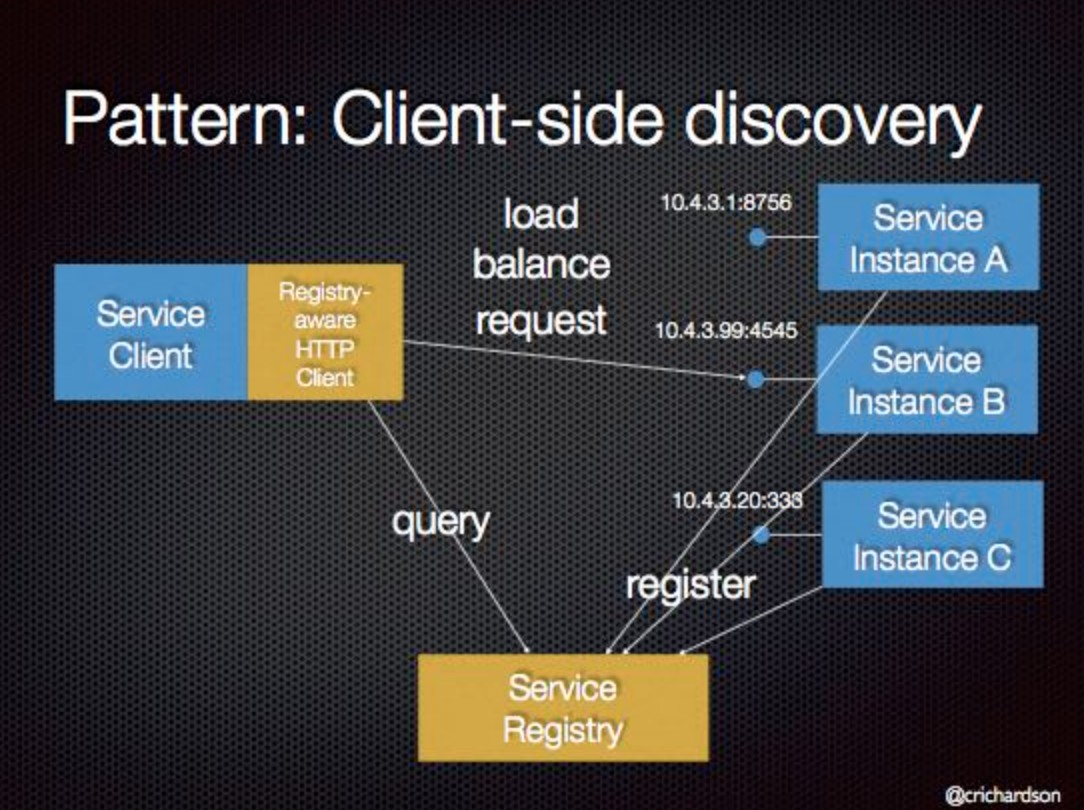
\includegraphics[width=1\textwidth]{resources/chapter-2/client-side-discovery.jpg}
  \caption{Visualisasi \textit{client side discovery} \parencite{clientsidediscovery} }
  \label{fig:client-side-discovery}
\end{figure}

\subsection{\textit{Self Registration}}
\textit{Pattern self registration service discovery} merupakan \textit{pattern} yang mudah untuk dilakukan. Pada dasarnya \textit{pattern} ini mirip dengan \textit{3rd party registration} yaitu sistem akan meregister \textit{service} ketika service dinyalakan dan \textit{service} akan di-\textit{unregister} ketika dimatikan. Meskipun solusi ini sederhana namun terdapat dua halangan diantaranya

\begin{enumerate}
  \item \textit{service} yang \textit{crash} harus dapat di-\textit{unregister} dari \textit{registry}
  \item \textit{service} yang sedang tidak bisa melayani permintaan harus di-\textit{unregister} dari \textit{registry} untuk menghindari terjadinya \textit{crash}
\end{enumerate}

Selain itu \textit{client} juga harus melakukan poling untuk mendapatkan data terbaru \textit{service} yang sedang aktif dan dapat menerima permintaan \parencite{selfregistration}.

\subsection{\textit{Server-side}}
Solusi ini memiliki visualisasi yang sama dengan \textit{client side discovery} pada \textbf{Gambar \ref{fig:client-side-discovery}}. Perbedaan yang mencolok yaitu alih alih \textit{client} yang melakukan request ke \textit{service registry}, \textit{client} akan melakukan \textit{request} kepada \textit{load balancer} dan \textit{load balancer} lah yang akan melakukan pencarian layanan mana yang sedang aktif dan dapat menerima permintaan. Cara ini merupakan cara yang paling umum digunakan untuk melakukan \textit{scaling} pada \textit{service} \parencite{servicesidediscovery}.


\section{Kubernetes}

Kubernetes adalah sebuah solusi \textit{open source} yang berguna untuk melakukan orkestrasi berbagai aplikasi yang telah dibungkus dalam suatu lingkungan yang disebut sebagai \textit{container}. Kubernetes berfungsi untuk melakukan \textit{deployment} otomatis, \textit{auto scaling} secara otomatis, serta membuat \textit{network} untuk menghubungkan \textit{container} dengan \textit{container} lainnya. Kubernetes membantu mengelola dan mempercepat proses pengembangan layanan yang rumit dengan skala yang besar \parencite{helmkubernetes}.

Kubernetes memiliki beberapa komponen yang digunakan ketika mengelola layanan. \textit{Node, pod, service} dan \textit{deployment} merupakan empat komponen utama yang sering kali menjadi komponen utama ketika membuat suatu layanan dengan Kubernetes. \textit{Node} dapat dianalogikan dengan lingkungan \textit{virtual machine} yang memiliki kemampuan terbatas. \textit{Pod} merupakan suatu tempat untuk menjalankan berbagai macam \textit{container} di dalamnya. Satu \textit{pod} dapat memiliki lebih dari satu \textit{container} untuk dioperasikan. \textit{Service} berfungsi untuk membuka akses eksternal ke dalam \textit{pod} yang secara umum bersifat internal dan tidak dapat diakses dari luar. Terakhir, yaitu \textit{deployment} adalah suatu konfigurasi untuk menjalankan layanan yang akan dibuat, konfigurasi \textit{deployment} juga melingkupi komponen \textit{pod} dan \textit{service}.

Kubernetes memiliki fitur seperti \textit{auto scaling, self-healing, device discovery, load balancing} serta \textit{rollout} dan \textit{rollback}. \textit{Auto scaling} sering digunakan untuk menjaga sistem untuk terus beroperasi dengan cara melakukan replikasi layanan dengan jumlah yang ditentukan. \textit{Self healing} memastikan bahwa layanan yang sedang mengalami kegagalan dapat diperbaiki secara otomatis. \textit{Rollout} dan \textit{Rollback} sering digunakan ketika melakukan proses \textit{deployment} untuk mencegah adanya \textit{downtime} ketika meluncurkan layanan versi baru. Seluruh fitur yang disebutkan bekerja sama untuk membuat kubernetes dapat mengelola aplikasi dalam skala yang masif dan mempertahankan kualitas layanan yang dibuat.

\subsection{\textit{Pod component}}

\textit{Pod} merupakan abstraksi unit atau komponen terkecil pada Kubernetes untuk memudahkan proses pengembangan. \textit{Pod} merupakan sebuah lingkunan linux yang digunakan secara bersama namun memiliki sumber daya yang terpisah dan terbatas melalui teknologi linux cgroups dan namespace untuk menjalankan satu atau lebih \textit{container}. \textit{Pod} bersifat \textit{ephemeral} sehingga seluruh sumber daya akan hilang apabila \textit{pod} mengalami kegagalan \parencite{pod}.

Untuk memastikan bahwa layanan dapat selalu berjalan dengan baik, semua kegiatan yang berkaitan dengan \textit{pod} mulai dari \textit{scaling} hingga \textit{health check} akan dilakukan oleh Kubernetes. Kubernetes akan bertanggung jawab untuk melakukan \textit{penjadwalan} serta pencocokan konfigurasi maupun siklus hidup dari \textit{pod} tersebut. Dengan abstraksi \textit{pod}, proses pengembangan layanan menggunakan Kubernetes semakin mudah untuk dipahami dan dilakukan.

\subsection{\textit{Service component}}

Service merupakan suatu abstraksi untuk membuat \textit{pod} dapat diakses secara eksternal. \textit{Pod} bersifat dan \textit{ephemeral} dan tidak dapat diakses dari luar \textit{pod}. Melalui abstraksi \textit{service} Kubernetes, \textit{pod} tersebut dapat diakses secara eksternal dengan cara membuat suatu layanan intermediet untuk meneruskan \textit{request} dari eksternal.
Layanan intermediet yang disediakan oleh \textit{service} diantaranya \textit{ClusterIp, NodePort, LoadBalancer} dan  \textit{ExternalName}.

ClusterIP bersifat internal dan sangat berkaitan erat dengan \textit{pod}. Apabila \textit{service} tidak dibuat konfigurasinya, \textit{pod} akan selalu memiliki \textit{service} dengan tipe \textit{ClusterIP}. \textit{NodePort} dan \textit{LoadBalancer} akan membuat \textit{pod} dapat ditemukan oleh layanan eksternal dan diakses melalui perangkat lain. Kedua tipe tersebut akan membuat sebuah \textit{endpoint} untuk meneruskan \textit{request} yang masuk berdasarkan label yang diletakan ketika membuat \textit{pod} \parencite{service}
\subsection{\textit{Deployment component}}

\textit{Deployment} merupakan abstraksi yang menggabungkan kedua abstraksi \textit{pod} dan \textit{service}. \textit{Deployment} dapat melihat kondisi seluruh sistem pada saat keadaan awal maupun keadaan berubah. \textit{Deployment} akan menyimpan keadaan sistem secara berkala pengecekan secara deklaratif untuk mendeteksi perubahan keadaan sistem saat ini dengan keadaan sistem yang diinginkan \parencite{deployment}.

\textit{Deployment} memiliki fitur \textit{rollout} dan \textit{rollback} untuk meningkatkan \textit{availability} layanan. \textit{rollback} berarti melakukan penurunan versi dari layanan yang saat ini sedang berjalan sedangkan \textit{rollout} untuk melakukan \textit{upgrade} layanan. Kedua fitur ini berjalan dengan cara membuat \textit{replica} dari layanan yang sedang berjalan untuk mencegah penurunan \textit{availability}. Ketika \textit{deployment} ingin menaikkan versi layanan yang digunakan, \textit{deployment} akan membuat \textit{pods} dengan versi terbaru. Ketika \textit{pods} ini sudah aktif beroprasi dan memiliki status \textit{healthy}, layanan dengan versi sebelumnya baru bisa dihapus \parencite{deployment}.

% Node merupakan suatu lingkungan terisolasi yang menjadi komponen dasar dalam pengelolaan aplikasi dengan kubernetes. 

\section{Kubernetes distribution}
Dalam penelitian ini akan dibahas tiga distribusi Kubernetes, yaitu KubeEdge, MicroK8s, serta K3s. Masing masing dari distribusi ini memiliki kegunaan dan fungsi nya masing masing. Walaupun semuanya memiliki \textit{support} untuk IoT namun setiap distribusi memiliki cara unik tersendiri untuk menyelesaikan masalahnya.

\subsection{KubeEdge}
KubeEdge merupakan solusi \textit{edge architecture} \textit{open source} yang mengembangkan Kubernetes secara lebih jauh untuk domain spesifik yaitu IoT \parencite{kubeedge}. Arsitektur KubeEdge memungkinkan untuk melakukan konfigurasi perangkat IoT yang berada di \textit{edge} secara terpusat melalui komponen \textit{cloud}. Dengan adanya dua komponen \textit{edge core} dan \textit{cloud core}, komunikasi antara platform aplikasi menjadi \textit{seamless}.

Untuk menghubungkan \textit{cloud core} dengan \textit{edge core}, KubeEdge menggunakan sebuah \textit{controller} yang dapat melakukan \textit{device discovery} terhadap \textit{edge core}. Setelah \textit{edge core} ditemukan, \textit{controller} akan meneruskan \textit{request} ke komponen berikutnya yaitu \textit{Sync Service}. KubeEdge menggunakan KubeBus untuk melakukan komunikasi antara \textit{cloud} dan \textit{edge}, KubeBus menggunakan protokol HTTP untuk meneruskan \textit{request} dari \textit{cloud core} menuju \textit{edge core}. Setelah \textit{request} diterima oleh \textit{edge core}, akan digunakan protokol MQTT untuk menerima ataupun mengirim data dari perangkat IoT ke \textit{edge core} dan juga sebaliknya. Ilustrasi arsitektur dapat dilihat pada gambar \ref*{fig:arsitektur-kube-edge}.

\begin{figure}[ht]
  \centering
  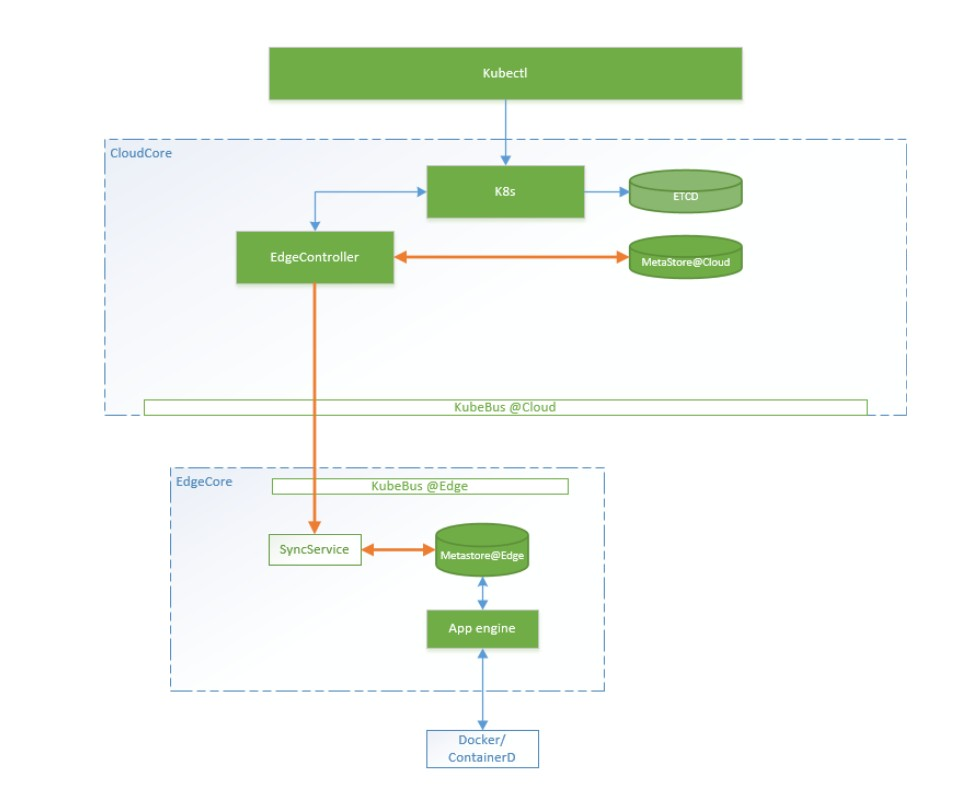
\includegraphics[width=0.5\textwidth]{resources/chapter-2/arsitektur-kube-edge.jpg}
  \caption{Arsitektur KubeEdge \parencite{kubeedge}}
  \label{fig:arsitektur-kube-edge}
\end{figure}

\subsection{Microk8s}
MicroK8s adalah sebuah platform \textit{open-source} yang digunakan untuk mengotomatisasi distribusi, \textit{scaling}, dan manajemen aplikasi yang berbasis kontainer. MicroK8s menyediakan fungsionalitas inti pada Kubernetes, dengan ukuran yang kecil, dan dapat di-\textit{scale} dari satu node hingga menjadi kluster produksi yang besar \parencite{microk8s}.

Dengan mengurangi penggunaan sumber daya yang dibutuhkan untuk menjalankan Kubernetes, MicroK8s memungkinkan penggunaan Kubernetes dalam berbagai lingkungan, seperti:

\begin{enumerate}
  \item Mengubah Kubernetes menjadi alat pengembangan yang ringan.
  \item Menjadikan Kubernetes tersedia untuk digunakan dalam lingkungan minimal seperti GitHub CI (Continuous Integration).
  \item Menyesuaikan Kubernetes untuk aplikasi IoT pada perangkat dengan sumber daya terbatas.
\end{enumerate}


\subsection{K3s}
K3s adalah sebuah platform \textit{open-source} yang memfasilitasi penggunaan Kubernetes dengan ukuran yang lebih ringan dan mudah diimplementasikan. K3s dikembangkan untuk memudahkan distribusi dan manajemen Kubernetes dalam lingkungan yang lebih sederhana dan bersifat minimalis. K3s dibuat untuk mendukung pengembangan pada ranah IoT karena K3s memiliki dukungan sepenuhnya untuk arsitektur ARM serta cocok untuk digunakan pada lingkungan \textit{edge} dan IoT \parencite{k3s}.

K3s memiliki dua komponen utama, yaitu \textit{server} dan \textit{agent}. \textit{Server} dapat dikatakan sebagai sebuah \textit{control plane} atau \textit{master node} yang digunakan pada K3s dan berfungsi untuk mengatur seluruh permintaan ataupun \textit{request} dari \textit{agent}. \textit{Server} memiliki tanggung jawab penuh terhadap masing masing \textit{agent} yang terhubung mulai dari menyimpan data dari masing masing \textit{agent}, \textit{controller}, serta \textit{scheduler} \parencite{k3s}. Di sisi lain, \textit{agent} berfungsi sebagai \textit{slave node} yang akan mengeksekusi semua perintah dari \textit{server} atau \textit{master node}. Ilustrasi arsitektur dapat dilihat pada gambar \ref{fig:arsitektur-k3s}.

\begin{figure}[ht]
  \centering
  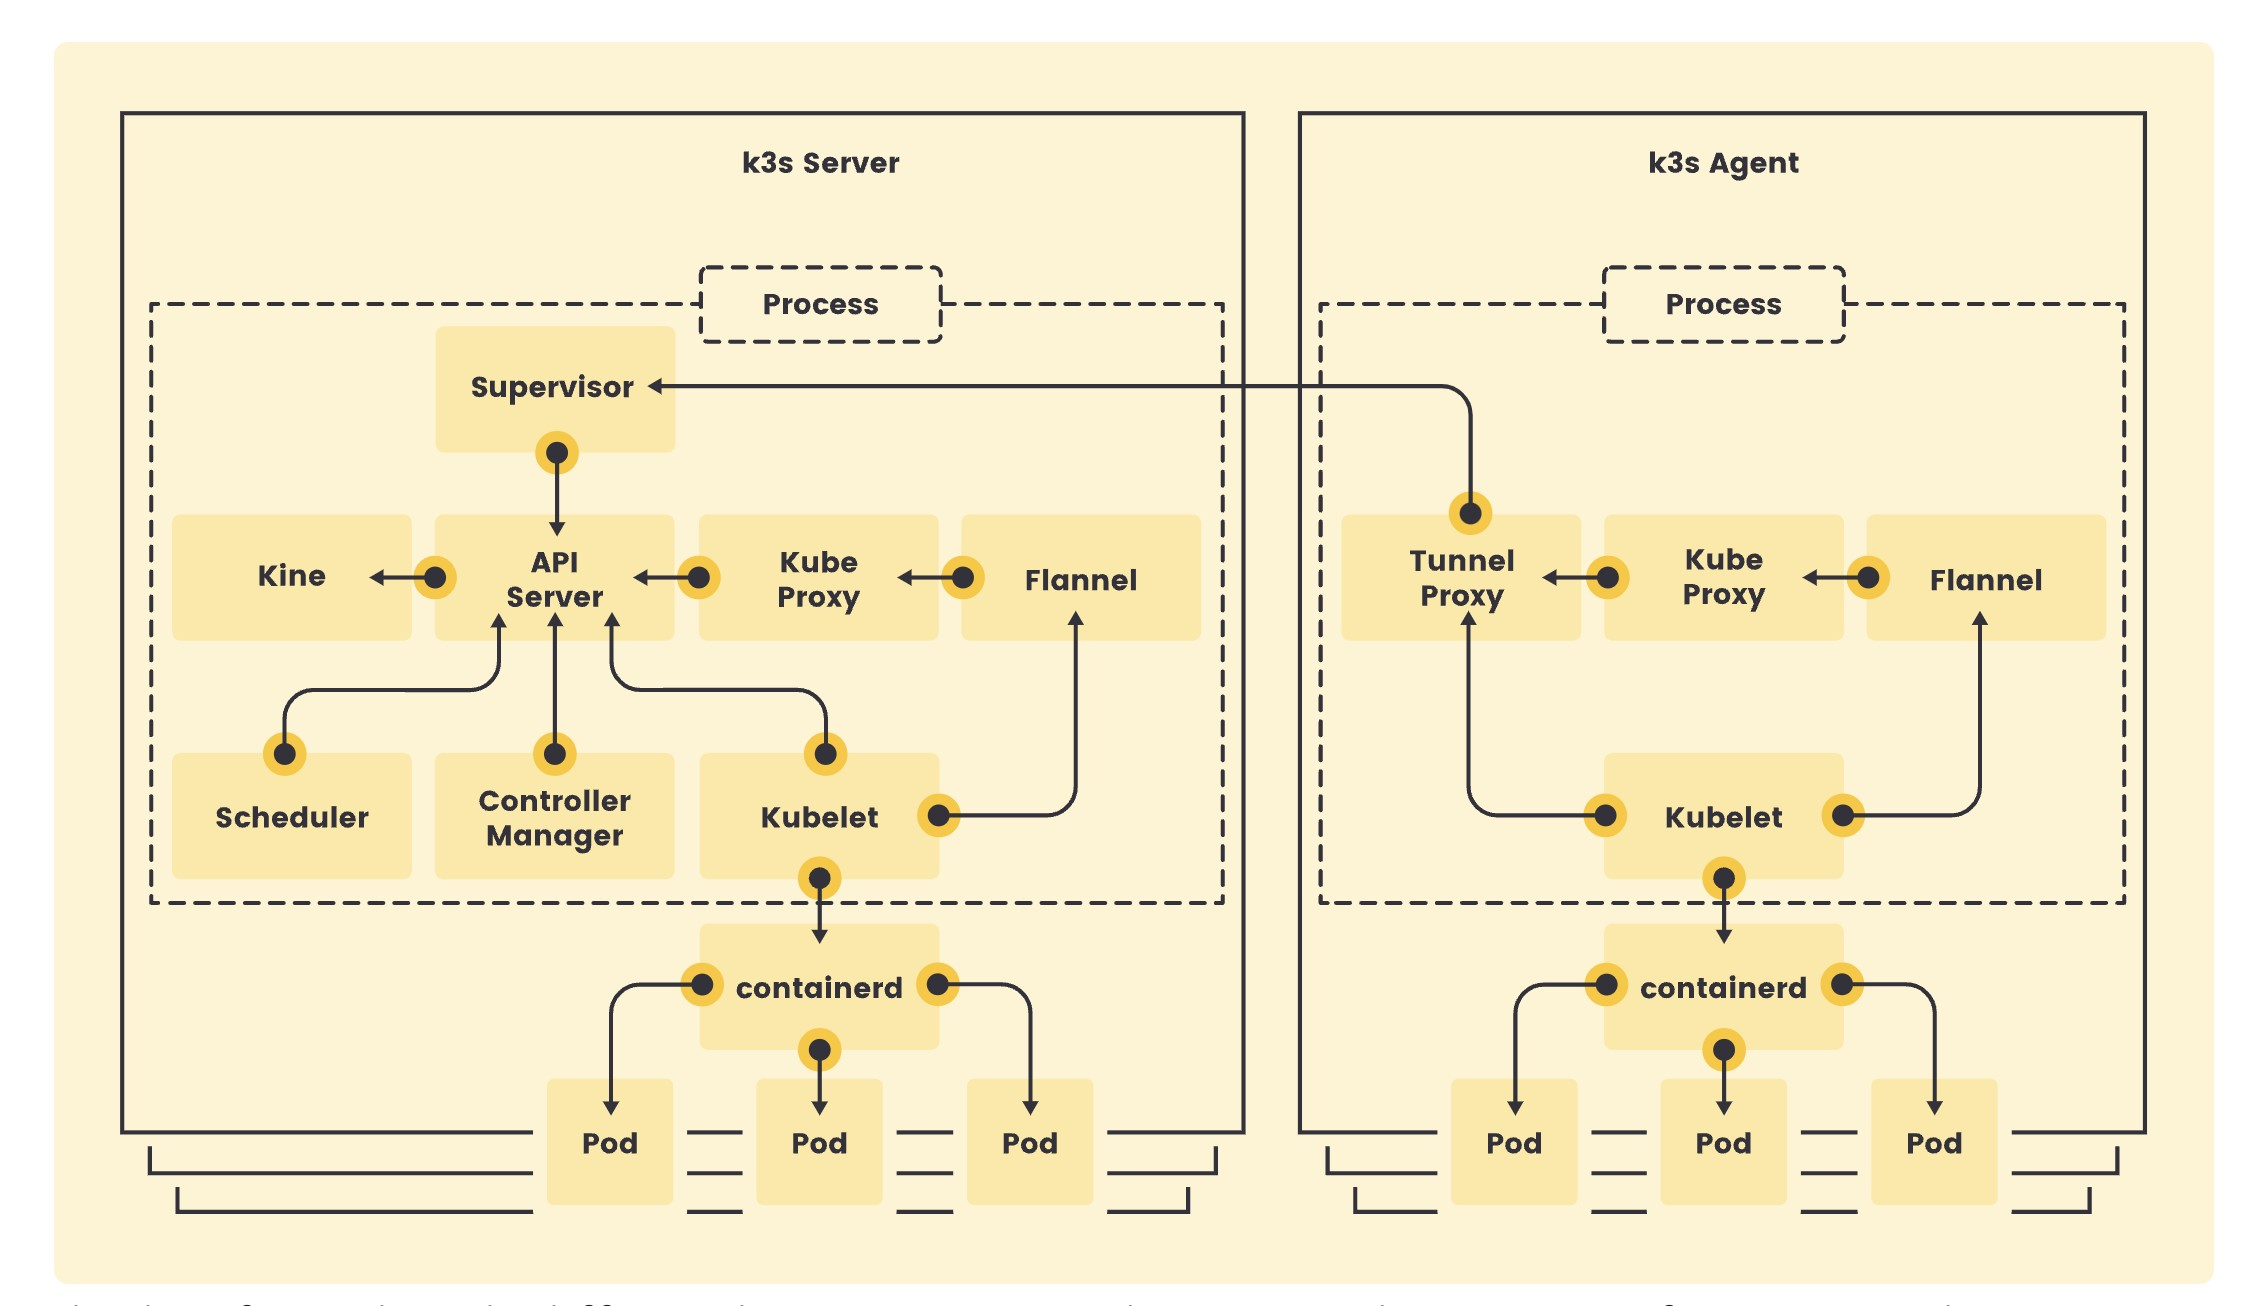
\includegraphics[width=1\textwidth]{resources/chapter-2/arsitektur-k3s.jpg}
  \caption{Arsitektur K3s \parencite{k3s}}
  \label{fig:arsitektur-k3s}
\end{figure}

\pagebreak

\section{\textit{IoT}}

\textit{Internet of Things (IoT)} adalah paradigma teknologi yang mengintegrasikan objek fisik dengan sensor, perangkat keras, dan teknologi jaringan, memungkinkan objek-objek ini untuk mengumpulkan dan bertukar data secara \textit{real-time}. Konsep ini merupakan perwujudan dari evolusi teknologi informasi, di mana objek sehari-hari bertransformasi menjadi entitas cerdas yang mampu berinteraksi dengan lingkungan sekitarnya dan jaringan digital secara lebih luas. \textit{IoT} memperkenalkan kemungkinan baru dalam otomatisasi dan pengambilan keputusan yang berbasis data, membuka jalan bagi inovasi lintas sektor \parencite{madakam2015internet}.

\begin{figure}[ht]
  \centering
  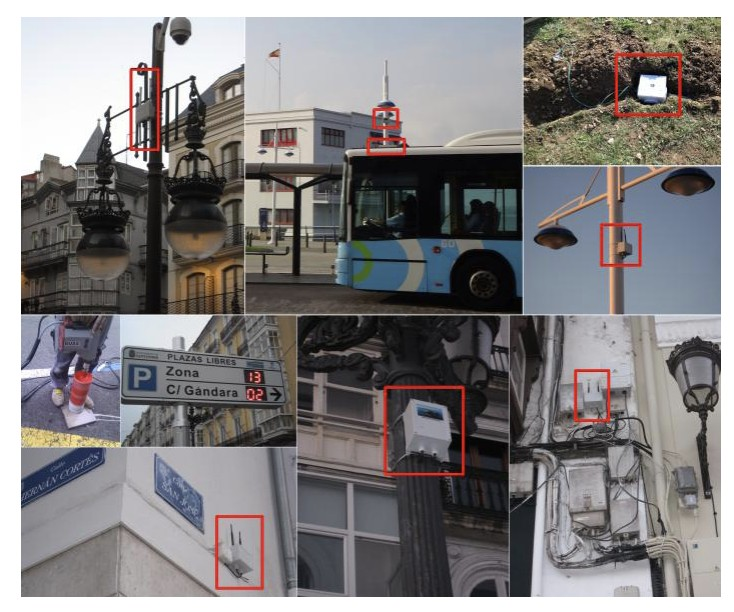
\includegraphics[width=0.8\textwidth]{resources/chapter-2/gambar-iot.jpg}
  \caption{Perangkat IoT yang Terdapat pada Lingkungan Sekitar \parencite{sotres2017practical}}
  \label{fig:iot-kehidupan-sehari-hari}
\end{figure}

\textit{IoT} memiliki aplikasi yang luas di berbagai sektor, termasuk industri, kesehatan, transportasi, dan pertanian. Dalam sektor industri, \textit{IoT} memungkinkan otomatisasi proses dan pemantauan efisiensi mesin secara real-time. Di bidang kesehatan, \textit{IoT} berkontribusi pada pengembangan perangkat medis yang terhubung untuk pemantauan kesehatan pasien. Dalam transportasi, \textit{IoT} mendukung pengembangan kendaraan otonom dan sistem manajemen lalu lintas cerdas. Di sektor pertanian, \textit{IoT} digunakan untuk memantau kondisi tanah dan iklim, membantu petani dalam pengambilan keputusan seperti pada gambar \ref{fig:iot-kehidupan-sehari-hari}

Dalam penerapannya \textit{IoT} dapat dibagi menjadi tiga lapisan, yaitu lapisan persepsi, lapisan jaringan, dan lapisan aplikasi secara berurutan. Lapisan persepsi bertanggung jawab atas pengumpulan data dalam \textit{IoT}. Lapisan ini terdiri dari berbagai jenis sensor, seperti sensor suhu, sensor kelembaban, RFID, kamera, GPS, dan sebagainya. Lapisan jaringan terdiri dari berbagai jenis jaringan, seperti internet, jaringan komunikasi 2G dan 3G, serta jaringan siaran. Lapisan jaringan terutama digunakan untuk mengumpulkan data dari lapisan persepsi dan memproses data tersebut untuk lapisan aplikasi. Terakhir yaitu Lapisan aplikasi, Lapisan ini adalah antarmuka antara pengguna dan \textit{IoT}. Banyak aplikasi, termasuk logistik, rantai pasokan, pertanian, industri, keamanan publik, pengelolaan perkotaan, telemedis, rumah pintar, transportasi pintar, dan pemantauan lingkungan, diaktifkan melalui \textit{IoT} \parencite{SmartHomeSystemBasedOnIoTTechnologies}.

Seiring bertambahnya jumlah perangkat \textit{IoT} perlu dibuat suatu cara agar sistem \textit{scalable}. \textit{Device discovery} merupakan salah satu masalah yang perlu diatasi untuk membuat sistem \textit{IoT} yang \textit{scalable} karena dapat meningkatkan \textit{quality of service} sehingga meningkatkan availabilty \parencite{DeviceDiscovery}. Tidak hanya itu, banyak munculnya perangkat \textit{IoT} baru yang memerlukan \textit{update} secara berkala menimbulkan masalah baru yaitu sulitnya untuk melakukan \textit{update} untuk setiap perangkat yang ada apabila jumlahnya semakin meningkat sehingga peran \textit{remote deployment} menjadi sangat penting dalam menyelesaikan masalah ini \parencite{RemoteDeployment}.

\section{Penelitian dan Riset Terkait}
\label{sec:riset-terkait}
Berikut adalah beberapa penelitian dan riset yang pernah dilakukan sebelumnya dan berhubungan dengan tugas akhir ini.

\subsection{LEONORE, \textit{Large-Scale Provisioning of
    Resource Constrained
    IoT Deployments}}
Riset dilakukan oleh Michael Vogler, Johannes M. Schleicher, Christian Inzinger, Stefan Nastic, Sanjin Sehic and Schahram Dustdar dari Vienna University of Technology. Riset ini menjelaskan mengenai cara pembuatan sebuah infrastruktur untuk melakukan \textit{provisioning} perangkat \textit{IoT} dalam skala besar.

\subsection{China Electronic Toll Colleciton}
China memiliki masyarakat yang sangat banyak dan setiap masyarakat memiliki sekurang kurangnya satu kendaraan. Seiring bertambah nya masyarakat di China, maka jalanan yang ada di China akan semakin penuh dengan kendaraan yang akan menghasilkan kemacetan terutama pada tol bagian pembayaran. Untuk mengatasi masalah ini China menggunakan \textit{Electronic Toll Colleciton (ETC)} yang di integrasikan dengan setiap kendaraan untuk mempercepat proses ini \parencite{penelitianterkait1}.

China menggunakan KubeEdge untuk melakukan proses \textit{deployment} \textit{ETC} untuk 100,000 \textit{nodes} dengan total 500,000 aplikasi yang diluncurkan menggunakan KubeEdge tersebar untuk 29 dari 34 provinsi. Proses \textit{deployment} dilakukan secara otomatis dengan membuat sistem \textit{workflow engine} pada kubernetes sehingga proses \textit{deployment} dapat dilakukan dengan cepat dan mudah. Dengan menggunakan metode ini sistem pembayaran tol di China menjadi 10x lebih cepat dari sebelumnya \parencite{penelitianterkait1}.

\begin{figure}[ht]
  \centering
  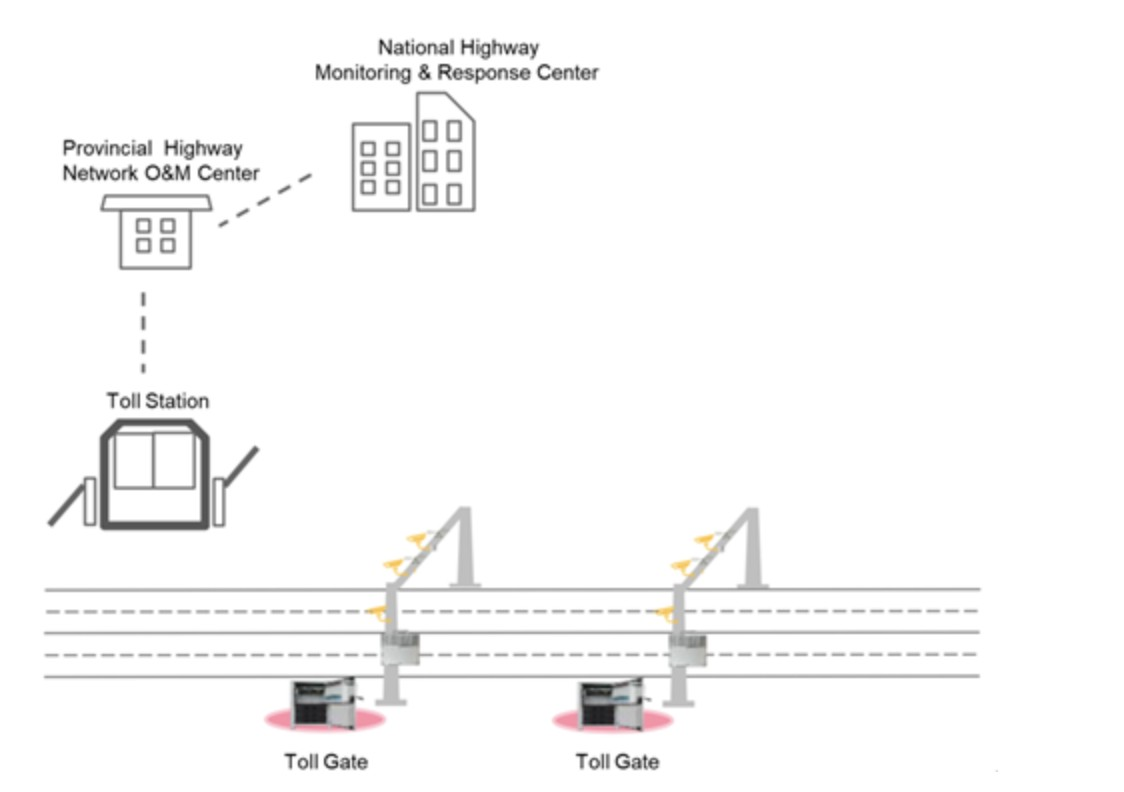
\includegraphics[width=0.8\textwidth]{resources/chapter-2/china-highways.jpg}
  \caption{Implementasi Sistem \textit{ETC} di China \parencite{penelitianterkait1}}
  \label{fig:china-highways}
\end{figure}

\begin{figure}[ht]
  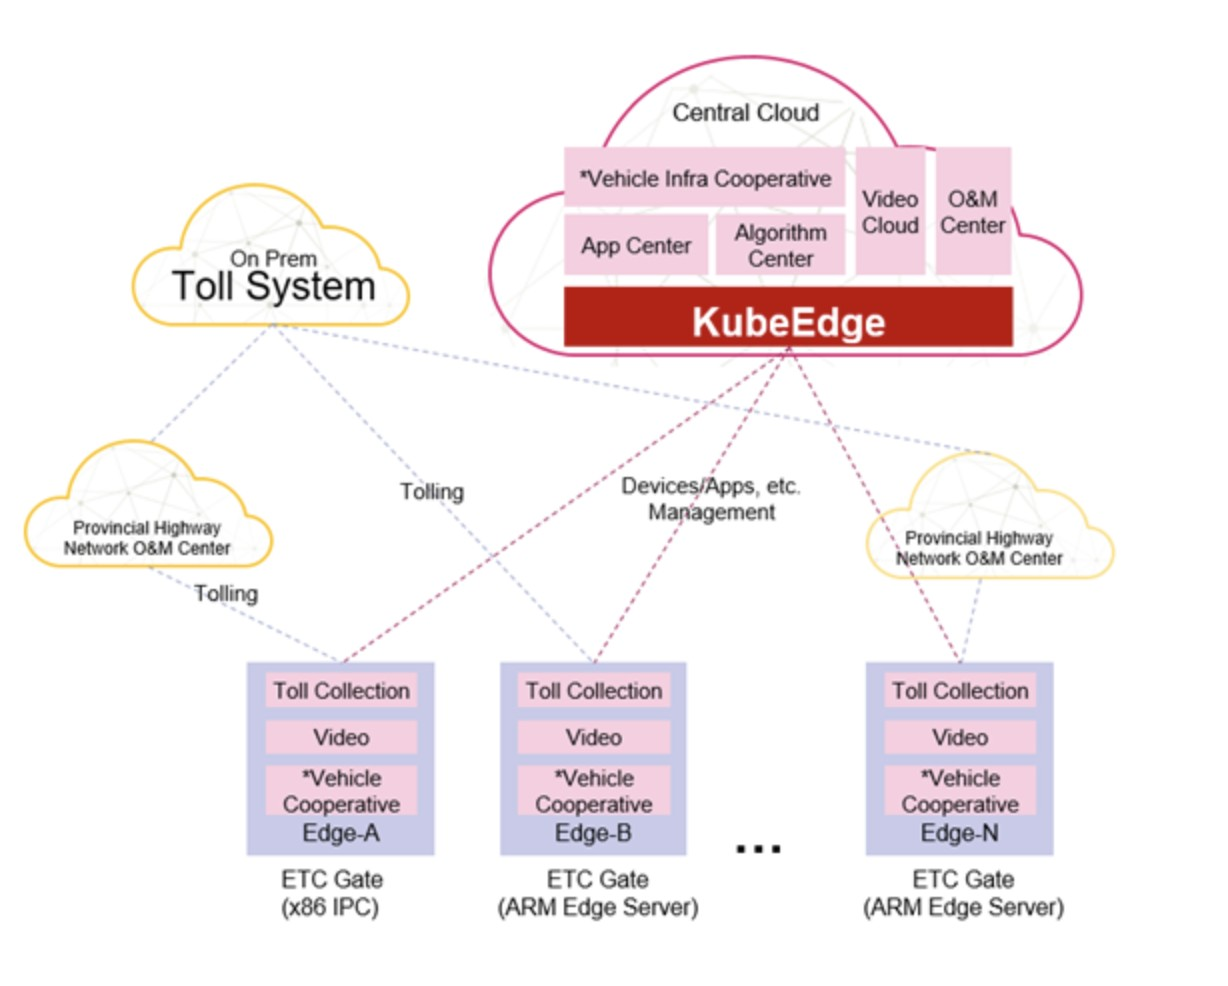
\includegraphics[width=0.8\textwidth]{resources/chapter-2/arsitektur-china-highways.jpg}
  \caption{Arsitektur Sistem \textit{ETC} di China \parencite{penelitianterkait1}}
  \label{fig:architecture-china-highways}
\end{figure}
\subsection{A Model for the Remote Deployment, Update, and Safe Recovery for Commercial Sensor-Based IoT Systems}
Penelitian ini menggali tantangan-tantangan khusus terkait infrastruktur yang didedikasikan untuk penyebaran dan manajemen aplikasi secara jarak jauh. Penelitian ini membahas tantangan-tantangan manajemen terkait sistem sensor IoT dan mengusulkan sebuah cara serta metodologi untuk mengatasi hal tersebut.

Penelitian ini mengimplementasikan solusi sebagai sistem infrastruktur perangkat lunak untuk produk IoT bisnis yang lengkap. Penelitian ini melakukan \textit{deployment} pada 100 perangkat penjual minuman yang tersebar di tiga lokasi. Setiap perangkat bergantung pada sensor yang memantau statusnya dan pada \textit{gateway} yang mengendalikan perilakunya. Arsitektur sistem dapat dilihat pada gambar \ref{fig:architecture-remote-deployments}.

\begin{figure}[ht]
  \centering
  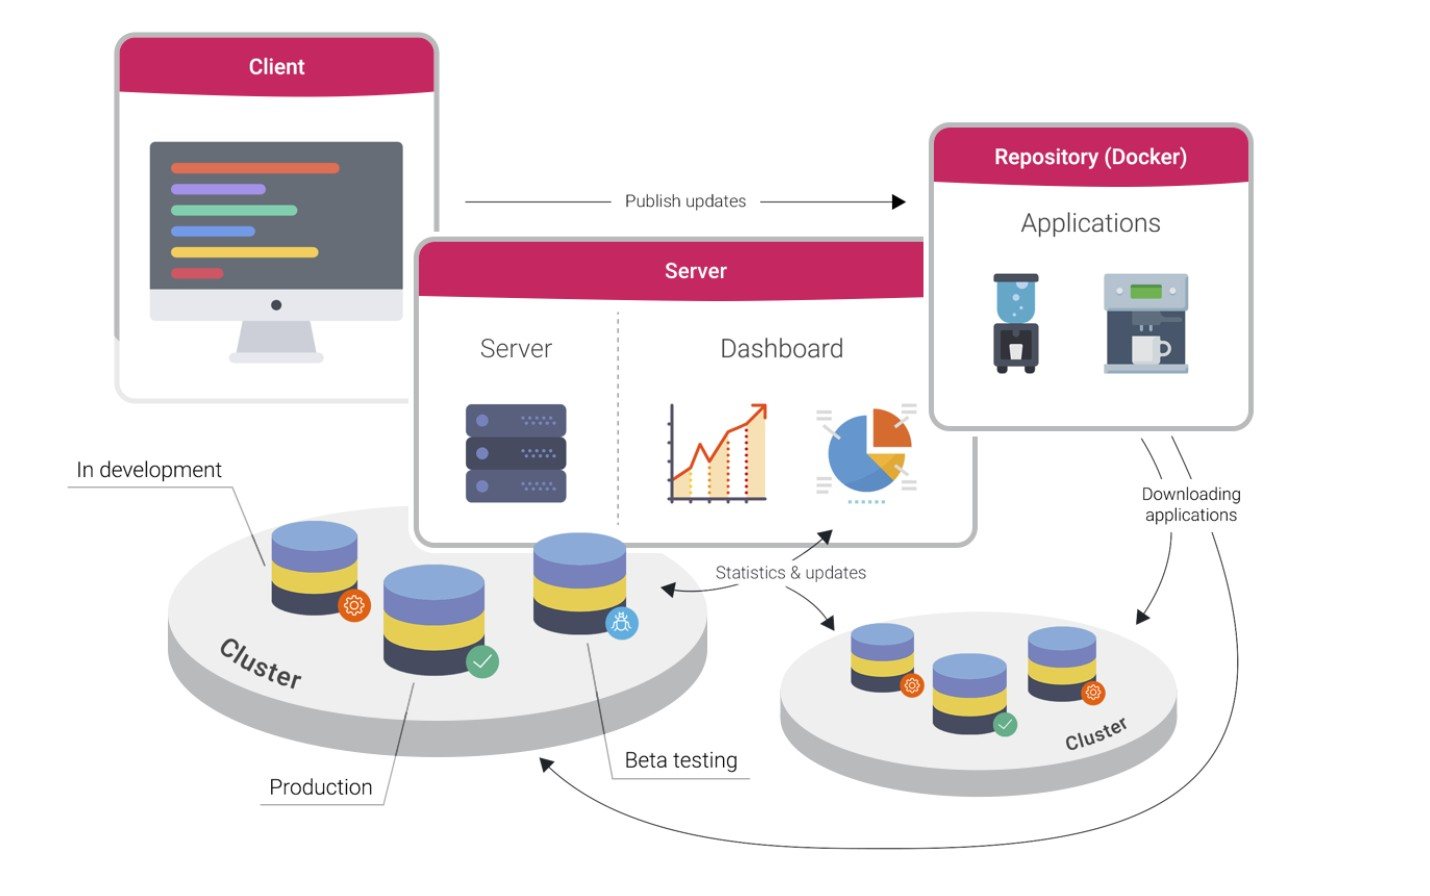
\includegraphics[width=0.8\textwidth]{resources/chapter-2/arsitektur-remote-deployment.jpg}
  \caption{Arsitektur Remote \textit{Deployment} \parencite{RemoteDeployment}}
  \label{fig:architecture-remote-deployments}
\end{figure}

Selama penelitian ini berlangsung, penelitian ini berhasil menerima 133 \textit{update} pada perangkat IoT. 80\% perangkat beroperasi tanpa gangguan selama 250 hari. Sedangkan, 20\% mengalami kegagalan akibat faktor eksternal. Dari 80\% tersebut, 30\% mengalami kegagalan pembaruan sementara akibat kapabilitas perangkat yang berkurang \parencite{RemoteDeployment}.

Solusi yang dibuat penelitian ini mengandalkan keamanan serta \textit{failsafe} yang dapat melakukan \textit{remote deployment} dengan baik serta aman sehingga dapat mendeteksi kegagalan yang terjadi pada perangkat dan melakukan \textit{recovery} dengan cepat. Berikut merupakan beberapa cara untuk melakukan \textit{remote deployment} atau seringkali disebut sebagai OTA \textit{(Over the air)}.

\begin{figure}[ht]
  \centering
  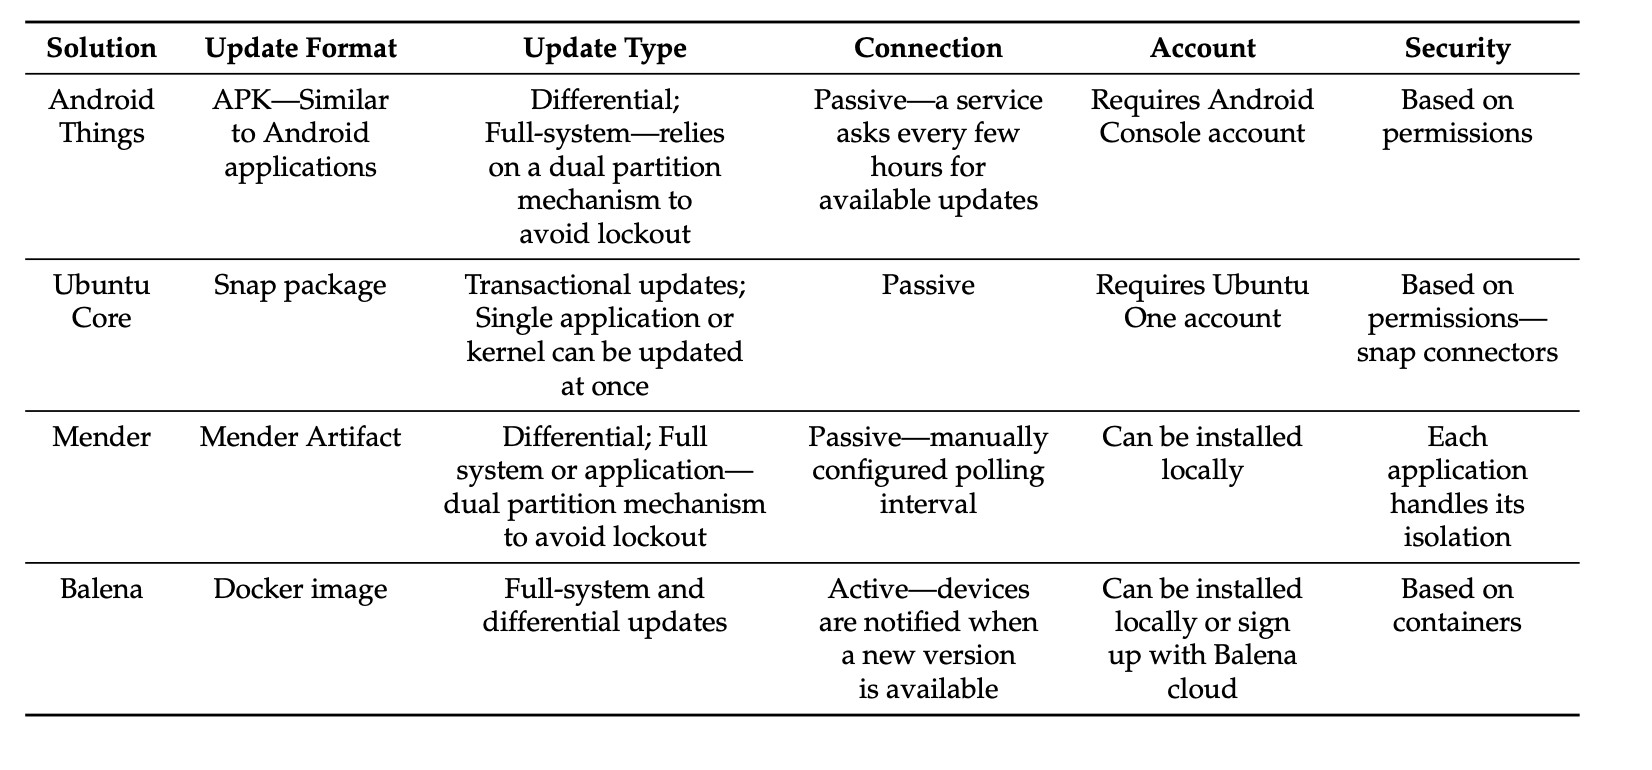
\includegraphics[width=0.8\textwidth]{resources/chapter-2/perbandingan-remote-deployment.jpg}
  \caption{Perbandingan Tata Cara \textit{Remote Deployment} \parencite{RemoteDeployment}}
  \label{fig:comparison-remote-deployments}
\end{figure}

Dapat dilihat dari gambar \ref{fig:comparison-remote-deployments} bahwa terdapat berbagai solusi untuk berbagai tipe \textit{remote deployment}. Pada kasus ini, dapat dibuat suatu cara yang mengadopsi \textit{update type} serta koneksi dari keempat tipe tersebut. Perangkat melakukan \textit{polling} kepada \textit{server} untuk mengecek apakah terdapat versi terbaru atau tidak. Selain itu, dari sisi \textit{Server} juga dapat membuat suatu notifikasi yang dapat diterima oleh perangkat jika terdapat \textit{update} baru yang siap digunakan.
% \section{Penelitian dan Riset Terkait}
Berikut adalah beberapa penelitian dan riset yang pernah dilakukan sebelumnya dan berhubungan dengan tugas akhir ini.

\subsection{\textit{Deep Learning-Based Autoscaling Using Bidirectional Long Short-Term Memory for Kubernetes}}
Riset dilakukan oleh Nhat Minh, Dang Quang dan Myungsik Yoo dari \textit{Department of Information Communication Convergence Technology, Soongsil University}, Seoul, Korea Selatan yang dipublikasikan 23 April 2021. Secara umum, penelitian tersebut membahas pengembangan \textit{autoscaling} menggunakan \textit{deep learning} dengan \textit{Bidirectional Long Short-Term Memory} (Bi-LSTM) untuk melakukan \textit{autoscale} untuk \textit{web server} dengan memperhatikan metrik penggunaan prosesor dan memori.

Menurut riset ini, \textit{Autoscaling} merujuk pada proses yang secara dinamis mengalokasikan sumber daya, dan dapat dikelompokkan menjadi dua jenis: reaktif dan proaktif. Pendekatan proaktif menganalisa data historis, melakukan prediksi, dan menentukan keputusan \textit{scaling}. Sedangkan, pendekatan reaktif melakukan keputusan \textit{scaling} berdasarkan kondisi saat itu dengan sekumpulan \textit{threshold}. Solusi dengan pendekatan reaktif sangat mudah diimplementasikan namun memilih nilai yang tepat untuk menjadi ambang batas menjadi sulit karena beban kerja yang terus-menerus berfluktuasi tergantung pada perilaku pengguna, \parencite{riset1}.

Perbandingan terhadap model ARIMA dan LSTM juga dilakukan pada riset ini. Secara keseluruhan, hasil eksperimen dengan beberapa data set seperti \textit{The FIFA World Cup} dan \textit{NASA} yang berisikan logs web dari instansi terkait. Ditemukan bahwa error ketiga model ini (Bi-LSTM, ARIMA, dan LSTM) tidak signifikan. Meskipun begitu, Bi-LSTM memiliki kecepatan yang signifikan dan akurasi yang sedikit lebih baik dibanding kedua model lainnya. Namun, tentu saja ini bergantung pada konfigurasi model Bi-LSTM serta algoritma pada fase analisa. Sedangkan untuk uji kompleksitas, ARIMA sangat unggul karena sederhana dan tidak memerlukan banyak percobaan terhadap konfigurasi serta algoritma.

Kakas yang dipakai untuk melakukan eksperimen dan pengembangan pada riset tersebut adalah \textit{Tensorflow}, \textit{Keras} dan \textit{Statsmodels} yang berguna untuk membangun model ARIMA, LSTM, dan Bi-LSTM. Sedangkan untuk teknologi yang dipakai adalah \textit{JMeter}, \textit{HAProxy}, \textit{Prometheus}, \textit{Docker} dan \textit{Kubernetes}.

Dijelaskan riset ini memakai arsitektur sistem bernama \textit{Monitor-Analyse-Planning-Execution} (MAPE) loop. Untuk lebih jelasnya, bisa dilihat pada gambar \ref{fig:mape}. Secara singkat, pada fase monitor, sistem akan mengambil data melalui \textit{application metric collector} lalu dilanjutkan dengan fase analisis yaitu memanfaatkan Bi-LSTM untuk mengolah data yang sudah didapat sebelumnya. Kemudian, fase perencanaan adalah fase melakukan prediksi dan kalkulasi terhadap \textit{scaling} yang akan dilakukan. Dan akan diakhiri oleh fase eksekusi apabila diperlukan adanya perubahan alokasi dari fase perencanaan. Fase tersebut akan diulang secara terus menerus.

\begin{figure}[h]
    \centering
    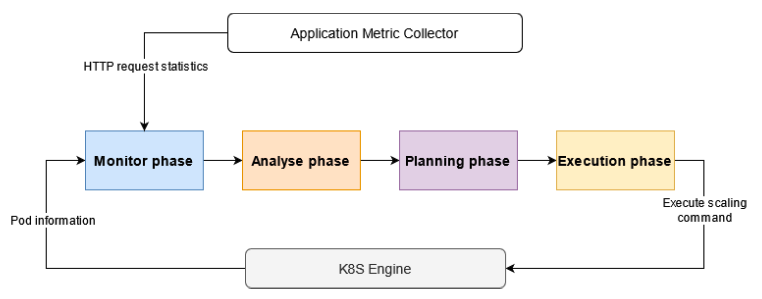
\includegraphics[width=0.8\textwidth]{chapter-2/mape.png}
    \caption{Arsitektur Sistem MAPE, \parencite{riset1}}
    \label{fig:mape}
\end{figure}

\subsection{Penelitian Lainnya}

Adapun \textit{autoscaler} yang sudah dikembangkan dan dibahas di banyak penelitian lain. Pendekatan dan metode yang digunakan sangat variatif. Gambaran umum mengenai penelitian lain yang berhubungan dengan \textit{autoscaler} menggunakan model prediksi, \textit{threshold} atau \textit{rule based} maupun \textit{machine learning} bisa dilihat pada tabel \ref{tab:overview-autoscaler}.

\begin{longtable}{|p{2in}|c|p{1in}|c|p{0.8in}|}

    \caption{Tabel Penelitian Lain terkait Pengembangan Metode \textit{Autoscaling}} \label{tab:overview-autoscaler} \\

    \hline
    \rowcolor{gray!30}\multicolumn{1}{|c|}{\textbf{Paper}} & \textbf{Virtualisasi} & \multicolumn{1}{|c|}{\textbf{Metrik}} & \textbf{Pendekatan} & \multicolumn{1}{|c|}{\textbf{Metode}} \\
    \hline
    \endfirsthead
    %
    \endhead
    %
    \textit{Intelligent Workload Factoring for a Hybrid Cloud Computing Model}, \parencite{zhang} & VM & \textit{Request Rate} & Reaktif & ARIMA \tabularnewline

    \textit{Autonomic Vertical Elasticity of Docker Containers with Elasticdocker}, \parencite{al2017autonomic} & \textit{Container} & Prosesor, Memori & Reaktif & \textit{Rule-based} \tabularnewline

    \textit{Horizontal Pod Autoscaler}, \parencite{hpa2} & \textit{Container} & Prosesor & Reaktif & \textit{Rule-based} \tabularnewline

    \textit{A Novel Resource Prediction and Provisioning Scheme in Cloud Data Center}, \parencite{rpps} & \textit{Container} & Prosesor & Proaktif & ARMA \tabularnewline

    \textit{Workload Prediction Using ARIMA Model and Its Impact on Cloud Applications QoS}, \parencite{workloadprediction} & VM & \textit{Request Rate} & Proaktif & ARIMA \tabularnewline

    \textit{Resource Elasticity Controller for Docker-based Web Applications}, \parencite{resourceelasticity} & \textit{Container} & \textit{Request Rate} & Proaktif & ARIMA \tabularnewline

    \textit{Combining Time Series Prediction Models using Genetic Algorithm to Autoscaling Web Applications Hosted in the Cloud Infrastructure}, \parencite{tspwithga} & - & \textit{Request Rate} & Proaktif & \textit{Genetic Algorithm} \tabularnewline

    \textit{Predicting Cloud Resource Provisioning using Machine Learning Techniques}, \parencite{predictcloudrsrc} & - & \textit{Task Length} & Proaktif & \textit{Artificial Neural Network} \tabularnewline

    \textit{Auto-scaling Microservices on IaaS under SLA with Cost-Effective Framework}, \parencite{asmicrocosteff} & VM & \textit{Request Rate} & Proaktif & \textit{Artificial Neural Network}, \textit{Recurrent Neural Network} \tabularnewline

    \textit{Machine Learning-based Auto-scaling for Containerized Applications}, \parencite{mlbasconapps} & \textit{Container} & \textit{Request Rate} & Proaktif & LSTM \tabularnewline

    \textit{Adaptive Horizontal Scaling of Microservices using Bi-LSTM}, \parencite{adaptivehsmicro} & \textit{Container} & Prosesor, Memori & Gabungan & Bi-LSTM \tabularnewline

    \hline
\end{longtable}



% \section{\textit{Inverted Index}}
\label{sec:invertedindex}

\textit{Inverted Index} merupakan struktur data yang biasa digunakan untuk mesin pencari \parencite{invertedindex2}. Tujuan dari implementasi struktur data ini pada mesin pencari adalah untuk mengoptimalkan kecepatan query dalam mencari dokumen yang mengandung kata kunci tertentu. Struktur data ini melakukan pemetaan terhadap kata dan kumpulan tupel yang berisikan \textit{identifier} (ID) dokumen dan posisi karakter \parencite{invertedindex}. Struktur data ini biasanya dipakai untuk menggantikan \textit{Forward Index}. \textit{Forward Index} adalah struktur data yang menyimpan seluruh kata dalam sebuah dokumen sehingga jika \textit{forward index} di-\textit{query}, maka akan memerlukan iterasi sekuensial pada setiap dokumen dan kata kunci untuk membuktikan dokumen relevan. Sumber daya waktu, memori, dan pemrosesan yang dibutuhkan untuk melakukan query semacam itu tidak realistis dan praktis karena nyatanya, mesin pencari harus melakukan hal tersebut ke ratusan hinga jutaan dokumen. Dengan inverted index yang dibuat, query dapat diselesaikan dengan cara langsung melompat ke \textit{identifier} (ID) kata kunci melalui \textit{random access} pada inverted index untuk mendapatkan \textit{identifier} (ID) dokumen dan posisi karakter.

% \section{\textit{Elastic Search}}
% \textit{Elastic Search} adalah aplikasi mesin pencarian RESTful.  \textit{Elastic Search} diciptakan sebagai pembungkus dan inovasi dari Apache Lucene yang sekedar hanya \textit{library} karena aplikasi yang beredar saat ini tidak hanya dibuat di atas Java dan membutuhkan fleksibilitas yang tinggi, sedangkan, Apache Lucene terkenal sangat sulit untuk orang awam yang tidak memahami istilah-istilah dan \textit{information retrieval}. \textit{Elastic Search} sendiri dibuat menggunakan Java namun menggunakan \textit{Application Programming Interface} RESTful melalui protokol HTTP sehingga aplikasi dengan bahasa apapun dapat dengan mudah menggunakan aplikasi ini. Tidak hanya itu, API dari \textit{Elastic Search} ini juga sudah sangat dipermudah sehingga pemakai tidak perlu mengetahui istilah-istilah dalam Apache Lucene. Sehingga, \textit{Elastic Search} ini sangat dekat dengan proses umum pada data seperti menyimpan, membaharui, menghapus, pengindeksan, pencarian, dan sebagainya.

\textit{Elastic Search} merupakan sebuah perangkat lunak \textit{open-source} yang ditulis menggunakan bahasa pemrograman Java. \textit{Elastic Search} dibangun di atas Apache Lucene. \textit{Elastic Search} menyimpan data secara terpusat untuk pencarian secepat kilat dan relevan \parencite{elasticsearchorigin}. Selain Apache Lucene, \textit{Elastic Search} memanfaatkan teknologi-teknologi lain untuk meningkatkan fungsionalitas dan kinerja, seperti Apache Hadoop untuk big data processing, Apache Spark untuk data analytics, dan Apache Storm untuk real-time stream processing.

\textit{Elastic Search} didesain sebagai sebuah sistem terdistribusi, yang berarti data yang disimpan pada \textit{Elastic Search} akan didistribusikan ke beberapa \textit{node} atau lebih dikenal sebagai \textit{sharding}, sehingga memungkinkan untuk meningkatkan kinerja, skalabilitas, dan ketahanan pada sistem. Sistem terdistribusi pada \textit{Elastic Search} dapat diatur dan dikonfigurasi agar dapat dijalankan pada beberapa \textit{node} yang terpisah atau pada \textit{cluster} yang terhubung, yang memungkinkan pengguna untuk menyimpan data yang sangat besar dan menjalankan query secara paralel pada beberapa node pada waktu yang bersamaan.

\textit{Elastic Search} dibuat untuk memudahkan pengguna mengakses data dan melakukan pencarian pada data yang besar dan kompleks dengan cepat dan efisien. Meskipun Apache Lucene telah menyediakan fitur-fitur yang bagus untuk \textit{indexing} dan \textit{searching}, tetapi Apache Lucene lebih fokus pada teknologi inti dan pengembangan secara \textit{information retrieval} seperti mengoptimisasi dan pengembangan \textit{indexing} dan \textit{searching}. Hal tersebut menyebabkan penggunaan Lucene memerlukan banyak pengaturan dan konfigurasi tambahan untuk bisa diintegrasikan dengan aplikasi yang lebih besar. Dalam hal ini, \textit{Elastic Search} hadir sebagai sebuah solusi yang lebih terintegrasi, mudah digunakan, dan dapat diatur secara fleksibel. \textit{Elastic Search} memanfaatkan Lucene sebagai mesin pencari, tetapi menambahkan banyak fitur-fitur dan fungsionalitas tambahan untuk meningkatkan kinerja dan kemudahan penggunaan. Selain itu, \textit{Elastic Search} dirancang sebagai aplikasi dengan sistem terdistribusi dan \textit{scalable} yang memungkinkan data terdistribusi di beberapa node atau \textit{sharding}, sehingga memungkinkan \textit{Elastic Search} untuk mengatasi masalah data yang sangat besar dan kompleks secara efektif dan efisien. Sedangkan, Lucene hanya pada batas kakas atau \textit{library}.

\textit{Elastic Search} dapat digunakan dengan protokol HTTP dan REST API. Dalam penggunaan dengan protokol HTTP, \textit{Elastic Search} menyediakan endpoint API RESTful HTTP yang dapat diakses oleh pengguna dengan memakai klien HTTP, seperti perintah cURL, \textit{Postman} atau \textit{web browser}. Pengguna dapat membuat permintaan HTTP seperti GET, POST, PUT, DELETE ke API endpoint melalui klien HTTP, dan \textit{Elastic Search} akan memberikan respon sesuai dengan permintaan.

Dalam \textit{Elastic Search} terdapat beberapa operasi yang dapat dilakukan, diantaranya:
\begin{enumerate}
    \item \textbf{\textit{Index}}
    
    Operasi ini akan dijelaskan secara khusus pada bagian selanjutnya, \ref{sec:index}.

    \item \textbf{\textit{Get}}
    
    Operasi \textit{Get} digunakan untuk mengambil dokumen individual berdasarkan ID-nya dari indeks tertentu.
    
    \item \textbf{\textit{Query}}
    
    \textit{Query} digunakan untuk melakukan pencarian dan pengambilan data yang sesuai dengan kriteria tertentu. \textit{Elasticsearch} menyediakan berbagai jenis query seperti pencarian teks lengkap, pencocokan kata kunci, pencocokan frasa, pencarian fuzzy, dan lain-lain.
    
    \item \textbf{\textit{Fetch}}
    
    \textit{Fetch} adalah proses pengambilan dokumen lengkap dari indeks setelah melakukan query. Saat ditemukan, \textit{Elasticsearch} mengambil dokumen dari indeks dan akan digunakan sebagai respon kepada pengguna.
    
    \item \textbf{\textit{Scroll}}
    
    \textit{Scroll} adalah mekanisme pengambilan dokumen yang banyak dari hasil pencarian tanpa perlu mengirimkan \textit{query} ulang. Hal ini menyebabkan pengambilan dokumen dapat menjadi lebih efisien dalam beberapa permintaan, namun, dalam beberapa kasus, bisa menjadi lebih lama untuk mengambil semua dokumen yang relevan.
    
    \item \textbf{\textit{Suggest}}
    
    \textit{Suggest} adalah mekanisme untuk memberikan saran atau \textit{autocompletion} saat pengguna memasukkan kata kunci atau frasa. Biasanya digunakan untuk \textit{autocompletion}, pengoreksi kesalahan pengejaan, dan saran pencarian lainnya.
    
    \item \textbf{\textit{Bulk}}
    
    \textit{Bulk} adalah operasi yang digunakan untuk memasukkan atau memperbarui beberapa dokumen dalam satu permintaan.
    
    \item \textbf{\textit{Flush}}
    
    \textit{Flush} adalah operasi yang digunakan untuk mengosongkan memori \textit{cache} dan menulis data yang tertunda ke disk. Operasi ini memastikan bahwa data yang ditulis telah disimpan secara permanen di indeks.
    
    \item \textbf{\textit{Refresh}}
    
    \textit{Refresh} adalah operasi yang digunakan untuk membuat perubahan yang terjadi pada indeks secara terlihat dan dapat dicari. Saat melakukan operasi indeks seperti menambahkan atau menghapus dokumen, perubahan tersebut tidak langsung terlihat oleh pencarian hingga dilakukan operasi refresh.
\end{enumerate}

% \section{Java \textit{Virtual Machine}}
\textit{Java Virtual Machine} atau JVM adalah program yang dapat membaca program java yang telah dikompilasi atau biasa dikenal sebagai \textit{java bytecode} dan menginterpretasikannya menjadi bahasa mesin yang dapat dieksekusi oleh komputer \parencite{java12}. Secara tidak langsung, JVM merupakan komponen utama dalam menjalankan program bahasa Java. Struktur JVM terdiri dari \textit{runtime data structure} di memori dan dua subsistem yang berhubungan langsung dengan \textit{runtime data structure} yaitu \textit{class loader} dan \textit{execution engine}. Semua program yang dibuat dengan Java akan dikompilasi ke \textit{java bytecode} yang nantinya akan diinterpretasikan oleh JVM untuk dieksekusi komputer.

\textit{Elastic Search}, yang terbuat dari bahasa Java, berjalan di atas platform Java Virtual Machine (JVM). JVM sendiri akan bertanggung jawab untuk menjalankan kode Java dan mengelola sumber daya yang dibutuhkan oleh program, seperti memori, prosesor, dan jaringan. Sehingga, JVM memiliki peran penting dalam menjalankan \textit{Elastic Search} dan memastikan kinerjanya baik. JVM menyediakan opsi pengaturan yang membuat pengguna dapat mengontrol alokasi memori dan penggunaan CPU pada aplikasi \textit{Elastic Search}. Dengan mengatur parameter JVM yang tepat, pengguna dapat memperbaiki kinerja \textit{Elastic Search} dan memaksimalkan penggunaan sumber daya sistem.

Parameter yang berhubungan erat dengan alokasi sumber daya pada \textit{Elastic Search} dan mempengaruhi kinerja JVM adalah parameter \textit{heap size} (-Xms dan -Xmx) yang mengatur ukuran \textit{heap memory} yang dialokasikan untuk JVM. \textit{Heap memory} adalah tempat JVM menyimpan objek dan data dari aplikasi Java yang sedang berjalan. Parameter -Xms menentukan ukuran \textit{heap memory} awal yang dialokasikan ketika JVM dimulai, sedangkan parameter -Xmx menentukan batas maksimal ukuran \textit{heap memory} yang dapat dipakai oleh JVM. Selain itu, terdapat parameter lain yang dapat mempengaruhi kinerja JVM dan \textit{Elastic Search}, seperti \textit{thread pool size}, \textit{circuit breaker settings}, dan lain-lain. Parameter-parameter ini dapat diatur melalui file konfigurasi \textit{Elastic Search} atau melalui command line arguments saat menjalankan \textit{Elastic Search}.

% \section{\textit{Indexing}}
\label{sec:index}

\textit{Indexing} adalah suatu teknik untuk menyusun kata-kata dan mengurangi usaha untuk mencari hal yang berkaitan dengan kata tersebut jika diperlukan, \parencite{database}. Secara umum, indeks banyak digunakan pada buku teks, basis data, dan sistem information retrieval. Seperti salah satu contoh tekniknya adalah \textit{Inverted Index} yang telah dijelaskan pada \ref{sec:invertedindex}.

Terdapat kelebihan penggunaan indeks, diantaranya:
\begin{enumerate}
    \item \textit{Indexing} dapat mempercepat proses pencarian data dengan membuat indeks dan mencocokkan kata kunci dengan indeks tersebut, sehingga mesin dapat menemukan data dengan lebih cepat.
    \item \textit{Indexing} dapat meningkatkan akurasi pencarian dengan menampilkan hasil pencarian yang lebih relevan dengan kata kunci yang dimasukkan.
\end{enumerate}

Namun, ada juga kelemahan dari penggunaan indeks, yaitu sebagai berikut.
\begin{enumerate}
    \item \textit{Indexing} memerlukan ruang penyimpanan tambahan untuk membuat indeks.
    \item Proses pembuatan \textit{indexing} memerlukan waktu, terutama jika data yang akan di-indeks sangat banyak.
\end{enumerate}

Sehingga, dapat disimpulkan penggunaan indeks sangat bermanfaat namun menambahkan biaya.
Pada kasus-kasus dokumen besar, penggunaan indeks pengaruhnya sangat besar karena mesin akan mencari data pada indeks terlebih dahulu sebelum mencari data pada dokumen asli. Hal ini dapat membantu mengurangi waktu pencarian dan menghemat penggunaan memori karena mesin tidak perlu membaca seluruh dokumen untuk menemukan data yang dicari. Namun, apabila \textit{indexing} dilakukan secara berlebihan, akan terdapat banyak indeks yang tidak terpakai dan hanya akan menambah kebutuhan memori.

% Konsep \textit{caching} sendiri adalah menyimpan data yang sering diakses pada level cache atau memori yang lebih dekat dengan CPU agar dapat diakses dengan cepat saat ingin melakukan pencarian, lihat gambar \ref{fig:cache-level}. \textit{Cache} sendiri biasanya memiliki ruang yang terbatas sehingga biasanya membuang data yang sudah tidak diakses sehingga jika dibutuhkan harus dicari ke \textit{storage}. Konsep ini ditiru oleh basis data dan aplikasi \textit{information retrieval} untuk mempercepat proses pencarian dengan memanfaatkan \textit{indexing} untuk mencari (lihat gambar \ref{fig:cache-app}) dan \textit{caching} untuk mengembalikan data yang sering diakses dengan memanfaatkan memori.

% \begin{figure}[h]
%     \centering
%     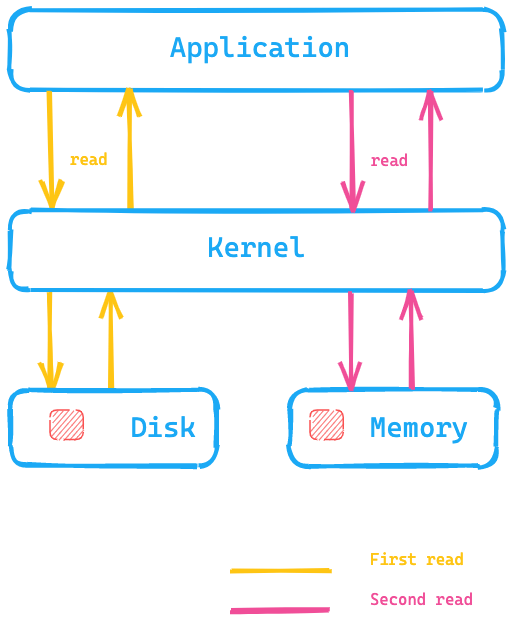
\includegraphics[width=0.5\textwidth]{chapter-2/cache-app.png}
%     \caption{Prinsip Cache pada Aplikasi}
%     \label{fig:cache-app}
% \end{figure}

% \begin{figure}[h]
%     \centering
%     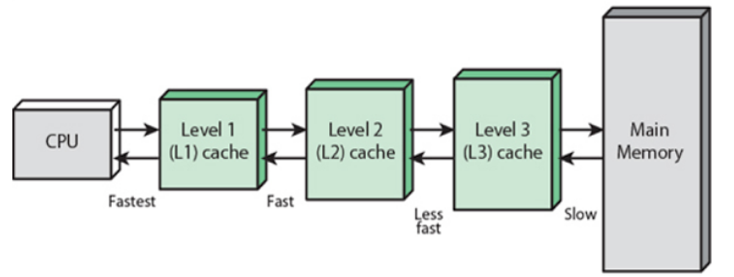
\includegraphics[width=0.5\textwidth]{chapter-2/cache-memory.jpeg}
%     \caption{Level-level pada Cache}
%     \label{fig:cache-level}
% \end{figure}

% \section{\textit{Caching}}
\textit{Caching} adalah teknik menyimpan data atau informasi yang sering digunakan secara lokal pada suatu tempat agar dapat diakses lebih cepat kedepannya. \textit{Caching} dapat digunakan untuk menyimpan hasil pencarian yang sering dilakukan oleh pengguna, sehingga jika pengguna melakukan pencarian yang sama, hasilnya dapat diambil dari \textit{cache} yang tersimpan dan tidak perlu melakukan pencarian.

Terdapat relevansi \textit{caching} dengan indeks, \textit{caching} dapat membantu meningkatkan kinerja sistem indeks dengan menyimpan hasil pencarian yang sering dilakukan dan mengaksesnya dari \textit{cache} saat pengguna melakukan pencarian yang sama. Dengan demikian, waktu dan sumber daya yang diperlukan untuk memproses pencarian dapat dihemat. Pengguna juga dapat mengakses hasil pencarian dengan lebih cepat karena data yang dicari sudah disimpan di \textit{cache} dan tidak perlu memproses ulang dari indeks. Namun, perlu diingat bahwa ukuran cache harus dibatasi, sehingga \textit{caching} tidak menggunakan memori secara berlebihan.

% \input{chapters/chapter-2/15-simulasi}
% \section{Pembelajaran Mesin}
% Pembelajaran Mesin adalah sebuah bidang pembelajaran yang mempelajari pemahaman dan membangun metode untuk "belajar" dengan memanfaatkan data untuk meningkatkan banyak aspek terutama efisiensi dan kualitas terhadap suatu rangkaian tugas. Algoritma pembelajaran mesin membangun model berdasarkan data sampel yang biasa disebut \textit{training data} untuk menghasilkan model yang dapat memprediksi atau membuat keputusan tanpa diprogram secara eksplisit, \parencite{ml}.

% \subsection{\textit{Reinforcement Learning}}
% \textit{Reinforcement learning} atau RL adalah bidang pembelajaran mesin yang mengotomasi sebuah agen untuk mengambil tindakan dan memaksimalkan \textit{reward} dari aksi yang dilakukan, \parencite{reinforcementlearning}. RL adalah salah satu paradigma dari tiga pembelajaran mesin dasar seperti \textit{Supervised Learning} dan \textit{Unsupervised Learning}. Singkatnya, RL membuat agen dapat mengoreksi pengetahuannya secara terus menerus agar dapat memaksimalkan fungsinya. Berbeda dengan \textit{Supervised Learning}, RL tidak memerlukan label dan tidak memerlukan secara eksplisit dikoreksi. Fokus dalam membangun RL, adalah mencari keseimbangan eksplorasi terhadap lingkungan baru dan eksploitasi terhadap pengetahuan yang dimiliki.

% penelitian terkait
% \blankpage
\chapter{Analisis Persoalan dan Rancangan Solusi}

Tujuan utama penulisan bab ini adalah untuk menguraikan rencana penyelesaian masalah tugas akhir sebelum dieksekusi. Bagian ini akan memaparkan proses analisis masalah hingga menjadi solusi.

\subsection{Analisis Permasalahan}
\label{sec:analisis-permasalahan}

Pada lingkungan \textit{IoT}, berbagai perangkat terhubung memainkan peran penting dalam mengumpulkan dan memproses data dari lingkungan sekitarnya. Perangkat ini sering kali terbatas sumber daya, memiliki kapasitas pemrosesan, memori, dan penyimpanan yang minim. Meskipun begitu, ada kebutuhan yang meningkat untuk mengerahkan logika aplikasi yang kompleks secara langsung ke perangkat-perangkat ini untuk meningkatkan efisiensi, mengurangi latensi, dan mendukung operasi \textit{offline} atau semi-\textit{offline}. Masalah utama yang muncul adalah bagaimana secara efisien mengelola dan mengerahkan komponen aplikasi pada skala besar dalam lingkungan yang sangat heterogen dan terbatas sumber daya.

Berdasarkan latar belakang yang telah diuraikan pada \textbf{Bagian \ref{sec:latar-belakang}}, masalah ini dapat diselesaikan dengan menggunakan \textit{remote deployment}. Namun, proses pembuatan layanan agar dapat melakukan \textit{remote deplotment} untuk perangkat yang heterogen menjadi hal yang cukup sulit, perlu dibuat sebuah sistem yang mengatur seluruh proses agar menjadi konsisten dan \textit{well documented}. Sistem ini juga bermanfaat untuk pengguna yang ingin mencoba mengembangkan sistem untuk menambah berbagai fitur kedepannya. Standar ini akan terdiri dari model \textit{deployment} serta layanan orkestrasi untuk membantu proses pengelolaan. Layanan orkestrasi, berperan cukup penting dalam sistem, dengan adanya layanan ini proses pengelolaan perangkat yang heterogen menjadi cukup mudah untuk dilakukan. Selain layanan orkestrasi, \textit{deployment plan} model pun perlu memiliki standar agar dapat digunakan oleh \textit{client} atau \textit{developer}.

Sistem dibuat dengan menyediakan infrastruktur yang berorientasi layanan untuk pengerahan komponen aplikasi yang elastis pada perangkat yang memiliki sumber daya yang terbatas pada IoT dengan skala besar. Sistem harus memiliki dukungan untuk melakukan \textit{deployment} berbasis push, serta mengetahui kondisi dari setiap perangkat. Sistem yang dibuat perlu memiliki cara untuk membuat sebuah resep deployment yang terdiri dari beberapa komponen iot serta
pemrosesan paket aplikasi yang disesuaikan dengan platform perangkat, dan mekanisme skalabilitas untuk mengelola penyebaran ke jumlah perangkat yang besar dengan efisien.

Untuk membuat implementasi dari sistem \textit{remote deployment}, terdapat beberapa rintangan yang perlu diatasi. Rintangan tersebut, dapat dirumuskan ke dalam poin-poin sebagai berikut.

\begin{enumerate}
  \item Kondisi saat ini belum banyak sistem \textit{IoT} yang dibuat dan diorkestrasi menggunakan \textit{kubernetes}
  \item Belum ada \textit{deployment plan} yang dapat mendefinisikan proses \textit{deployment} serta agar \textit{remote deployment} dapat diorkestrasi  dengan menggunakan \textit{kubernetes}
  \item Sistem dapat berjalan meskipun dalam kondisi buruk.
  \item Sistem dapat mengetahui kondisi dari masing masing perangkat serta proses \textit{deployment} yang sedang berjalan.
  \item Sistem dapat melakukan deployment dengan metode \textit{push}, sehingga setiap perangkat yang terhubung akan melakukan proses pembaruan secara otomatis.
\end{enumerate}


\section{Analisis Solusi}

Berdasarkan analisis permasalahan pada \ref{sec:analisis-permasalahan} serta studi literatur, Terdapat tiga alternatif solusi untuk mengatasi permasalahan tesrebut.
Mengembangkan sebuah sistem yang memiliki \textit{reliability} dan \textit{observability} yang baik dengan skalabilitas yang tinggi dengan menggunakan kubernetes dengan \textit{service mesh}. Membuat sistem dengan \textit{reliability} yang baik  menggunakan protokol \textit{MQTT}, serta peningkatan layanan internet pada setiap lingkungan disekitar perangkat \textit{IoT}.

\subsection{Perangkat IoT dibekali dengan Internet yang baik}
Salah satu cara untuk mengatasi masalah ini yaitu dengan menaruh internet yang baik disekitar perangkat \textit{IoT}. Dengan adanya hal ini, proses \textit{reliability} akan tercapai serta sistem juga akan memiliki latensi yang rendah. Namun, cara ini tidak optimal dan membutuhkan biaya yang cukup mahal.

Perlu ditempatkan internet yang baik di sekitar perangkat \textit{IoT} memerlukan biaya yang cukup banyak dan cara ini sepenuhnya bergantung pada kualitas \textit{internet service provider} yang digunakan. Apabila \textit{ISP} sedang mengalami penurunan kualitas dan membuat jaringan menjadi buruk maka cara ini sistem akan langsung \textit{unreliable}.

\subsection{Membuat sistem menggunakan protokol MQTT untuk melakukan pertukaran data}
Akan dibuat suatu sistem yang dapat berkomunkasi menggunakan protokol \textit{MQTT}. Sistem ini terdiri dua komponen, \textit{client} dan \textit{broker}. MQTT \textit{client} berfungsi untuk melkukan \textit{subscribe} ataupun \textit{publish} data ke MQTT \textit{broker}. MQTT \textit{broker} sendiri akan menyimpan data yang dikirim oleh sensor ataupun perangkat \textit{IoT} lainnya (publish) dan memiliki reliability yang sangat tinggi sehingga seberapa burukpun jaringannya akan tetap dapat diterima dengan baik \parencite{mqtt}.

\subsection{Membuat \textit{Smart Home System} berbasis Service Mesh dengan kubernetes}
Untuk membuat suatu sistem yang memenuhi dan menjawab permasalahan yang telah diangkat sebelumnya, dapat dibuat suatu sistem menggunakan kubernetes berbasis service mesh





% \subsection{Arsitektur standar untuk \textit{deployment} pada KubeEdge}
% Untuk membuat arsitektur pada KubeEdge perlu memerlukan beberapa konsiderasi terutama pada bagian \textit{EdgeCore}. Secara konsep arsitektur pada KubeEdge tidak jauh berbeda dari kubernetes pada umumnya, namun terdapat perbedaan cara berkomunkasi dari bagian \textit{cloud} dengan \textit{edge} serta komunikasi antar perangkat \textit{IoT} pada \textit{Edge} yang menggunakan MQTT. Dengan melakukan percobaan \textit{deploy} dengan KubeEdge dan melihat referensi pada \ref{sec:riset-terkait} proses standardiasi arsitektur akan mudah untuk dilakukan

% \subsection{Meningkatkan \textit{device discovery} pada layanan}
% Dengan melakukan integrasi dengan \textit{Service Mesh} proses \textit{device discovery} menjadi lebih mudah untuk dilakukan karena untuk setiap aplikasi yang di\textit{deploy} menggunakan KubeEdge, akan ditambah sebuah \textit{sidecar proxy} untuk proses penerimaan maupun pengiriman \textit{request}. Dengan adanya \textit{sidecar proxy} proses \textit{device discovery} menjadi lebih mudah untuk dilakukan.

% \subsection{Menurunkan \textit{low latency} pada layanan}
% Tantangan utama pada aplikasi yang terintegrasi dengan \textit{service mesh} adalah \textit{latency} akan dijamin bertambah karena adanya \textit{extra hop} yang digunakan saat pengiriman maupun penerimaan request. Untuk mengatasi masalah ini dapat digunakan metode lain untuk implementasi \textit{service mesh} seperti \textit{zero-trust tunnel} ataupun menggunakan \textit{eBPF}
% \subsection{Membuat sistem dengan skalabilitas yang baik}
% Dengan menggunakan kubernetes, khususnya \textit{KubeEdge} dapat dibuat sebuah konfigurasi file \textit{deployment} yang telah memenuhi semua \textit{requirements}. File ini akan menjadi acuan untuk proses \textit{deployment} kedepannya.

% \subsection{Membuat sistem dengan \textit{high availability} dan \textit{fault tolerant}}
% Dengan memanfaatkan keunggulan \textit{rollout} dan \textit{rollback} serta \textit{scaling} untuk \textit{deployment} pada kubernetes. Masalah ini menjadi mudah untuk diatasi karena secara umum kubernetes akan memastikan proses \textit{upgrade} ataupun \textit{downgrade} berjalan terlebih dahulu sebelum mematikan layanan yang lama. Karena pada \textit{IoT} memiliki \textit{spec} perangkat yang rendah, proses \textit{scaling} yang digunakan harus menjadi bagian yang dipertimbangkan

\section{Rancangan Solusi}
\label{sec:rancangan-solusi}

\subsection{Gambaran Umum}
Dengan segala kebutuhan yang sudah dianalisis, maka akan dibuat beberapa komponen penyusun sistem. Rencananya, sistem  akan dibuat menggunakan KubeEdge dan perangkat \textit{IoT} akan dibatasi jumlahnya sebanyak lima dan setiap perangkat akan diasumsikan sebagai \textit{cluster} yang berbeda.

\begin{figure}[h]
  \centering
  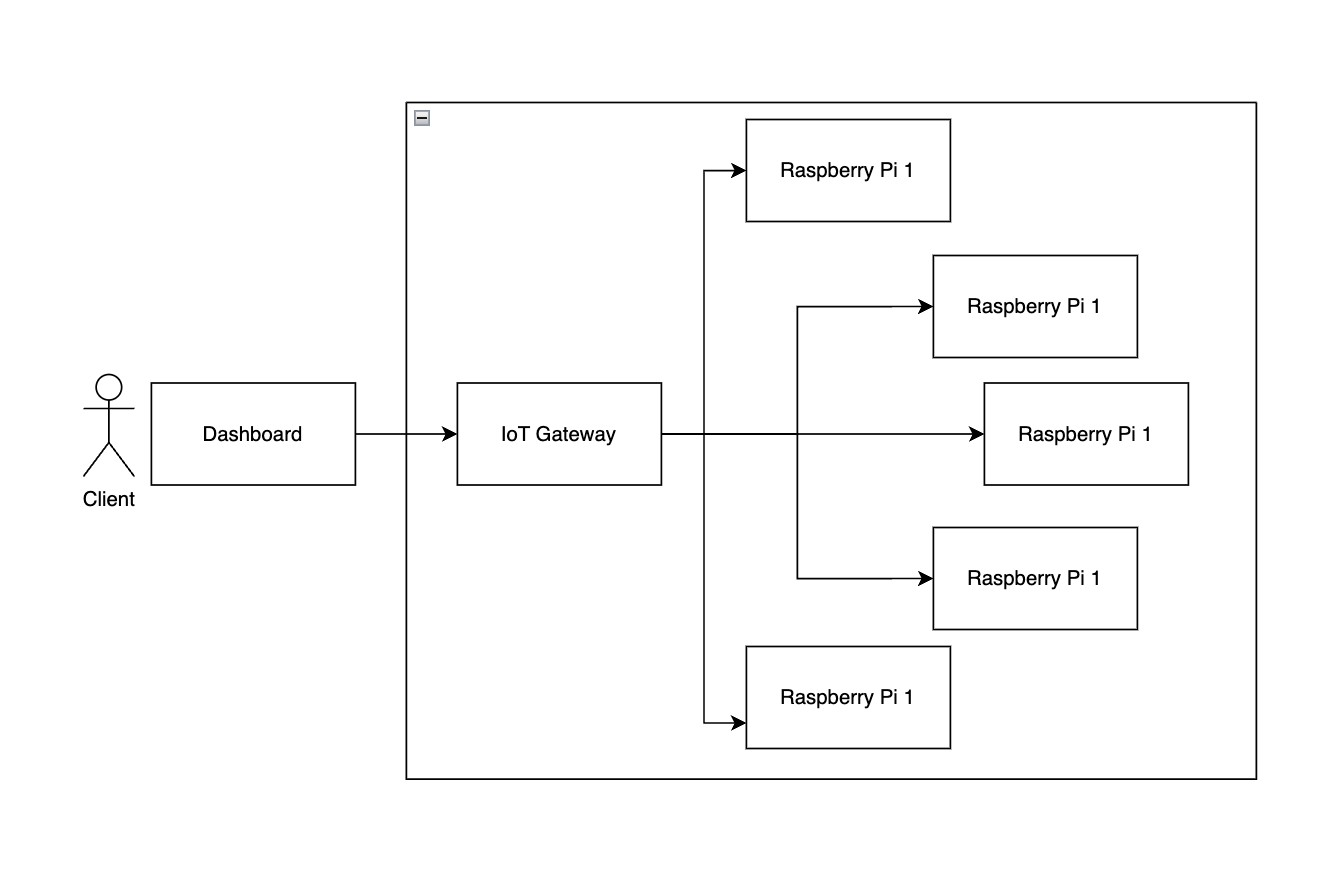
\includegraphics[width=0.5\textwidth]{resources/chapter-3/gambaran-umum-arsitektur.jpg}
  \caption{Gambaran umum arsitektur yang akan dibuat}
  \label{fig:gambaran-umum-arsitektur}
\end{figure}
% \chapter{Implementasi dan Pengujian}
Bab ini akan menjelaskan proses implementasi dari rancangan solusi yang telah dikaji pada Bab III. Setelah pembahasan terkait implementasi, akan dilanjutkan dengan pemaparan hasil uji terkait implementasi yang telah dibuat.

\section{Lingkungan}

Pengembangan sistem \textit{remote deployment} akan diimplementasikan di lingkungan komputer lokal. Berikut merupakan penjelasan implementasi dari masing masing bagian secara terperinci yang terbagi menjadi dua bagian yaitu perangkat lunak dan perangkat keras.

Implementasi sistem tugas akhir dilakukan dengan mengimplementasikan dengan bantuan beberapa kakas pada bahasa \textit{golang},\textit{vue}, dan \textit{typescript}. Sistem akan hidup di luar \textit{kubernetes cluster} dan mengakses Kubernetes beserta \textit{pods}-nya melalui \textit{Kubernetes Client} dan \textit{dashboard} yang dapat diakses dari luar \textit{cluster} oleh pengguna.

Adapun spesifikasi dari komputer yang dipakai untuk pengembangan adalah sebagai berikut.
\begin{enumerate}
  \item \textbf{Perangkat Keras}

        \begin{enumerate}
          \item CPU: \textit{Apple M1 Chip}
          \item RAM: 8 GB
        \end{enumerate}

  \item \textbf{Perangkat Lunak}

        \begin{enumerate}
          \item Platform dan Sistem Operasi: Darwin Arm 64, MacOS Ventura 13.3
          \item \textit{Database}: Postgres 16.2-alpine3.19
          \item \textit{Containerization}: Docker
          \item \textit{Kubernetes Cluster}:
                \begin{enumerate}
                  \item Kubernetes Client v1.30.0
                  \item K3s v1.29.4+k3s1
                \end{enumerate}
          \item Bahasa pemrogramman:
                \begin{enumerate}
                  \item Go 1.22.2 darwin/arm64
                  \item Vue
                  \item Typescript
                \end{enumerate}
          \item Dependensi Lain:
                \begin{enumerate}
                  \item \textit{Kubernetes Go-Client}
                  \item \textit{Echo, Logrus, Viper, PQ, Sqlx, Go-migrate, Validator}
                  \item \textit{Nuxt, NuxtUI, pinia, Zod}
                \end{enumerate}
        \end{enumerate}
\end{enumerate}

\section{Implementasi}

Bagian ini menjelaskan tentang implementasi sistem \textit{remote deployment} secara terperinci. Seperti yang telah dijelaskan pada  \textbf{Bagian \ref{sec:rancangan-dashboard}} dan \textbf{\ref{sec:rancangan-service}} terdapat dua komponen utama yaitu \textit{dashboard} dan \textit{service}. Penjelasan bagian ini dimulai dari batasan implementasi, dilanjutkan dengan kakas yang digunakan dalam proses pembuatan sistem dan diakhiri dengan penjelasan mengenai implementasi dari \textit{dashboard} dan \textit{service}

\subsection{Batasan Implementasi}
Berikut adalah batasan yang ditetapkan dalam melakukan implementasi \textit{sistem remote deployment}.

\begin{enumerate}
  \item Semua batasan masalah dan konfigurasi yang telah dibahas pada bagian \ref{sec:batasan-masalah}.
  \item Kubernetes cluster berjalan di lokal dengan menggunakan kakas \textit{kind} dan hanya dibatasi menjadi 4 node dengan spesifikasi \textit{1 master} dan \textit{3 worker}
  \item \textit{Device} sudah terkoneksi sebelumnya sehingga tidak perlu register \textit{device} dan menghubungkannya ke dalam \textit{cluster}.
\end{enumerate}

\subsection{Kakas yang Digunakan}
Dalam melakukan implementasi ini diperlukan beberapa kakas, diantaranya adalah sebagai berikut.
\begin{enumerate}
  \item \textit{Docker}, \textit{Docker Desktop} dan \textit{Kind} untuk dipakai sebagai \textit{containerization} dan \textit{cluster} kubernetes lokal.
  \item Implementasi \textit{service} bahasa pemrograman golang dan menggunakan beberapa kakas berikut
        \begin{enumerate}
          \item \textit{Kubernetes Go Client} untuk mengontrol \textit{cluster} kubernetes melalui kode Golang.
          \item \textit{Echo} sebagai \textit{server framework}
          \item \textit{Logrus} sebagai logger dari setiap aksi pada sistem
          \item \textit{Cobra dan Viper} sebagai \textit{CLI command} pada golang untuk memudahkan pemilihan \textit{entrypoint} dan \textit{environment variables}
          \item \textit{PQ, Sqlx, Go-migrate} sebagai kakas yang menghubungkan sistem dengan database. Sqlx merupakan ekstensi dari library \textit{database/sql} milik golang. Go migrate digunakan untuk melakukan migrasi dari schema sql yang telah dibuat dan melakukan keep track dari versi schema yang sedang digunakan
          \item \textit{Validator} digunakan untuk memvalidasi \textit{request} yang masuk
        \end{enumerate}

  \item Implementasi \textit{dashboard} menggunakan \textit{vue} dan \textit{typescript} dan \textit{nuxt} sebagai framework.
        \begin{enumerate}
          \item \textit{NuxtUI} Sebagai kakas untuk memudahkan pembuatan \textit{UI}.
          \item \textit{Pinia} Sebagai kakas untuk manajemen data \textit{UI}.
          \item \textit{Zod} Sebagai object schema validator sebelum mengirimkan request.
        \end{enumerate}
\end{enumerate}

\subsection{Persiapan \textit{kubernetes cluster}}
\label{subsec:persiapan-kubernetes-cluster}

Tahapan ini merupakan tahapan persiaspan sebelum proses \textit{development}. Pada tahapan ini dibuat kubernetes \textit{cluster} pada komputer lokal dengan kakas \textit{kind}. \textit{Cluster} yang dibuat memiliki 4 nodes dengan spesifikasi 1 \textit{master node} dan 3 \textit{worker node}. Digunakan \textit{command} kind create cluster --config cluster.yaml dengan file konfigurasi yang dapat dilihat pada gambar \ref{fig:konfigurasi-pembuatan-cluster}. Setelah berhasil di \textit{apply}, muncul 4 buah kontainer yang dapat berfungsi sebagai \textit{kubernetes cluster} seperti pada gamabar \ref{fig:hasil-cluster-kind}

\begin{figure}[ht]
  \centering
  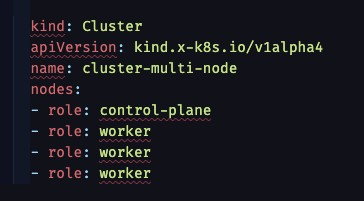
\includegraphics[width=1\textwidth]{resources/appendix/pembuatan-cluster.jpg}
  \caption{Konfigurasi Pembuatan \textit{Kubernetes Cluster} Dengan Kakas \textit{Kind}}
  \label{fig:konfigurasi-pembuatan-cluster}
\end{figure}

\begin{figure}[ht]
  \centering
  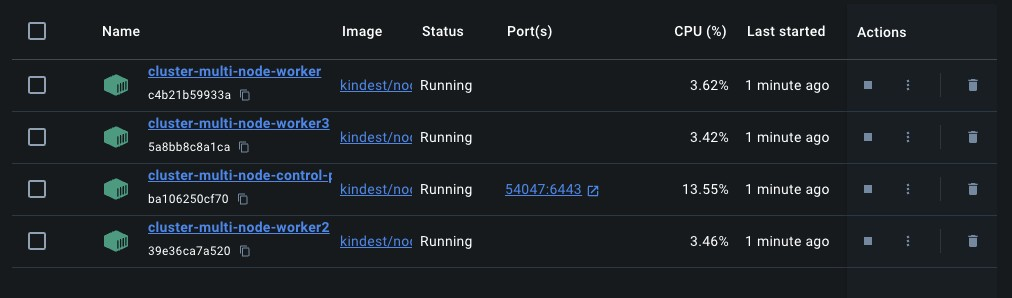
\includegraphics[width=1\textwidth]{resources/chapter-4/cluster-kind.jpg}
  \caption{Hasil \textit{Kubernetes Cluster} Dengan Kakas \textit{Kind}}
  \label{fig:hasil-cluster-kind}
\end{figure}

\pagebreak

\subsection{Implementasi \textit{Dashboard}}
komponen \textit{dashboard} dibuat dengan menggunakan bahasa pemrogramman \textit{typescript} dan \textit{vue}. Framework yang digunakan dalam membuat \textit{Dashboard} adalah \textit{Nuxt}. \textit{Nuxt} menjadi pilihan karena memiliki \textit{developer experience} yang bagus serta fitur yang cukup lengkap. \textit{Nuxt} juga memiliki \textit{UI library} yaitu \textit{NuxtUI} yang memudahkan pembuatan \textit{UI}. Pada komponen ini, terdapat 13 halaman yang dapat dikunjungi oleh \textit{user}. Detail dari penjelasan setiap halaman dapat ditemukan pada subbab dibawah ini.

\subsubsection{Halaman \textit{Login}}
Halaman ini berada pada \textit{route} \textbf{/login}. Halaman ini yang berfungsi sebagai \textit{entrypoint} dari komponen \textit{dashboard}. Pada halaman ini terdapat dua input yang di \textit{wrap} oleh sebuah \textit{form}. Input berupa \textit{email} dan \textit{password} \textit{user}. Setelah \textit{user} memasukan \textit{email} dan \textit{password} yang sesuai, maka akan dilakukan \textit{redirect} ke laman utama untuk menunjukan bahwa \textit{user} berhasil terautentikasi dan menggunakan fungsionalitas \textit{dashboard}. Tampilan halaman ini dapat dilihat pada gambar \ref{fig:halaman-login}

\subsubsection{Halaman utama}
Halaman ini merupakan halaman utama dari komponen \textit{dashboard}. Pada halaman ini \textit{user} dapat melihat status dari masing masing objek mulai dari \textit{deployment}, \textit{device}, \textit{group}, serta \textit{quick actions} untuk menuju halaman terkait.

\subsubsection{Halaman \textit{Account}}
Halaman ini berada pada \textit{route \textbf{/account}}. Halaman ini berfungsi untuk memberikan detail mengenai \textit{company} dari \textit{user}. Informasi \textit{company} ditampilkan pada sebuah \textit{card} yang berada pada tengah halaman. Pada halaman ini juga ditampilkan informasi mengenai daftar \textit{user} yang berada pada \textit{company} yang sama dan ditampilkan dengan sebuah tabel. Tampilan halaman ini dapat dilihat pada gambar \ref{fig:halaman-account}

\subsubsection{Halaman \textit{Device}}
Halaman ini berada pada \textit{route \textbf{/devices}}. Halaman ini berfungsi untuk melakukan manajemen \textit{device} pada satu perusahaan. Halaman ini menunjukan informasi seluruh \textit{device} yang terdaftar pada \textit{company}. Tampilan halaman ini dapat dilihat pada gambar \ref{fig:halaman-device}

Sama seperti halaman \textit{account}, terdapat tombol dengan icon elipsis pada bagian kanan untuk melakukan fungsi seperti melihat detail ataupun menghapus \textit{device} terkait. Apabila \textit{user} menekan tombol \textit{detail} maka user akan diarahkan ke halaman \textbf{/device/:id} sesuai dengan id \textit{device} yang dipilih. Tombol yang dimaksud dapat dilihat pada gambar \ref{fig:halaman-device-actions}

Pada halaman ini terdapat tombol yang dapat ditekan untuk menambahkan \textit{device}. Apabila ditekan akan muncul sebuah modal. Modal ini berisi input yang dapat \textit{user} isi untuk membuat sebuah \textit{device} baru pada sistem. Terdapat validasi pada setiap input, setelah semua validasi dilewati, tombol \textit{submit} akan mengirimkan \textit{request} ke \textit{server} untuk di proses. Tombol yang dimaksud dapat dilihat pada gambar \ref{fig:halaman-device-add}

Akan muncul sebuah notifikasi pada bagian kanan bawah tergantung \textit{response} yang diberikan oleh \textit{server}. Warna hijau menandakan bahwa \textit{response} sukses dan warna \textit{merah} menandakan bahwa terdapat masalah ketika memproses \textit{request}.

\subsubsection{Halaman \textit{Device detail}}
Halaman ini dapat diakses dengan cara mengunjungi \textbf{/devices/:id} dari tombol \textit{detail} pada \textit{actions} yang berada pada halaman \textbf{/devices}. Pada halaman ini \textit{user} dapat menambahkan \textit{device} ke dalam sebuah group dengan menekan tombol \textit{add group}. Halaman dapat dilhat pada gambar \ref{fig:halaman-device-detail}

Modal \textit{add group} akan muncul jika tombol ditekan, modal ini memliki sebuah dropdown yang telah berisi \textit{group} yang tersedia pada sistem. Akan muncul sebuah notifikasi pada bagian bawah kanan untuk menandakan bahwa \textit{request} berhasil di proses oleh server. Warna hijau menandakan sukses dan warna merah menandakan bawhwa \textit{server} belum berhasil memproses permintaan tersebut. Modal dapat dilhat pada gambar \ref{fig:halaman-device-detail-add-group}

Pada halaman ini juga terdapat tombol \textit{delete} yang berada pada pojok kanan atas. Jika \textit{user} memutuskan untuk menghapus \textit{device}, akan muncul sebuah modal konfirmasi sebelum aksi penghapusan dilakukan. Modal dapat dilihat pada gambar \ref{fig:halaman-device-detail-delete}

\subsubsection{Halaman \textit{Groups}}
Halaman ini berada pada \textit{route \textbf{/groups}}. Halaman ini menunjukan informasi mengenai \textit{groups} yang telah terdaftar pada sistem. Informasi ditampilkan dalam bentuk tabel yang berisi detail dari objek \textit{groups}. Halaman dapat dilihat pada gambar \ref{fig:halaman-groups}

Pada tabel terdapat tombol elipsis yang terletak pada bagian kanan dari masing masing \textit{row}. Sama seperti tabel lainnya, tombol ini berfungsi untuk melakukan \textit{action} pada \textit{row}. Aksi yang dapat dilakukan berupa mengakses halaman detail atau menghapus \textit{item} tersebut.

Apabila tombol \textit{detail} dipilh maka \textit{user} akan menuju halaman \textit{group detail}. Apabila tombol \textit{delete} dipilih maka \textit{item} akan dihapus dari sistem dan muncul notifikasi pada bagian bawah yang menandkana bahwa proses berhasil dilakukan. Tombol dapat dilhat pada gambar \ref{fig:halaman-groups-actions}

Pada halaman ini juga \textit{user} dapat menambahkan \textit{groups} dengan menekan tombol \textit{add group}. Ketika tombol ini ditekan akan muncul modal yang memiliki input nama. Input ini memiliki validasi berupa panjang karakter yang dimasukan haruslah memiliki panjang minimal 8 karakter. Setelah validasi berhasil di lewati, maka tombol submit akan berfungsi untuk mengirimkan \textit{request} ke server. Akan muncul notifikasi pada bagian bawah kanan untuk menandakan bahwa \textit{request} berhasil di proses. Warna hijau menandakan bahwa \textit{request} berhasil di proses dan warna merah menandakan sebaliknya. Modal dapat dilihat pada gambar \ref{fig:halaman-groups-add}

\subsubsection{Halaman \textit{Groups detail}}
Halaman ini dapat diakses oleh \textit{pengguna} melalui tombol \textit{detail} yang ada pada tabel di halaman \textit{groups}. Halaman ini memiliki \textit{route \textbf{/groups/:id}}. Pada halaman ini \textit{user} dapat melihat informasi mengenai detail dari \textit{groups} yang dipilih mulai dari nama, deskripsi dan \textit{device} apa saja yang telah terhubung pada \textit{group tersebut}. Halaman dapat dilihat pada \ref{fig:halaman-groups-detail}

\textit{user} juga dapat menambahkan \textit{device} dengan cara menekan tombol \textit{add devices} yang akan memunculkan modal berisi dropdown seluruh perangkat yang belum memiliki \textit{groups}. \textit{Dropdown} dapat dilihat pada gambar \ref{fig:halaman-groups-detail-add-group} dan \ref{fig:halaman-groups-detail-delete}

\subsubsection{Halaman \textit{Deployment}}
Halaman ini merupakan fungsionalitas utama dari sistem \textit{remote deployment}. Halaman ini dapat diakses melalui \textit{sidebar} dan memiliki \textit{route \textbf{/deployments}}. Pada halaman ini \textit{user} dapat melihat informasi mengenai \textit{deployment plan} yang terdaftar pada sistem. Selain itu juga terdapat informasi mengenai \textit{deployment images} yang tersedia dalam sistem. Kedua informasi ditampilkan dalam bentuk tabel yang masing masing memiliki tombol \textit{add} pada bagian kanan bawah tabel. Halaman dapat dilihat pada gambar \ref{fig:halaman-deployment}

Tombol add tersebut akan memunculkan modal yang berisi input yang harus diisi jika ingin membuat \textit{item} baru. Sama seperti tabel lainnya, pada masing masing tabel terdapat tombol elipsis pada bagian kanan untuk melakukan aksi berupa melihat \textit{detail} ataupun menghapus \textit{item} yang bersesuaian. Tampilan tombol dapat dilihat pada gambar \ref{fig:halaman-deployment-add-deployment} dan \ref{fig:halaman-deployment-add-repostory}

\subsubsection{Halaman \textit{deployments detail}}
Halaman ini dapat diakses melalui tombol \textit{detail} di tabel \textit{deployment} pada halaman \textit{deployment}. Halaman ini memiliki \textit{route \textbf{/deployments/:id}}. Halaman ini menunjukan informasi mengenai \textit{deployment} yang telah dilakukan, status dari \textit{deployment}, serta target dari \textit{deployment} tersebut. Tampilan halaman dapat dilihat pada gambar \ref{fig:halaman-deployment-detail}

Pada halaman ini juga terdapat tombol \textit{delete} yang berada pada pojok kanan atas. Dengan menekan tombol ini, akan muncul sebuah modal untuk melakukan konfirmasi jika ingin menghapus \textit{deployment}. Tampilan dapat dilihat pada gambar \ref{fig:halaman-deployment-detail-delete}

\subsubsection{Halaman \textit{FAQ}}
Halaman ini berada pada \textit{route \textbf{/faq}}. Halaman ini bertujuan untuk memberikan informasi mengenai tata cara hal yang perlu dilakukan sebelum mendaftarkan \textit{device} ke sistem. Terdapat dua bagian yang dibedakan dari banyaknya \textit{device} yang terhubung ke dalam sistem. Dua kategori tersebut yaitu jika belum memiliki \textit{device} sama sekali dan memiliki setidaknya 1 \textit{device} yang telah terhubung dengan sistem.


\pagebreak

\subsection{Implementasi \textit{Service}}

Implementasi \textit{service} dibuat dengan menggunakan bahasa pemrogramman golang dan framework \textit{Echo} serta menggunakan \textit{REST API} sebagai gaya komunikasinya. Arsitektur kode yang dibuat memiliki tiga lapisan dimulai dari \textit{handler}, \textit{usecase}, dan \textit{repository}. Handler bertujuan membaca permintaan pengguna dan dapat disebut sebagai entrypoint. Data dari handler akan diberikan kepada \textit{usecase} untuk diproses. \textit{Usecase} merupakan lapisan yang hanya memiliki \textit{logic} proses bisnis. Setelah data berhasil melewati lapisan \textit{usecase}, data siap untuk dimasukkan ke database. Proses hubungan antara \textit{service} dengan \textit{database} diletakan pada lapisan \textit{repository}.

Pemisahan lapisan ini mengikuti design pattern yaitu \textit{dependency injection}. Selain itu, pemisahan ini juga bertujuan memudahkan testing dan meningkatkan \textit{maintanability} karena mudah untuk dibaca dan dipahami. \textit{endpoint} dibuat dengan menggunakan versioning dengan base \textit{endpoint} \textbf{/v1}. Versioning digunakan untuk memudahkan penggantian endpoint jika suatu saat terdapat perubahan major yang bersifat \textit{breaking}. Selain itu base \textit{endpoint} untuk \textit{user} dan \textit{admin} memiliki perbedaan pada prefix \textbf{/api} dan \textbf{/admin-api}

Pada sistem ini terdapat \textit{middleware} yang digunakan untuk melakukan autorisasi \textit{pengguna}. Berikut merupakan daftar dan penjelasan \textit{middleware} pada sistem

\begin{enumerate}
  \item ValidateAPIKey

        \textit{Middleware} ini bertujuan untuk memastikan bahwa hanya \textit{client} yang sesuai lah yang dapat mengakses \textit{service}. API Key dikirimkan dengan cara meletakan pada header dengan key \textbf{X-API-Key}. Middleware ini akan dijalankan untuk seluruh \textit{endpoint} yang ada pada \textit{service}.

  \item ValidateJWTKey

        \textit{Middleware} ini memiliki fungsi untuk memvalidasi JWT ketika \textit{user} mengirimkan \textit{request}. \textit{Middleware} ini dijalankan dengan melakukan parsing \textit{accessToken} yang didapat dari cookie pada setiap \textit{request}. Cookie didapat ketika \textit{user} telah melakukan login sebelumnya dan memiliki batas waktu \textit{expire}. Setelah berhasil \textit{login} \textit{user} akan memiliki dua buah cookie yaitu \textit{accessToken} dan \textit{refreshToken}.  \textit{Middleware} ini berjalan untuk seluruh \textit{endpoint user} kecuali \textit{refresh dan login}


  \item ValidateAdminAPIKey

        \textit{middleware} ini memiliki fungsi untuk melakukan autorisasi \textit{admin}. Terdapat Admin API Key yang dilietakan pada header dari setiap \textit{request} dengan key \textbf{X-Admin-API-Key}. Middleware ini berjalan untuk seluruh \textit{endpoint} dengan prefix \textbf{admin-api}.
\end{enumerate}


\subsubsection{Domain \textit{company}}

Domain ini memiliki 4 \textit{endpoint} dengan deskripsi 1 untuk \textit{user} dan 3 untuk \textit{admin}. \textit{middleware} ValidateJWTKey digunakan pada \textit{endpoint user}. Untuk ketiga \textit{endpoint} admin, menggunakan \textit{middleware} ValidateAdminAPIKey. Implementasi dari domain ini akan dijelaskan untuk setiap fungsi dengan acuan gambar \ref{fig:company-class-diagram} dan pemetaan \textit{endpoint} dapat dilihat pada tabel \ref{tab:api-contract-domain-company}


\bgroup
\begin{table}[ht]
  \caption{Api Contract Domain Company}
  \label{tab:api-contract-domain-company}
  \def\arraystretch{1.7}
  \centering
  \begin{tabular}{|c|p{6cm}|p{4cm}|}
    \hline
    Method & Endpoint                    &
    Fungsi                                                  \\
    \hline
    GET    & /api/v1/companies           & GetCompanyDetail \\
    \hline
    POST   & /admin-api/v1/companies     & Create           \\
    \hline
    GET    & /admin-api/v1/companies     & GetAll           \\
    \hline
    GET    & /admin-api/v1/companies/:id & GetById          \\
    \hline
    DELETE & /admin-api/v1/companies/:id & Delete           \\
    \hline
  \end{tabular}
\end{table}
\egroup

\begin{enumerate}
  \item Create

        Fungsionalitas ini menerima masukan berupa json yang dengan \textit{field} \textit{name} dan \textit{cluster\textunderscore name} dari \textit{requester}. Kedua \textit{field} tersebut digunakan untuk mengidentifikasi cluster dari setiap \textit{company}. Terdapat validasi berupa unique (name, cluster\textunderscore name) pada \textit{databse} untuk memastikan bahwa tidak ada duplikat untuk setiap \textit{company}. Setelah semua validasi selesai \textit{server} akan memberikan \textit{response} berupa objek \textit{company} kepada \textit{requester}. Apabila gagal maka akan diberikan pesan error

  \item GetAll

        Fungsionalitas ini dapat dipanggil tanpa masukan apapun oleh admin. Fungsionalitas ini akan mengembalikan semua \textit{company} yang ada pada \textit{database} lalu mengembalikan kepada \textit{requester}.

  \item GetById

        Fungsionalitas ini dapat diakses oleh admin dengan cara memberikan \textit{company id} pada URL. Fungsi ini akan mencari id yang bersesuaian pada \textit{database} lalu mengembalikannya kepada \textit{requester}. Apabila id yang diberikan tidak valid maka akan dikembalikan pesan error

  \item GetCompanyDetail

        Fungsionalitas ini dapat diakses oleh \textit{user} untuk mendapatkan informasi mengenai \textit{company detail} miliknya. Fungsionalitas ini tidak menerima request apapun namun terdapat validasi jika \textit{companyId} dari \textit{user} tidak valid maka akan diberikan pesan error serta apabila \textit{accessToken} sudah \textit{expire} akan dikeluarkan pesan \textit{unauthorized}

  \item Delete

        Fungsionalitas ini dapat diakses oleh \textit{admin} untuk menghapus \textit{company} dari \textit{database}. Karena \textit{company} memiliki relasi ke banyak domain, ketika \textit{company} di delete akan mengadaptasi sistem \textit{cascade} sehingga seluruh data yang memiliki referensi ke \textit{companyId} akan terhapus secara otomatis.

\end{enumerate}


\subsubsection{Domain \textit{user}}

Domain ini memiliki relasi \textit{one} to \textit{many} dengan domain \textit{company} karena satu company bisa memiliki banyak \textit{user}. Terdapat 7 \textit{endpoint} dengan detail 4 untuk \textit{user} dan 3 untuk \textit{admin}. Implementasi dari domain ini akan dijelaskan untuk setiap fungsi dengan acuan gambar \ref{fig:user-class-diagram} dan pemetaan \textit{endpoint} dapat dilihat pada tabel \ref{tab:api-contract-domain-user}

\bgroup
\begin{table}[ht]
  \caption{Api Contract Domain User}
  \label{tab:api-contract-domain-user}
  \def\arraystretch{1.7}
  \centering
  \begin{tabular}{|c|p{6cm}|p{4cm}|}
    \hline
    Method & Endpoint                &
    Fungsi                                     \\
    \hline
    GET    & /api/v1/users           & GetAll  \\
    \hline
    GET    & /api/v1/users/:id       & GetById \\
    \hline
    POST   & /api/v1/users/login     & Login   \\
    \hline
    POST   & /api/v1/users/refresh   & Refresh \\
    \hline
    GET    & /admin-api/v1/users     & GetAll  \\
    \hline
    POST   & /admin-api/v1/users     & Create  \\
    \hline
    DELETE & /admin-api/v1/users/:id & Delete  \\
    \hline
  \end{tabular}
\end{table}
\egroup


\begin{enumerate}
  \item GetAll

        Fungsionalitas ini dapat dipanggil tanpa masukan apapun. Fungsi ini akan memiliki pengecekan apakah user ataupun admin dan mengembalikan hasil yang sesuai. Jika \textit{user} yang memanggil fungsi ini maka akan dikembalikan user pada satu \textit{company} dan jika \textit{admin} yang memanggil ini maka akan dikembalikan seluruh user yang ada kepada \textit{requester}.

  \item GetById

        Fungsionalitas ini dapat diakses oleh \textit{user} dengan cara memberikan \textit{user id} pada URL. Fungsi ini akan mencari id yang bersesuaian pada \textit{database} lalu mengembalikannya kepada \textit{requester}. Apabila id yang diberikan tidak valid maka akan dikembalikan pesan error

  \item Login

        Fungsionalitas ini menerima masukan berupa json yang dengan \textit{field} \textit{email} dan \textit{password} dari \textit{requester}. Kedua field tersebut akan digunakan untuk mencari \textit{user} yang bersesuaian pada \textit{database}. Setelah data ditemukan akan dilakukan validasi password dengan cara melakukan \textit{compare hash} password dengan hash password yang tersimpan di database. Setelah semua validasi berhasil dilakukan maka, akan dikembalikan response serta cookie yang dengan "accessToken" dan "refreshToken". Apabila gagal maka akan diberikan pesan error

        Kedua cookie ini nantinya akan digunakan untuk mengautorisasi setiap request. "accessToken" memiliki waktu \textit{expire} selama 1 jam dan "refreshToken" memiliki waktu \textit{expire} selama 1 hari. Untuk meningkatkan keamanan dan menghindari CSRF, Cookie di set dengan attribut "httpOnly", "sameSiteLax", serta "secure".

  \item Refresh

        Fungsionalitas ini menerima masukan berupa "refreshToken" dan akan memberikan "accessToken" baru ketika \textit{endpoint} ini di panggil oleh \textit{requester}. "refreshToken" akan \textit{expire} secara otomatis setelah 1 hari sehingga \textit{endpoint} ini otomatis akan mengembalikan pesan error jika "refreshToken" sudah \textit{expire}.

  \item Create

        Fungsionalitas ini menerima masukan berupa json yang dengan \textit{field} \textit{name}, \textit{email}, \textit{password}, serta \textit{company\textunderscore id} dari \textit{requester}. Seluruh \textit{field} tersebut digunakan untuk membuat objek user pada \textit{database}. Pada fungsi ini akan dilakukan pengecekan apakah \textit{email} valid dan \textit{unique}. Selain itu ada validasi \textit{company\textunderscore id} agar dipastikan bahwa \textit{user} benar terdaftar ke \textit{company} yang sesuai. Apabila validasi tidak berhasil maka akan dikeluarkan pesan error, namun jika semua berhasil dilewati maka akan dikembalikan \textit{response} berupa \textit{user} yang telah dibuat pada database.

  \item Delete

        Fungsionalitas ini dapat diakses oleh \textit{admin} untuk menghapus \textit{user} dari \textit{database}. Fungsi ini menerima parameter berupa id dari \textit{user} yang ingin dihapus. Apabila ada \textit{relasi} lain yang mengacu kepada \textit{user}, maka akan mengadpdatasi sistem \textit{cascade} sehingga seluruh data akan ikut terhapus juga.

\end{enumerate}

\subsubsection{Domain \textit{devices}}

Domain ini memiliki relasi \textit{one} to \textit{many} dengan domain \textit{company} karena satu company bisa memiliki banyak \textit{devices}. Terdapat 6 \textit{endpoint} dengan detail 5 untuk \textit{user} dan 1 untuk \textit{admin}. Implementasi dari domain ini akan dijelaskan untuk setiap fungsi dengan acuan gambar \ref{fig:device-class-diagram} dan pemetaan \textit{endpoint} dapat dilihat pada tabel \ref{tab:api-contract-domain-device}

\bgroup
\begin{table}[ht]
  \caption{Api Contract Domain Devices}
  \label{tab:api-contract-domain-device}
  \def\arraystretch{1.7}
  \centering
  \begin{tabular}{|c|p{6cm}|p{4cm}|}
    \hline
    Method & Endpoint                   &
    Fungsi                                                    \\
    \hline
    GET    & /admin-api/v1/devices      & GetAll              \\
    \hline
    GET    & /api/v1/devices            & GetAllByCompanyId   \\
    \hline
    GET    & /api/v1/devices/:id        & GetById             \\
    \hline
    GET    & /api/v1/devices/:id/groups & GetGroupsByDeviceId \\
    \hline
    POST   & /api/v1/devices            & Create              \\
    \hline
    DELETE & /api/v1/devices/:id        & Delete              \\
    \hline
  \end{tabular}
\end{table}
\egroup


\begin{enumerate}
  \item GetAll

        Fungsionalitas ini dapat dipanggil tanpa masukan apapun. Fungsi ini digunakan untuk admin untuk mendapatkan seluruh informasi \textit{device} yang terdaftar pada \textit{database}. Tidak ada validasi dan apabila data kosong maka akan dikembalikan daftar kosong.

  \item GetAllByCompanyId

        Fungsionalitas ini dapat diakses oleh \textit{user} untuk mendapatkan seluruh \textit{device} yang dimiliki oleh \textit{company}. Middleware ValidateJWTKey akan mencoba untuk melakukan \textit{decode} "accessToken" dan mengambil informasi "companyId" dari hasil tersebut. Jika tidak valid maka akan dikeluarkan pesan error. Setelah semua validasi berhasil maka daftar seluruh \textit{device} akan menjadi \textit{repsonse} dan dikembalikan kepada \textit{requester}.

  \item GetById

        Fungsionalitas ini dapat diakses oleh \textit{user} untuk mendapatkan detail dari \textit{device} dengan cara memberikan \textit{id} yang sesuai. Apabila tidak ditemukan maka akan mengeluarkan pesan error.

  \item GetGroupsByDeviceId


        Fungsionalitas ini akan mengembalikan seluruh relasi \textit{groups} yang berkaitan dengan \textit{device id} terkait. Fungsi ini akan menerima \textit{device id} dan akan mencari apakah terdapat \textit{groups} yang berkaitan dengan id tersebut. Fungsi ini akan mengembalikan seluruh \textit{groups} yang ada dan jika tidak ada satupun maka akan dikeluarkan daftar kosong. Apabila \textit{device id} tidak valid maka akan diberikan pesan error.

  \item Create

        Fungsionalitas ini menerima masukan berupa json yang dengan \textit{field} \textit{name}, \textit{type}, \textit{attributes}, serta \textit{node\textunderscore name} dari \textit{requester}. Seluruh \textit{field} tersebut digunakan untuk membuat objek \textit{device} pada \textit{database}. Pada fungsi ini akan dilakukan pengecekan apakah \textit{node\textunderscore name} ada pada \textit{cluster} serta merupakan nama yang valid dan \textit{unique}. Selain itu terdapat validasi \textit{attributes} yaitu merupakan list of string yang masing masing harus memiliki '=' sebagai tanda pemisah. Hal ini dilakukan karena ini merupakan label yang akan diberikan pada \textit{node} pada \textit{cluster} nantinya. Apabila validasi tidak berhasil maka akan dikeluarkan pesan error, namun jika semua berhasil dilewati maka akan dikembalikan \textit{response} berupa \textit{device} yang telah dibuat pada database serta proses \textit{node} pada \textit{cluster} yang sudah di labeli dengan \textit{attributes}.

  \item Delete

        Fungsionalitas ini dapat diakses oleh \textit{user} untuk menghapus \textit{device} dari \textit{database}. Fungsi ini menerima parameter berupa id dari \textit{device} yang ingin dihapus. Apabila ada \textit{relasi} lain yang mengacu kepada \textit{device}, maka akan mengadpdatasi sistem \textit{cascade} sehingga seluruh data akan ikut terhapus juga.

\end{enumerate}

\subsubsection{Domain \textit{groups}}

Domain ini memiliki relasi \textit{one} to \textit{many} dengan domain \textit{company} karena satu \textit{company} bisa memiliki banyak \textit{groups}. Terdapat 6 \textit{endpoint} dengan detail 5 untuk \textit{user} dan 1 untuk \textit{admin}. Implementasi dari domain ini akan dijelaskan untuk setiap fungsi dengan acuan gambar \ref{fig:groups-class-diagram} dan pemetaan \textit{endpoint} dapat dilihat pada tabel \ref{tab:api-contract-domain-groups}

\bgroup
\begin{table}[ht]
  \caption{Api Contract Domain Groups}
  \label{tab:api-contract-domain-groups}
  \def\arraystretch{1.7}
  \centering
  \begin{tabular}{|c|p{6cm}|p{4cm}|}
    \hline
    Method & Endpoint                  &
    Fungsi                                                  \\
    \hline
    GET    & /admin-api/v1/groups      & GetAll             \\
    \hline
    GET    & /api/v1/groups            & GetAllByCompanyId  \\
    \hline
    GET    & /api/v1/groups/:id        & GetById            \\
    \hline
    GET    & /api/v1/groups/:id/groups & GetDeviceByGroupId \\
    \hline
    POST   & /api/v1/groups            & Create             \\
    \hline
    DELETE & /api/v1/groups/:id        & Delete             \\
    \hline
  \end{tabular}
\end{table}
\egroup

\begin{enumerate}
  \item GetAll

        Fungsionalitas ini dapat dipanggil tanpa masukan apapun. Fungsi ini digunakan untuk admin untuk mendapatkan seluruh informasi \textit{groups} yang terdaftar pada \textit{database}. Tidak ada validasi dan apabila data kosong maka akan dikembalikan daftar kosong.

  \item GetAllByCompanyId

        Fungsionalitas ini dapat diakses oleh \textit{user} untuk mendapatkan seluruh \textit{groups} yang dimiliki oleh \textit{company}. Middleware ValidateJWTKey akan mencoba untuk melakukan \textit{decode} "accessToken" dan mengambil informasi "companyId" dari hasil tersebut. Jika tidak valid maka akan dikeluarkan pesan error. Setelah semua validasi berhasil maka daftar seluruh \textit{groups} akan menjadi \textit{repsonse} dan dikembalikan kepada \textit{requester}.

  \item GetById

        Fungsionalitas ini dapat diakses oleh \textit{user} untuk mendapatkan detail dari \textit{groups} dengan cara memberikan \textit{id} yang sesuai. Apabila tidak ditemukan maka akan mengeluarkan pesan error.

  \item GetDeviceByGroupId


        Fungsionalitas ini akan mengembalikan seluruh relasi \textit{device} yang berkaitan dengan \textit{group id} terkait. Fungsi ini akan menerima \textit{group id} dan akan mencari apakah terdapat \textit{device} yang berkaitan dengan id tersebut. Fungsi ini akan mengembalikan seluruh \textit{device} yang ada dan jika tidak ada satupun maka akan dikeluarkan daftar kosong. Apabila \textit{group id} tidak valid maka akan diberikan pesan error.

  \item Create

        Fungsionalitas ini menerima masukan berupa json yang dengan \textit{field} \textit{name}. \textit{Field name} memiliki \textit{unique constraint} sehingga tidak mungkin ada nama \textit{groups} yang sama pada satu \textit{company}. Terdapat validasi untuk membuat nama \textit{groups} yang memiliki panjang minimal 8 characters untuk menghindari memberikan nama tanpa konteks. Apabila terdapat duplikat maka akan dikembalikan pesan error dan setelah semua validasi berhasil, \textit{service} akan mengirimkan \textit{response} berupa \textit{groups} yang berhasil dibuat kepada \textit{requester}.

  \item Delete

        Fungsionalitas ini dapat diakses oleh \textit{user} untuk menghapus \textit{groups} dari \textit{database}. Fungsi ini menerima parameter berupa id dari \textit{groups} yang ingin dihapus. Apabila ada \textit{relasi} lain yang mengacu kepada \textit{groups}, maka akan mengadpdatasi sistem \textit{cascade} sehingga seluruh data akan ikut terhapus juga.

\end{enumerate}


\subsubsection{Domain \textit{deployment}}

Domain ini memiliki relasi \textit{one} to \textit{one} dengan domain \textit{external service}. Selain itu domain ini juga memiliki relasi one to many dengan \textit{company}. Karena satu \textit{company} bisa memiliki banyak \textit{deployment}. Pada domain ini akan dibagi menjadi tiga bagian yaitu \textit{deployment images}, \textit{deployment histories} dan \textit{deployment}. Hubungan domain dapat dilihat pada gambar \ref{fig:deployment-class-diagram}

\subsubsubsection{Deployment Images}
Pada bagian ini yang terdapat 5 \textit{endpoint} dengan detail 4 untuk \textit{user} dan 1 untuk \textit{admin}. Implementasi dari domain ini akan dijelaskan untuk setiap fungsi dengan acuan gambar \ref{fig:deployment-class-diagram} dan pemetaan \textit{endpoint} dapat dilihat pada tabel \ref{tab:api-contract-domain-deployment-images}

\bgroup
\begin{table}[ht]
  \caption{Api Contract Domain Deployment Images}
  \label{tab:api-contract-domain-deployment-images}
  \def\arraystretch{1.7}
  \centering
  \begin{tabular}{|c|p{6cm}|p{4cm}|}
    \hline
    Method & Endpoint                   &
    Fungsi                                                  \\
    \hline
    GET    & /admin-api/v1/repositories & GetAll            \\
    \hline
    GET    & /api/v1/repositories       & GetAllByCompanyId \\
    \hline
    GET    & /api/v1/repositories/:id   & GetById           \\
    \hline
    POST   & /api/v1/repositories       & Create            \\
    \hline
    DELETE & /api/v1/repositories/:id   & Delete            \\
    \hline
  \end{tabular}
\end{table}
\egroup


\begin{enumerate}
  \item GetAll

        Fungsionalitas ini dapat dipanggil tanpa masukan apapun. Fungsi ini digunakan untuk admin untuk mendapatkan seluruh informasi \textit{deployment images} yang terdaftar pada \textit{database}. Tidak ada validasi dan apabila data kosong maka akan dikembalikan daftar kosong.

  \item GetAllByCompanyId

        Fungsionalitas ini dapat diakses oleh \textit{user} untuk mendapatkan seluruh \textit{deployment images} yang dimiliki oleh \textit{company}. Middleware ValidateJWTKey akan mencoba untuk melakukan \textit{decode} "accessToken" dan mengambil informasi "companyId" dari hasil tersebut. Jika tidak valid maka akan dikeluarkan pesan error. Setelah semua validasi berhasil maka daftar seluruh \textit{deployment images} akan menjadi \textit{repsonse} dan dikembalikan kepada \textit{requester}.

  \item GetById

        Fungsionalitas ini dapat diakses oleh \textit{user} untuk mendapatkan detail dari \textit{deployment images} dengan cara memberikan \textit{id} yang sesuai. Apabila tidak ditemukan maka akan mengeluarkan pesan error.

  \item Create

        Fungsionalitas ini menerima masukan berupa json yang dengan \textit{field} \textit{name}, \textit{description}, \textit{image}. Teradapat \textit{unique constraint} pada \textit{field nama dan image} pada satu \textit{company} untuk mencegah duplikat. Apabila terdapat duplikat maka akan dikembalikan pesan error dan setelah semua validasi berhasil, \textit{service} akan mengirimkan \textit{response} berupa \textit{deployment images} yang berhasil dibuat kepada \textit{requester}.

  \item Delete

        Fungsionalitas ini dapat diakses oleh \textit{user} untuk menghapus \textit{eployment images} dari \textit{database}. Fungsi ini menerima parameter berupa id dari \textit{eployment images} yang ingin dihapus. Apabila ada \textit{relasi} lain yang mengacu kepada \textit{eployment images}, maka akan mengadpdatasi sistem \textit{cascade} sehingga seluruh data akan ikut terhapus juga.

\end{enumerate}

\subsubsubsection{Deployment Histories}
Pada bagian ini yang terdapat 5 \textit{endpoint} dengan detail 4 untuk \textit{user} dan 1 untuk \textit{admin}. Implementasi dari domain ini akan dijelaskan untuk setiap fungsi dengan acuan gambar \ref{fig:deployment-class-diagram} dan pemetaan \textit{endpoint} dapat dilihat pada tabel \ref{tab:api-contract-domain-deployment-histories}

\bgroup
\begin{table}[ht]
  \caption{Api Contract Domain Deployment Histories}
  \label{tab:api-contract-domain-deployment-histories}
  \def\arraystretch{1.7}
  \centering
  \begin{tabular}{|c|p{6cm}|p{4cm}|}
    \hline
    Method & Endpoint                &
    Fungsi                                               \\
    \hline
    GET    & /admin-api/v1/histories & GetAll            \\
    \hline
    GET    & /api/v1/histories       & GetAllByCompanyId \\
    \hline
    GET    & /api/v1/histories/:id   & GetById           \\
    \hline
    POST   & /api/v1/histories       & Create            \\
    \hline
    DELETE & /api/v1/histories/:id   & Delete            \\
    \hline
  \end{tabular}
\end{table}
\egroup


\begin{enumerate}
  \item GetAll

        Fungsionalitas ini dapat dipanggil tanpa masukan apapun. Fungsi ini digunakan untuk admin untuk mendapatkan seluruh informasi \textit{deployment histories} yang terdaftar pada \textit{database}. Tidak ada validasi dan apabila data kosong maka akan dikembalikan daftar kosong.

  \item GetAllByCompanyId

        Fungsionalitas ini dapat diakses oleh \textit{user} untuk mendapatkan seluruh \textit{deployment histories} yang dimiliki oleh \textit{company}. Middleware ValidateJWTKey akan mencoba untuk melakukan \textit{decode} "accessToken" dan mengambil informasi "companyId" dari hasil tersebut. Jika tidak valid maka akan dikeluarkan pesan error. Setelah semua validasi berhasil maka daftar seluruh \textit{deployment histories} akan menjadi \textit{repsonse} dan dikembalikan kepada \textit{requester}.

  \item GetById

        Fungsionalitas ini dapat diakses oleh \textit{user} untuk mendapatkan detail dari \textit{deployment histories} dengan cara memberikan \textit{id} yang sesuai. Apabila tidak ditemukan maka akan mengeluarkan pesan error.

  \item Create

        Fungsionalitas ini menerima masukan berupa json yang dengan \textit{field} \textit{device\textunderscore id}, \textit{repository\textunderscore id}, \textit{deployment\textunderscore id}. Tidak ada validasi ketika ingin membuat \textit{deployement histories} dan \textit{Service} mengirimkan \textit{response} berupa \textit{deployment histories} yang berhasil dibuat kepada \textit{requester}.

  \item Delete

        Fungsionalitas ini dapat diakses oleh \textit{user} untuk menghapus \textit{eployment histories} dari \textit{database}. Fungsi ini menerima parameter berupa id dari \textit{deployment histories} yang ingin dihapus. Apabila ada \textit{relasi} lain yang mengacu kepada \textit{deployment histories}, maka akan mengadpdatasi sistem \textit{cascade} sehingga seluruh data akan ikut terhapus juga.

\end{enumerate}

\subsubsubsection{Deployment plan}
Pada bagian ini yang terdapat 7 \textit{endpoint} dengan detail 6 untuk \textit{user} dan 1 untuk \textit{admin}. Implementasi ini merupakan implementasi utama dari domain ini. Bagian ini juga menjadi terhubung dengan dua bagian lainnya serperti pada gambar \ref{fig:deployment-class-diagram}. Pemetaan \textit{endpoint} dapat dilihat pada tabel \ref{tab:api-contract-domain-deployment}

\bgroup
\begin{table}[ht]
  \caption{Api Contract Domain Deployment plan}
  \label{tab:api-contract-domain-deployment}
  \def\arraystretch{1.7}
  \centering
  \begin{tabular}{|c|p{6cm}|p{4cm}|}
    \hline
    Method & Endpoint                          &
    Fungsi                                                         \\
    \hline
    GET    & /admin-api/v1/deployments         & GetAll            \\
    \hline
    GET    & /api/v1/deployments               & GetAllByCompanyId \\
    \hline
    GET    & /api/v1/deployments/:id           & GetById           \\
    \hline
    POST   & /api/v1/deployments               & Create            \\
    \hline
    DELETE & /api/v1/deployments/:id           & Delete            \\
    \hline
    POST   & /api/v1/deployments/deploy        & Deploy            \\
    \hline
    POST   & /api/v1/deployments/deploy/delete & DeleteDeploy      \\
    \hline
  \end{tabular}
\end{table}
\egroup


\begin{enumerate}
  \item GetAll

        Fungsionalitas ini dapat dipanggil tanpa masukan apapun. Fungsi ini digunakan untuk admin untuk mendapatkan seluruh informasi \textit{deployment plan} yang terdaftar pada \textit{database}. Tidak ada validasi dan apabila data kosong maka akan dikembalikan daftar kosong.

  \item GetAllByCompanyId

        Fungsionalitas ini dapat diakses oleh \textit{user} untuk mendapatkan seluruh \textit{deployment plan} yang dimiliki oleh \textit{company}. Middleware ValidateJWTKey akan mencoba untuk melakukan \textit{decode} "accessToken" dan mengambil informasi "companyId" dari hasil tersebut. Jika tidak valid maka akan dikeluarkan pesan error. Setelah semua validasi berhasil maka daftar seluruh \textit{deployment plan} akan menjadi \textit{repsonse} dan dikembalikan kepada \textit{requester}.

  \item GetById

        Fungsionalitas ini dapat diakses oleh \textit{user} untuk mendapatkan detail dari \textit{deployment plan} dengan cara memberikan \textit{id} yang sesuai. Apabila tidak ditemukan maka akan mengeluarkan pesan error.

  \item Create

        Fungsionalitas ini menerima masukan berupa json yang dengan \textit{field} \textit{name}, \textit{version}, \textit{target}, dan \textit{repository\textunderscore id}. Terdapat validasi yaitu \textit{unique constraint} pada \textit{name, version, dan repository\textunderscore id} pada satu company yang sama untuk mencegah data duplikat yang membingungkan. Setelah validasi selsai maka \textit{Service} mengirimkan \textit{response} berupa \textit{deployment plan} yang berhasil dibuat kepada \textit{requester}. Apabila gagal maka akan dikirimkan pesan error.

  \item Delete

        Fungsionalitas ini dapat diakses oleh \textit{user} untuk menghapus \textit{deployment plan} dari \textit{database}. Fungsi ini menerima parameter berupa id dari \textit{deployment plan} yang ingin dihapus. Apabila ada \textit{relasi} lain yang mengacu kepada \textit{deployment plan}, maka akan mengadpdatasi sistem \textit{cascade} sehingga seluruh data akan ikut terhapus juga.

  \item Deploy

        Fungsionalitas ini merupakan fungsionalitas utama dalam sistem \textit{remote deployment}. Fungsionalitas ini dapat diakses oleh \textit{user} untuk melakukan \textit{remote deployment} sesuai dengan \textit{deployment plan} yang dipilih. Fungsi ini menerima \textit{argument} berupa daftar dari \textit{deployment plan} yang ingin dipilh. Apabila terdapat salah satu \textit{deployment plan} yang tidak ditemukan maka proses akan gagal. Setelah semua validasi berhasil dilakukan, fungsi ini akan melanjutkan untuk memanggil \textit{extenral service kubernetes controller} dengan data yang telah disesuaikan.

  \item DeleteDeploy

        Fungsionalitas ini dapat diakses oleh \textit{user} untuk melakukan \textit{rollback deployment} dari \textit{deployment plan} yang dipilih. Fungsi ini menerima \textit{argument} berupa daftar dari \textit{deployment plan} yang ingin dihapus atau dilakukan \textit{rollback}. Apabila terdapat salah satu \textit{deployment plan} yang tidak ditemukan maka proses akan gagal

\end{enumerate}

\subsubsection{Domain \textit{external services}}

Domain ini memiliki relasi \textit{one} to \textit{one} dengan domain \textit{deployment}. Pada \textit{domain} ini tidak terdapat endpoint karena seluruh \textit{Fungsionalitas} ini akan digunakan pada domain \textit{deployment} pada lapisan \textit{usecase}. Implementasi dari domain ini akan dijelaskan untuk setiap fungsi dengan acuan gambar \ref{fig:kubernetes-controller-class-diagram}.


\begin{enumerate}
  \item GetConfig

        Fungsionalitas ini digunakan untuk mendapatkan \textit{config} dari \textit{kubernetes client} yang dipakai.

  \item GetNodes

        Fungsionalitas ini digunakan untuk mendapatkan seluruh \textit{nodes} yang ada pada \textit{cluster} yang sedang terhubung

  \item SwitchCluster

        Fungsionalitas ini digunakan untuk merubah \textit{koneksi cluster kubernetes} yang digunakan. Karena setiap \textit{company} punya \textit{cluster\textunderscore name} yang berbeda beda maka ketika terdapat \textit{company} yang berbeda yang ingin memproses \textit{deployment} maka domain ini dapat melakukan manajemen \textit{cluster} yang terhubung.

  \item LabelNode

        Fungsionalitas ini digunakan untuk membuat label pada \textit{node} di \textit{cluster}. Label haruslah berbentuk key value yang dipisahkan dengan tanda =. Apabila label tidak valid maka akan mengembalikan error.

  \item Deploy

        Fungsionalitas ini digunakan untuk melakukan deployment pada \textit{cluster}. Deployment dilakukan dengan menargetkan \textit{device} sesuai dengan \textit{field target} pada \textit{deployment plan}. Apabila deployment sudah pernah dibuat, maka akan mengeluarkan pesan error dan jika belum maka proses deployment akan dilaksanakan dan diberikan \textit{response} berupa hasil \textit{deployment}

  \item Get

        Fungsionalitas ini digunakan untuk melakukan melihat seluruh deployment yang telah dibuat pada \textit{cluster} beserta status nya.



  \item Patch

        Fungsionalitas ini digunakan untuk \textit{mengupdate} deployment yang telah dibuat pada \textit{cluster}.

  \item Delete

        Fungsionalitas ini digunakan untuk menghapus \textit{deployment} pada \textit{cluster}.

\end{enumerate}

\pagebreak

\section{Pengujian}
\label{sec:pengujian}


Tujuan dari pengujian ialah untuk memastikan apakah seluruh kebutuhan fungsional dan non-fungsional dari sistem telah terpenuhi.
Untuk pengujian kebutuhan fungsional, pengujian dibagi menjadi dua bagian yaitu pengujian yang dilakukan per komponen lalu dilanjutkan dengan pengujian sistem. Setiap skenario pengujian dijelaskan tujuannya, skenario yang dilakukan, dan hasil pengujian yang didapatkan. Skenario pengujian akan memiliki ID dengan awalan P diikuti dengan dua angka. Seluruh pemetaan pengujian terdapat pada lampiran \ref{chapter:tabel-pengujian}

\subsection{Batasan Pengujian}
\label{subsec:batasan-pengujian}
Berikut adalah batasan yang ditetapkan dalam melakukan pengujian \textit{sistem remote deployment}.

\begin{enumerate}
  \item Pengujian dilakukan di tiga kluster yang berbeda
        \begin{enumerate}
          \item Kubernetes lokal \textit{cluster}
          \item \textit{Google Cloud Platform (GCP) Compute Engine} Kubernetes \textit{cluster}
          \item RaspberryPi Cluster
        \end{enumerate}
  \item Setiap \textit{cluster} memiliki jumlah node yang sama yaitu 2.
  \item \textit{Cluster} dibuat dengan distribusi kubernetes k3s.
  \item Sistem \textit{remote deployment} dijalankan pada komputer lokal yang memilki spesifikasi yang telah dijelaskan pada bagian \ref{sec:lingkungan-implementasi}.
  \item Untuk beberapa fungsionalitas admin digunakan \textit{HTTP Client} yaitu Postman untuk membuat \textit{request} kepada \textit{service}
  \item Cluster sudah tersedia dan siap diakses.
  \item Setiap \textit{request} akan memiliki header X-Api-Key.
  \item Setiap \textit{request} yang mengarah ke /admin-api/ akan memiliki \textit{header} berupa X-Admin-API-Key.
  \item Database sudah terisi sebagian untuk memudahkan proses pengujian.
\end{enumerate}

\subsection{Persiapan Pengujian}
Pada proses pengujian, terdapat tiga lingkungan pengujian yang digunakan untuk menguji sistem \textit{remote deployment}. Ketiga lingkungan tersebut yaitu kubernetes \textit{cluster} lokal, kubernetes \textit{cluster} yang terdapat di \textit{Cloud (GCP)}, serta \textit{cluster} pada RaspberryPi. Ketiga \textit{cluster} ini memiliki jumlah node yang berbeda sesuai dengan penjelasan pada \ref{subsec:batasan-pengujian}.

\subsubsection{Kubernetes Lokal}
Untuk pengujian pada kubernetes lokal, dilakukan pembuatan \textit{cluster} dengan kakas kind untuk membuat cluster yang bernama \textit{testing-cluster-two-nodes} yang memiliki 2 node. Konfigurasi pembuatan sama seperti konfigurasi pada bagian \ref{subsec:persiapan-kubernetes-cluster} hanya saja jumlah nodes yang digunakan yaitu 2.
Karena nodes berjumlah dua maka terdapat 1 \textit{master nodes} dan 1 \textit{slave} node pada \textit{cluster}. Konfigurasi pembuatan cluster dapat dilihat pada gambar \ref{fig:kubernetes-lokal-config-testing}.

\begin{figure}[ht]
  \centering
  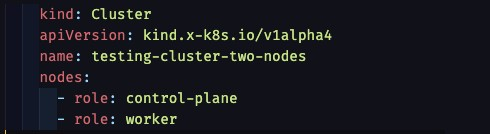
\includegraphics[width=1\textwidth]{resources/chapter-4/pengujian/kubernetes-lokal-config.jpg}
  \caption{Konfigurasi Pembuatan \textit{Kubernetes Testing Cluster} Dengan Kakas \textit{Kind}}
  \label{fig:kubernetes-lokal-config-testing}
\end{figure}

Setelah itu jalankan perintah "kind create cluster --config testing-cluster.yaml" untuk membuat \textit{cluster} pada \textit{docker}. Hasil dari perintahh ini yaitu tercipta dua buah \textit{container} pada \textit{docker} yang memiliki peran \textit{master} dan \textit{slave} seperti pada gambar \ref{fig:kubernetes-lokal-config-testing-result}.

\begin{figure}[ht]
  \centering
  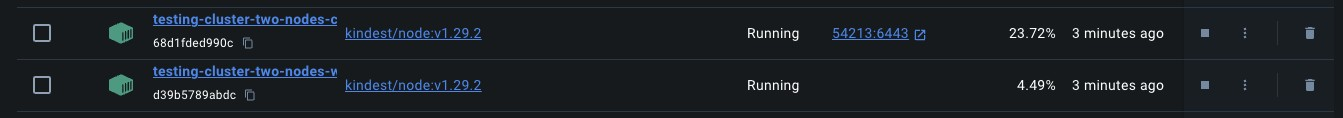
\includegraphics[width=1\textwidth]{resources/chapter-4/pengujian/kubernetes-lokal-config-result.jpg}
  \caption{Hasil \textit{Kubernetes Testing Cluster} pada \textit{Docker}}
  \label{fig:kubernetes-lokal-config-testing-result}
\end{figure}

\subsubsection{Kubernetes GCP}
\label{subsubsec:kubernetes-gcp}
Pada lingkungan ini dibuat dua buah \textit{compute engine (virtual machine)} pada \textit{GCP}. Masing masing dari \textit{virtual machine} akan berperan sebagai kubernetes \textit{cluster} yang bernama \textit{prod-cluster-example}.

\begin{enumerate}
  \item Buat dua \textit{virtual machine} pada \textit{compute engine GCP} dengan spesifikasi berikut. Hasil pembuatan \textit{virtual machine} dapat dilihat pada gambar \ref{fig:hasil-pembuatan-virtual-machine-gcp}
        \begin{enumerate}
          \item Ubuntu 24.04
          \item 2GB Memory
          \item 10GB Storage Persistent Disk
          \item 0.5 - 2Vcpu (1 shared core)
          \item Region Asia southeast2-c
        \end{enumerate}
  \item Membuat \textit{Firewall Rule} Untuk membuka port yang digunakan oleh \textit{kubernetes}. Untuk daftar opsi setiap port yang dibuka dapat dilihat pada gambar \ref{fig:daftar-kegunaan-port}. Untuk hasil pembuatan firewall dapat dilihat pada bagian \ref{fig:hasil-firewall-rule-pada-gcp}
  \item Konfigurasi \textit{gare-test-kubernetes-server} sebagai master nodes. Konfigurasi dilakukan dengan cara mengunduh instalasi dari k3s dengan perintah seperti pada gambar \ref{fig:instalasi-master-node-gcp}.
  \item Konfigurasi virutal machine lainnya yaitu \textit{gare-test-kubernetes-server-node} sebagai \textit{worker node}. Untuk meregistrasi \textit{node} ke dalam \textit{cluster} perlu adanya autentikasi untuk memasitikan hanya \textit{node} yang benar yang boleh masuk ke dalam \textit{cluster}. K3s memiliki token generator yang dapat digunakan untuk mencegah akses yang tidak diinginkan, registrasi token dapat dilihat pada gambar \ref{fig:pengambilan-token-registrasi-cluster}. Token tersebut akan digunakan untuk meregistrasi \textit{node} ini ke \textit{master} dengan \textit{public ip} node tersebut. Ilustrasi dapat dilihat pada gambar \ref{fig:instalasi-worker-node-gcp}.
  \item Ambil konfigurasi \textit{cluster} di \textit{master node} dan pindahkan ke lokasi \textit{server berjalan} untuk meregistrasi \textit{cluster} ke dalam sistem. Setelah melakukan kelima langkah ini \textit{cluster} sudah terintegrasi dengan sistem. Ilustrasi pemindahan konfigurasi dapat dilihat pada gambar \ref{fig:konfigurasi-cluster-master-node-gcp} dan \ref{fig:proses-pemindahan-konfigurasi-master-gcp}.
\end{enumerate}

\subsubsection{Kubernetes RaspberryPi}
Pada lingkungan ini dibuat cluster dengan dua nodes pada RaspberryPi. Cluster yang dibuat bernama cluster-raspi yang memiliki spesifikasi hardware RaspberryPi berikut.

\begin{enumerate}
  \item Master node menggunakan Raspberry Pi 3 Model B Rev 1.2 dengan 1GB RAM dan 4 CPU @ 1.2GHz dengan hostname masterpi. Informasi lebih lengkap dapat dilihat pada gambar \ref{fig:hostname-raspi-master-nodes} dan \ref{fig:spesifikasi-raspi-master-nodes}
  \item Worker node menggunakan Raspberry Pi 2 Model B Rev 1.1 dengan 1GB RAM dan 4 CPU @ 900MHz dengan hostname raspberrypi. Informasi lebih lengkap dapat dilihat pada gambar \ref{fig:hostname-raspi-worker-nodes} dan \ref{fig:spesifikasi-raspi-worker-nodes}
\end{enumerate}

Berikut merupakan tata cara pembuatan cluster kubernetes pada \textit{RaspberryPi}. Diasumsikan \textit{device} \textit{RaspberryPi} sudah terhubung ke dalam jaringan yang sama sehingga tidak perlu \textit{port forwarding} / \textit{public ip}.

\begin{enumerate}
  \item Konfigurasi \textit{hostname masterpi} sebagai master nodes. Perlu dilakukan konfigurasi tambahan untuk menambahkan \textit{cgroups} pada raspberrypi karena secara default opsi ini \textit{disabled}. \textit{Cgroups} merupakan kepanjangan dari \textit{Control Groups} yang berfungsi sebagai \textit{resource management} pada linux dan digunakan dalam proses kontainerisasi. Selanjutnya mirip serperti konfigurasi pada bagian \ref{subsubsec:kubernetes-gcp}, perlu mengunduh instalasi dari k3s dengan perintah seperti pada gambar \ref{fig:instalasi-master-raspi-nodes}.
  \item Konfigurasi \textit{node} lainnya yaitu \textit{hostname raspberrypi} sebagai \textit{worker node}. Untuk meregistrasi \textit{node} ke dalam \textit{cluster} perlu adanya autentikasi untuk memasitikan hanya \textit{node} yang benar yang boleh masuk ke dalam \textit{cluster}. K3s memiliki token generator yang dapat digunakan untuk mencegah akses yang tidak diinginkan, registrasi token dapat dilihat pada gambar \ref{fig:raspi-master-gen-token}. Token tersebut akan digunakan untuk meregistrasi \textit{node} ini ke \textit{master} dengan \textit{ip local} node master. Ilustrasi dapat dilihat pada gambar \ref{fig:instalasi-worker-raspi-node}.
  \item Ambil konfigurasi \textit{cluster} di \textit{master node} dan pindahkan ke lokasi \textit{server berjalan} untuk meregistrasi \textit{cluster} ke dalam sistem. Setelah melakukan langkah ini \textit{cluster} sudah terintegrasi dengan sistem. Ilustrasi pemindahan konfigurasi dapat dilihat pada gambar \ref{fig:raspi-kube-config} dan \ref{fig:raspi-add-kubeconfig}.
\end{enumerate}

\subsection{Pengujian Komponen}
Pengujian di level komponen memastikan bahwa seluruh fungsionalitas yang tidak melibatkan servis eksternal di dalam komponen bekerja dengan baik. Pengujian ini akan dibagi menjadi beberapa bagian sesuai dengan domain yang telah dijelaskan pada bagian \ref{subsec:implementasi-service}. Pada masing masing domain terdapat tabel yang memetakan hubungan antara kebutuhan fungsional serta pengujian yang bersesuaian.

\input{chapters/chapter-4/pengujian/02-01-domain-company.tex}
\input{chapters/chapter-4/pengujian/02-02-domain-user.tex}
\input{chapters/chapter-4/pengujian/02-03-domain-devices.tex}
\input{chapters/chapter-4/pengujian/02-04-domain-groups.tex}
\input{chapters/chapter-4/pengujian/02-05-domain-deployment.tex}
\input{chapters/chapter-4/pengujian/02-06-domain-external.tex}

\subsection{Pengujian Sistem}

\input{chapters/chapter-4/pengujian/03-01-pengujian-sistem-raspi.tex}

\subsection{Pengujian Non Fungsional}
Pada bagian ini, dilakukan pengujian terhadap kebutuhan non-fungsional sistem. Terdapat tiga kebutuhan nonfungsional mulai dari \textit{Security dan Portability}.

\subsubsection{Security}
Pengujian kebutuhan non-fungsional ini dilakukan dengan cara mencoba mengakses \textit{dashboard} dan \textit{service} tanpa meletakan token authentikasi. Bilang yang mau diuji dua aspek ini muali dari auth dan authorization

\begin{enumerate}
  \item Mengakses \textit{dashboard} tanpa kredensial

        Ketika mengakses \textit{dashboard} tanpa memiliki kredensial, \textit{dashboard} memiliki \textit{middleware} yang akan mengecek token yang disimpan pada \textit{client}. Jika token tidak valid maka sistem akan langsung melakukan \textit{redirect} ke halaman login.

  \item Mengakses user \textit{service} tanpa kredensial

        Ketika mencoba untuk mengakses \textit{service} pada endpoint apapun, \textit{service} memiliki \textit{middleware}
        yang akan mengecek header authentikasi yang dikirimkan oleh client. Jika kredensial pada header tidak dicantumkan maka akan mengembalikan \textit{401 Unauthorized} \ref{fig:akses-service-user}

  \item Mengakses admin \textit{service} tanpa kredensial

        Admin endpoint memiliki \textit{middleware} validateAdminJWTKey. Ketika mencoba untuk mengakses \textit{endpoint} admin tanpa memberikan header X-Admin-Api-Key yang sesuai maka \textit{service} akan mengembalikan \textit{401 Unauthorized} seperti pada lampiran \ref{fig:akses-service-admin}

  \item Mengakses \textit{url kubernetes} tanpa kredensial

        Seluruh cluster kubernetes akan mengexpose endpoint pada port 6443. Pengujian ini akan mengakses url kubernetes yaitu https://34.101.95.240:6443/. Ketika diakses, hasilnya akan menunjukan status \textit{401 Unauthorized} seperti pada lampiran \ref{fig:akses-service-kubernetes}

\end{enumerate}

\subsubsection{Portability}
Pengujian kebutuhan non-fungsional ini dialkukan dengan dua skenario yaitu mengakses \textit{dashboard} dari mobile serta mengakses dari berbagai \textit{browser}.

Portability tidak

\begin{enumerate}
  \item Mengakses \textit{dashboard} dari perangkat mobile

        \textit{dashboard} berhasil diakses melalui perangkat mobile dan dapat dilihat hasil dapat dilihat pada lampiran \ref{fig:akses-dashboard-mobile}.

  \item Mengakses \textit{dashboard} dari Chromium based browser

        \textit{dashboard} berhasil diakses melalui browser safari yang dapat dilhat pada lampiran \ref{fig:akses-dashboard-chromium}.

  \item Mengakses \textit{dashboard} dari browser safari

        \textit{dashboard} berhasil diakses melalui browser chromium based yaitu Arc yang dapat dilhat pada lampiran \ref{fig:akses-dashboard-safari}.

\end{enumerate}


% \chapter{Penutup}

Bab Kesimpulan dan Saran akan menjadi bagian akhir dan penutup dari penelitian tugas akhir ini. Bab ini akan membahas kesimpulan yang berisi ketercapaian tujuan penelitian tugas akhir dengan permasalahan yang diselesaikan dalam penelitian tugas akhir. Selain itu, bab ini akan membahas saran yang dapat dilakukan untuk pengembangan atau penelitian selanjutnya.

\section{Kesimpulan}
Penelitian tugas akhir ini mengimplementasikan cara untuk melakukan \textit{remote deployment} pada lingkungan IoT dengan menggunakan kubernetes. Setelah dilakukan analisis, implementasi, dan pengujian, dapat diambil kesimpulan sebagai berikut.
\begin{enumerate}
  \item Sistem \textit{remote deployment} dengan Kubernetes berhasil dibuat dengan arsitektur yang tersentralisasi untuk mengatur proses \textit{remote deployment} pada lingkungan IoT maupun non IoT. Sistem sudah dibuat dengan baik dan berhasil untuk memenuhi kebutuhan fungsional yang telah didefinisikan sebelumnya, namun memiliki \textit{single point of failure} karena arsitektur yang terpusat.
  \item Dengan sistem \textit{remote deployment}, perusahaan dapat dengan mudah untuk melakaukan manajemen perangkat IoT dan melakukan \textit{deployment} dengan mudah.
  \item Kubernetes sudah cocok sebagai \textit{resource manager} yang dipakai untuk proses \textit{remote deployment} pada sistem ini. Dengan seluruh fungsionalitasnya, kubernetes dapat memudahkan dalam proses manajemen perangkat, group, serta \textit{deployment plan}.
\end{enumerate}

\section{Saran}
Adapun banyak kekurangan dan kelemahan yang ditemukan dalam penelitian tugas akhir ini. Berikut adalah beberapa saran yang dapat dilakukan untuk pengembangan atau penelitian selanjutnya.
\begin{enumerate}
  \item Dapat diimplementasikan versioning pada deployment ketika melakukan \textit{rollback}. Ketika versi yang dicapai sudah tidak lagi ditemukan barulah \textit{deployment} di hapus dari \textit{cluster}.
  \item Dapat diimplementasikan	extit{dashboard}untuk \textit{admin} agar memudahkan proses manajemen \textit{company} dan \textit{user}.
  \item Dapat membuat proses \textit{remote deployment} lebih terkustomisasi dengan cara membuat \textit{deployment plan} lebih \textit{flexible} lagi.
  \item Menambahkan fitur seperti \textit{remote command} untuk melakukan eksekusi \textit{command} di setiap perangkat tanpa harus melakukannya satu persatu
  \item Proses registrasi \textit{node} pada \textit{cluster} masih dilakukan secara manual, dapat digunakan sistem \textit{device discovery} untuk mengeleminasi proses yang redundan.
  \item Sistem dapat dibuat sebagai \textit{microservice} untuk menghindari \textit{single point of failure}
  \item Pembuatan \textit{swagger} dalam membuat \textit{service} akan membantu dokumentasi serta memudahkan proses \textit{testing}.
\end{enumerate}
%---------------------------------------------------------------%

% Daftar pustaka
\printbibliography

% Setting judul lampiran
\titlespacing*{\chapter}{0pt}{0pt}{0pt}
\titlespacing*{\section}{0pt}{0pt}{*1}

% Setting judul anak lampiran
\titleformat*{\section}{\bfseries}

\appendix

% \chapter{Arsitektur China Highways}

% \begin{figure}[ht]
%   \centering
%   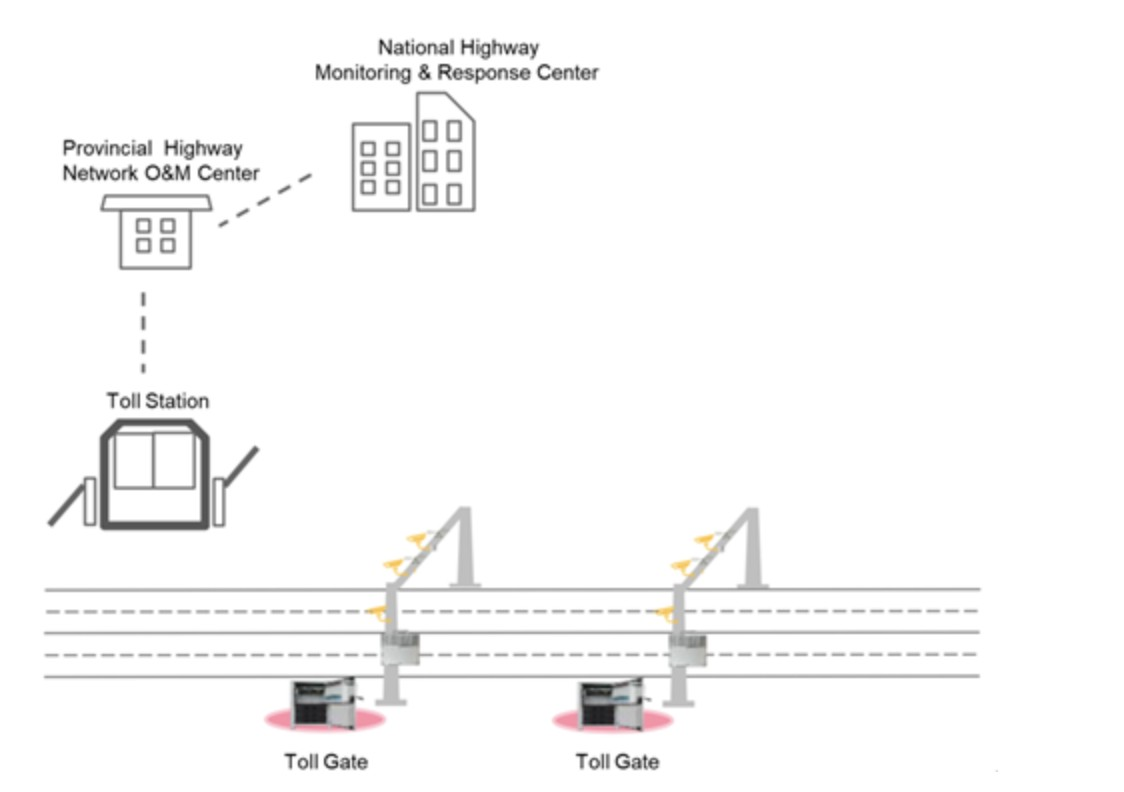
\includegraphics[width=0.8\textwidth]{resources/chapter-2/china-highways.jpg}
%   \caption{Implementasi Sistem \textit{ETC} di China \parencite{penelitianterkait1}}
%   \label{fig:china-highways}
% \end{figure}

% \begin{figure}[ht]
%   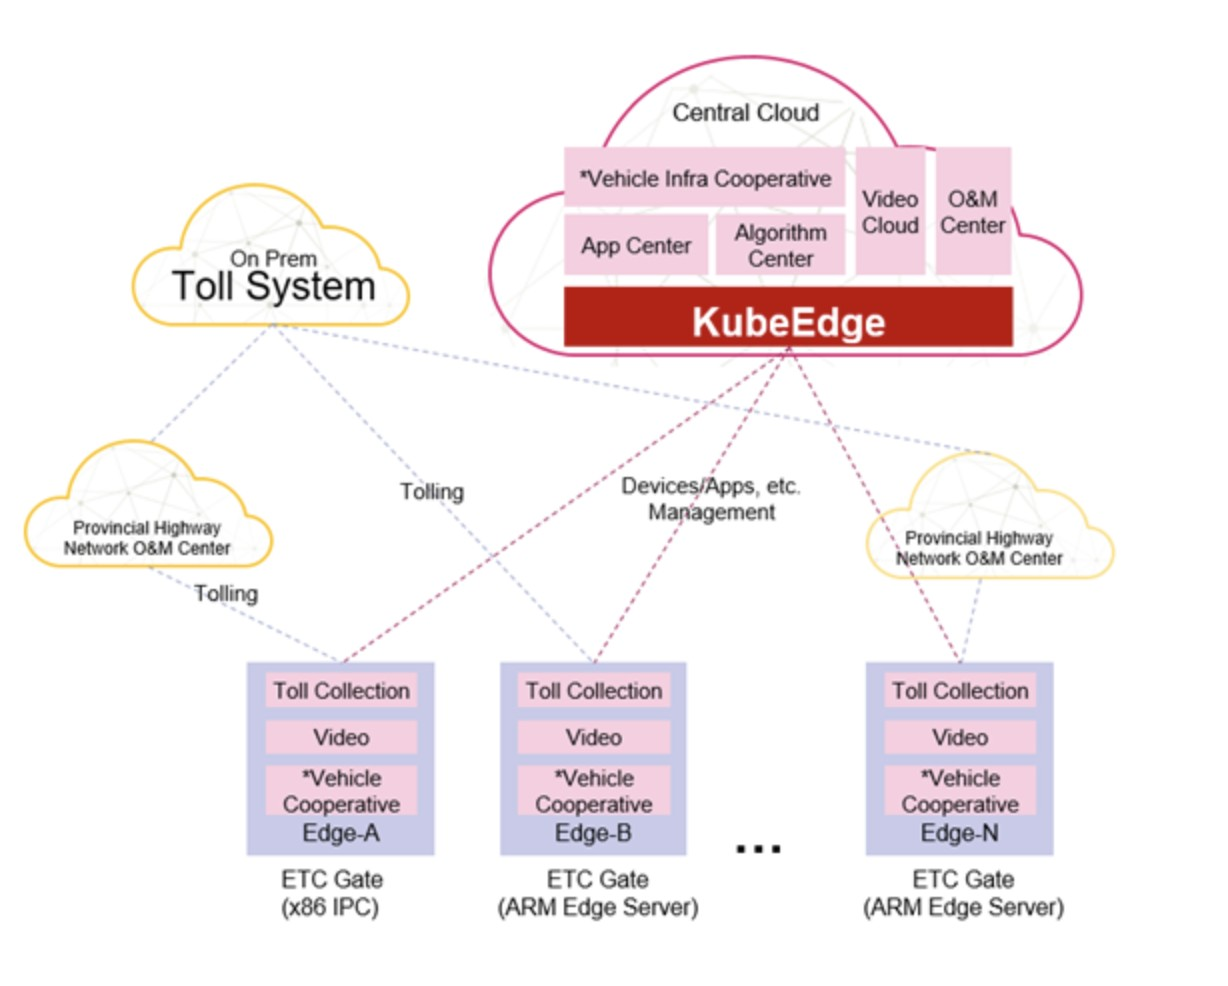
\includegraphics[width=0.8\textwidth]{resources/chapter-2/arsitektur-china-highways.jpg}
%   \caption{Arsitektur Sistem \textit{ETC} di China \parencite{penelitianterkait1}}
%   \label{fig:architecture-china-highways}
% \end{figure}

\chapter{Perbandingan Distribusi Kubernetes}

\bgroup
\begin{table}[ht]
  \def\arraystretch{1.5}
  \caption{Perbandingan Tiga Distribusi Kubenernetes pada Lingkungan IoT}
  \label{tab:perbandingan-distribusi-kubernetes}
  \centering
  \begin{tabular}{|p{1.7cm}|p{1.7cm}|p{2.3cm}|p{2cm}|p{1.5cm}|p{2cm}|}
    \hline
    \centering{Nama} & \centering{Dukungan arsitektur} & \centering{Instalasi dan Penggunaan}                                                                                                                           & \centering{Komputasi \textit{resource}}                  & Ukuran Cluster                                      & Fitur                            \\
    \hline
    K8s              & aarch64, armv7l, x86-64, macOS  & Sangat mudah, dapat diinstal dengan satu line command, dokumentasi lengkap                                                                                     & Penggunaan \textit{resource} yang minimal                & Kecil hingga menengah                               & Tidak seluruh fitur k8s tersedia \\
    \hline
    Microk8s         & aarch64, x86-64, armv7l         & Instalasi cukup sulit untuk dilakukan, kustomisasi cukup sulit untuk dilakukan, dokumentasi cukup sulit untuk dimeengerti                                      & Memerlukan \textit{resource} yang cukup besar            & Hanya untuk \textit{cluster} lokal                  & Tidak seluruh fitur k8s tersedia \\
    \hline
    KubeEdge         & aarch64, x86-64, armv7l         & Instalasi cukup kompleks serta perlu pemahaman yang lebih untuk menggunakannya. \textit{kustomisasi} yang cukup sulit, namun memiliki dokumentasi yang lengkap & Memerlukan sumber daya yang cukup besar dibandingkan K8s & Cocok untuk lingkungan distribusi serta skala besar & Lengkap                          \\
    \hline
  \end{tabular}
\end{table}
\egroup

\chapter{Tabel Kebutuhan}

\bgroup
\begin{table}[ht]
  \def\arraystretch{1.5}
  \caption{Kebutuhan Fungsional}
  \label{tab:kebutuhan-fungsional}
  \centering
  \begin{tabular}{|c|p{12cm}|}
    \hline
    ID  & Penjelasan                                                                                                      \\
    \hline
    F01 & Admin dapat melakukan registrasi perusahaan baru ke dalam sistem.                                               \\
    \hline
    F02 & Admin dapat melihat seluruh perushaan yang ada pada sistem.                                                     \\
    \hline
    F03 & Admin dapat menghapus perushaan yang ada pada sistem.                                                           \\
    \hline
    F04 & Admin dapat melakukan registrasi \textit{User} baru ke sebuah perusahaan pada sistem.
    \\
    \hline
    F05 & Admin dapat menghapus \textit{User} dari suatu perusahaan
    \\
    \hline
    F06 & \textit{User} dapat login ke dalam sistem.
    \\
    \hline
    F07 & \textit{User} dapat \textit{logout} dari sistem.

    \\
    \hline
    F08 & \textit{User} dapat melihat detail dari perushaan yang ada pada database sistem.                                \\
    \hline
    F09 & \textit{User} dapat melihat \textit{User} lain pada satu perusahaan yang sama                                   \\
    \hline
    F10 & \textit{User} dapat melakukan registrasi perangkat ke database sistem                                           \\
    \hline
    F11 & \textit{User} dapat melihat seluruh perangkat yang telah didaftarkan pada perushaannya                          \\
    \hline
    F12 & \textit{User} dapat menghapus perangkat yang telah didaftarkan di database                                      \\
    \hline
    F13 & \textit{User} dapat membuat \textit{groups} untuk mengelompokan beberapa perangkat                              \\
    \hline
    F14 & \textit{User} dapat melihat seluruh \textit{groups} yang telah terdaftar pada perusahannya                      \\
    \hline
    F15 & \textit{User} dapat menghapus \textit{groups} yang telah terdaftar pada perusahannya                            \\
    \hline
    F16 & \textit{User} dapat melihat hubungan antara perangkat dan \textit{groups} pada sistem dan begitupula sebaliknya \\
    \hline
    F17 & \textit{User} dapat membuat deployment images yang teraosiasi dengan perusahannya                               \\
    \hline
    F18 & \textit{User} dapat melihat deployment images yang teraosiasi dengan perusahannya                               \\
    \hline
  \end{tabular}
\end{table}
\egroup

\pagebreak

\bgroup
\begin{table}[ht]
  \def\arraystretch{1.7}
  \centering
  \begin{tabular}{|c|p{12cm}|}
    \hline
    ID  & Penjelasan                                                                                            \\

    \hline
    F19 & \textit{User} dapat menghapus deployment images yang teraosiasi dengan perusahannya                   \\
    \hline
    F20 & \textit{User} dapat membuat deployment plan yang teraosiasi dengan perushaannya                       \\
    \hline
    F21 & \textit{User} dapat melihat seluruh deployment plan yang terdaftar dan teraosiasi dengan perushaannya \\
    \hline
    F22 & \textit{User} dapat menghapus deployment plan yang terdaftar dan teraosiasi dengan perushaannya       \\
    \hline
    F23 & \textit{User} dapat melakukan deployment ke perangkat ataupun group dengan deployment plan pilihannya \\
    \hline
    F24 & \textit{User} dapat melihat riwayat dari deployment yang telah dilakukan ke perangkat ataupun group   \\
    \hline
  \end{tabular}
\end{table}
\egroup

\pagebreak

\bgroup
\begin{table}[ht]
  \def\arraystretch{1.7}
  \caption{Tabel Use case}
  \label{tab:penjelasan-usecase-diagram}
  \centering
  \begin{tabular}{|c|p{4cm}|p{7.5cm}|}
    \hline
    ID   & Use case                                   & Deskripsi                                                                                                                                  \\
    \hline
    UC01 & Mendaftarkan perusahaan                    & Sistem memberikan akses kepada admin untuk mendaftarkan perusahaan yang ingin mendaftar ke dalam sistem                                    \\
    \hline
    UC02 & Mendaftarkan \textit{user}                 & Sistem memberikan akses kepada admin untuk mendaftarkan \textit{user} ke perusahaan tertentu                                               \\
    \hline
    UC03 & Manajemen perusahaan                       & Sistem memberikan akses kepada admin untuk melakukan manajemen terhadap seluruh perusahaan yang terdaftar pada sistem                      \\
    \hline
    UC04 & Manajemen \textit{user}                    & Sistem memberikan akses kepada admin untuk melakukan manajemen terhadap seluruh \textit{user} yang terdaftar pada sistem                   \\
    \hline
    UC05 & Login                                      & Sistem memberikan akses kepada \textit{user}                                                                                               \\
    \hline
    UC06 & Melihat detail perusahaan                  & Sistem memberikan akses kepada \textit{user} untuk melihat perusahaanya                                                                    \\
    \hline
    UC07 & Melihat \textit{user} pada satu perusahaan & Sistem memberikan akses kepada \textit{user} user lainnya pada satu perusahaan                                                             \\

    \hline
    UC08 & Manajemen \textit{perangkat}               & Sistem memberikan akses kepada \textit{user} untuk melihat, membuat, serta menghapus \textit{perangkat} yang terdaftar pada sistem         \\
    \hline
    UC09 & Manajemen \textit{groups}                  & Sistem memberikan akses kepada \textit{user} untuk melihat, membuat, serta menghapus \textit{groups} yang terdaftar pada sistem            \\
    \hline
    UC10 & Manajemen \textit{deployment images}       & Sistem memberikan akses kepada \textit{user} untuk melihat, membuat, serta menghapus \textit{deployment images} yang terdaftar pada sistem \\
    \hline
    UC11 & Manajemen \textit{deployment plan}         & Sistem memberikan akses kepada \textit{user} untuk melihat, membuat, serta menghapus \textit{deployment plan} yang terdaftar pada sistem   \\
    \hline
    UC12 & Melakukan \textit{Remote deployment}       & Sistem memberikan akses kepada \textit{user} untuk melakukan \textit{deployment} kepada target perangakt ataupun \textit{groups}           \\
    \hline
    UC13 & Melihat riwayat \textit{deployment}        & Sistem memberikan akses kepada \textit{user} untuk melihat riwayat \textit{deployment} yang telah dilakukan                                \\
    \hline
  \end{tabular}
\end{table}
\egroup

\chapter{Tampilan halaman dashboard}
\label{appendix:tampilan-halaman-dashboard}

\begin{figure}[ht]
  \centering
  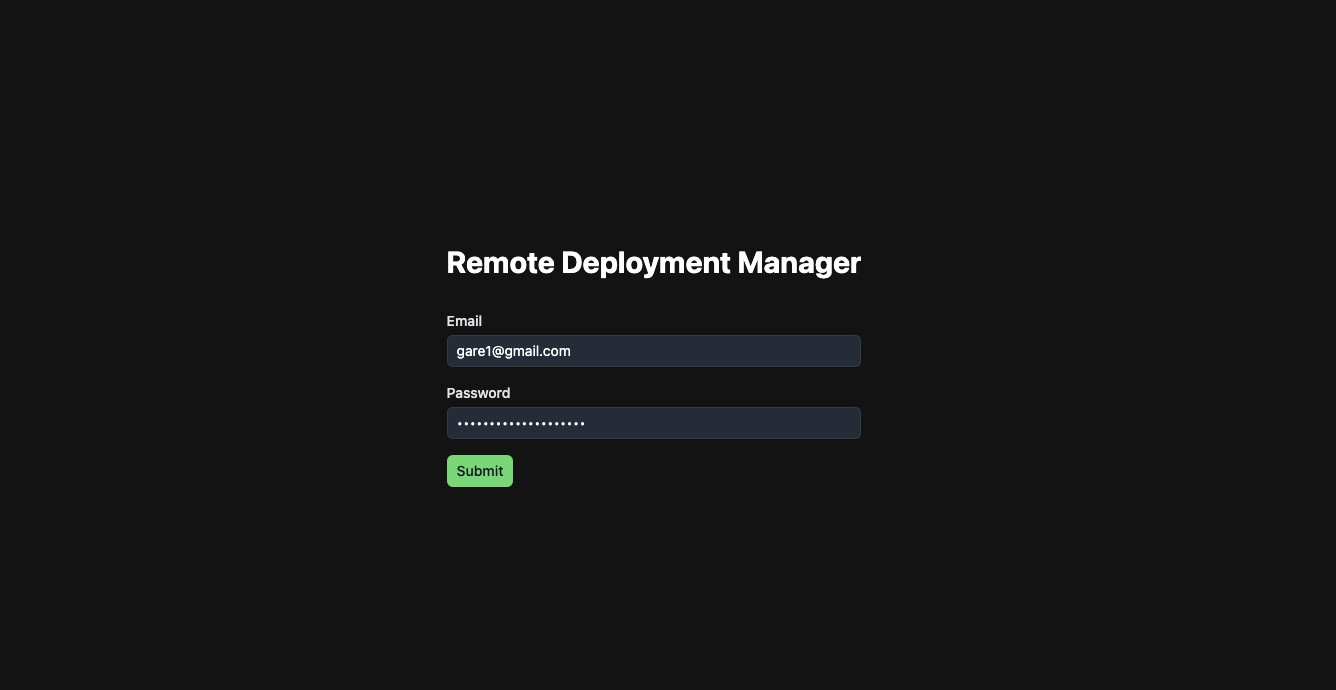
\includegraphics[width=1\textwidth]{resources/chapter-4/dashboard/login-page.jpg}
  \caption{Halaman Login}
  \label{fig:halaman-login}
\end{figure}

\begin{figure}[ht]
  \centering
  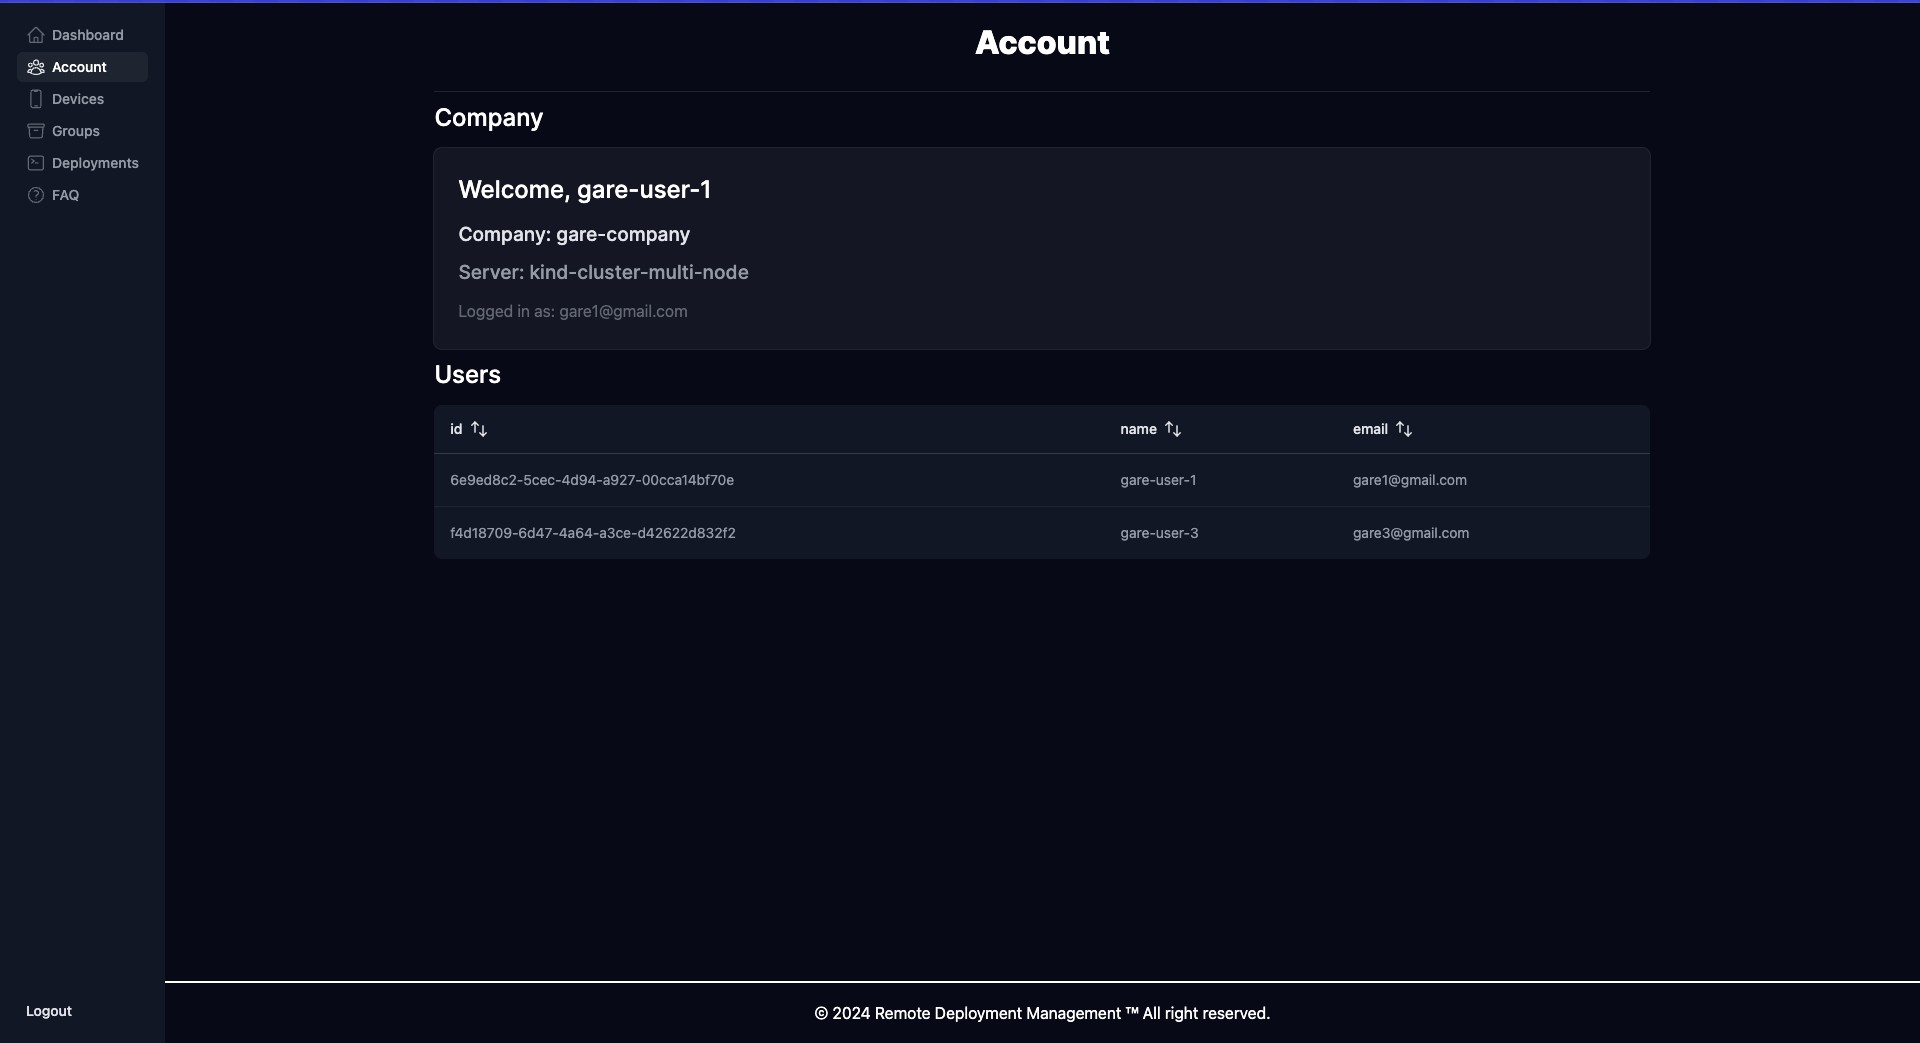
\includegraphics[width=1\textwidth]{resources/chapter-4/dashboard/account-page.jpg}
  \caption{Halaman \textit{Account}}
  \label{fig:halaman-account}
\end{figure}

\begin{figure}[ht]
  \centering
  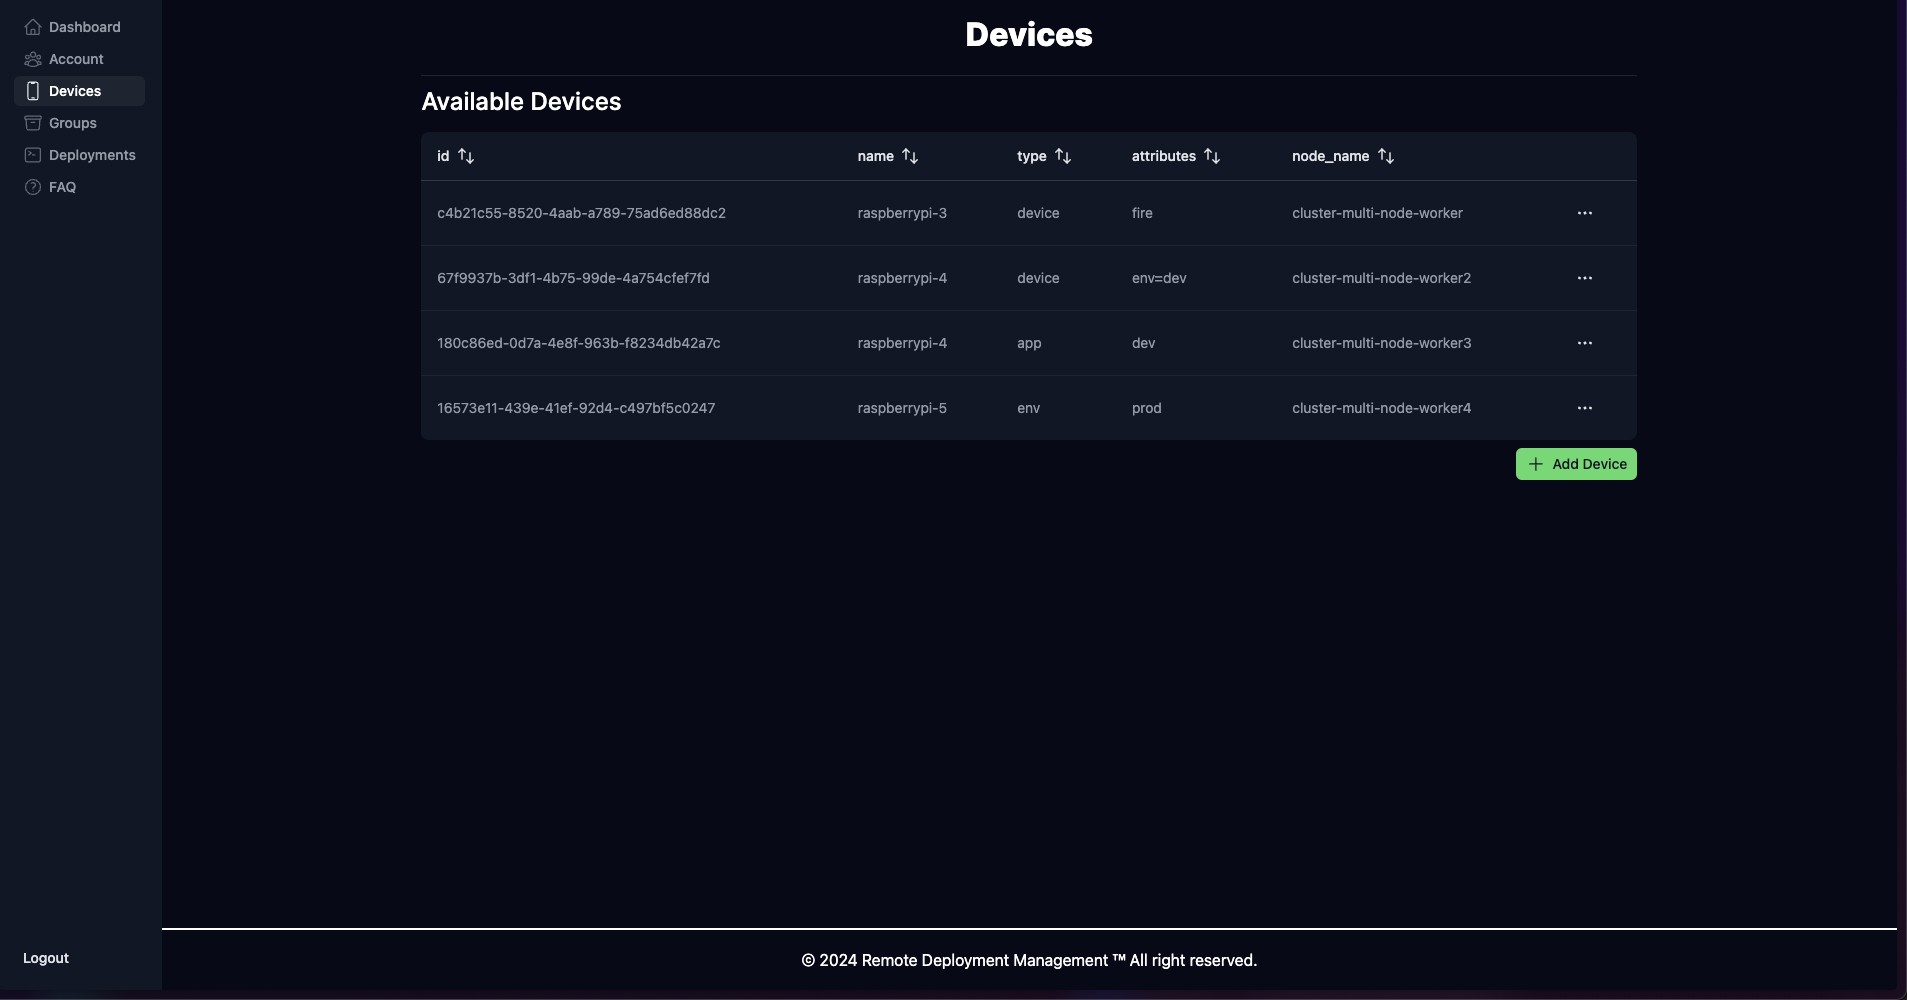
\includegraphics[width=1\textwidth]{resources/chapter-4/dashboard/device-page.jpg}
  \caption{Halaman \textit{Device}}
  \label{fig:halaman-device}
\end{figure}

\begin{figure}[ht]
  \centering
  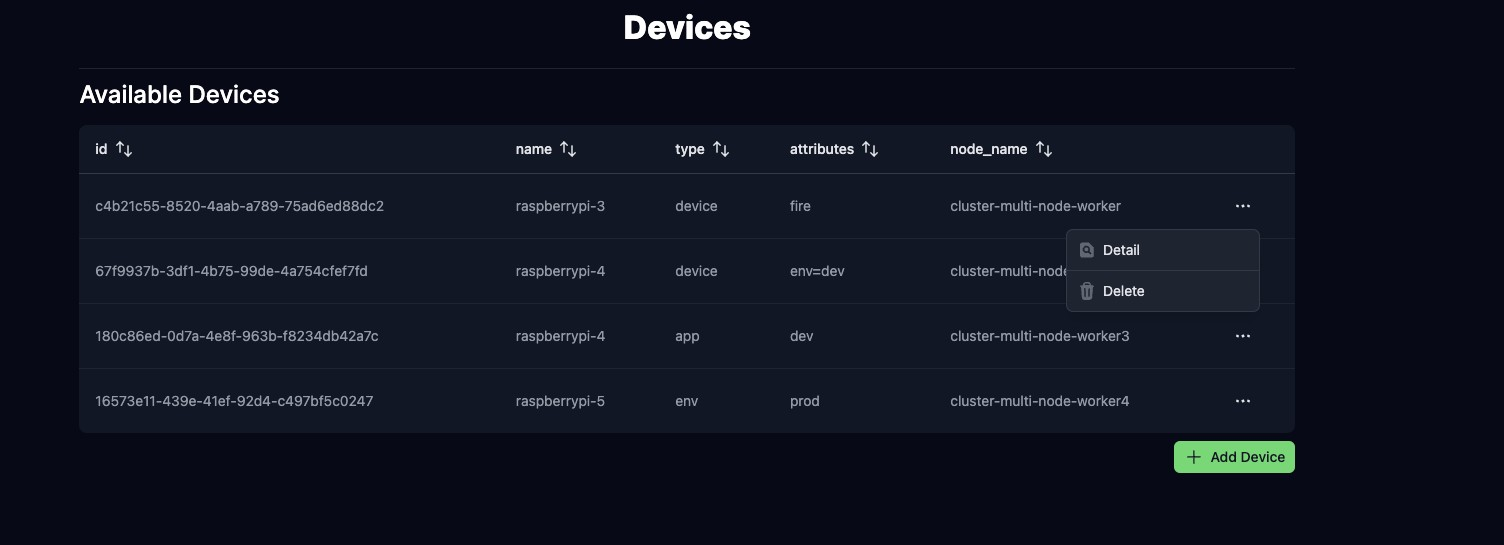
\includegraphics[width=1\textwidth]{resources/chapter-4/dashboard/device-page-actions.jpg}
  \caption{Actions pada Tabel \textit{Device}}
  \label{fig:halaman-device-actions}
\end{figure}

\begin{figure}[ht]
  \centering
  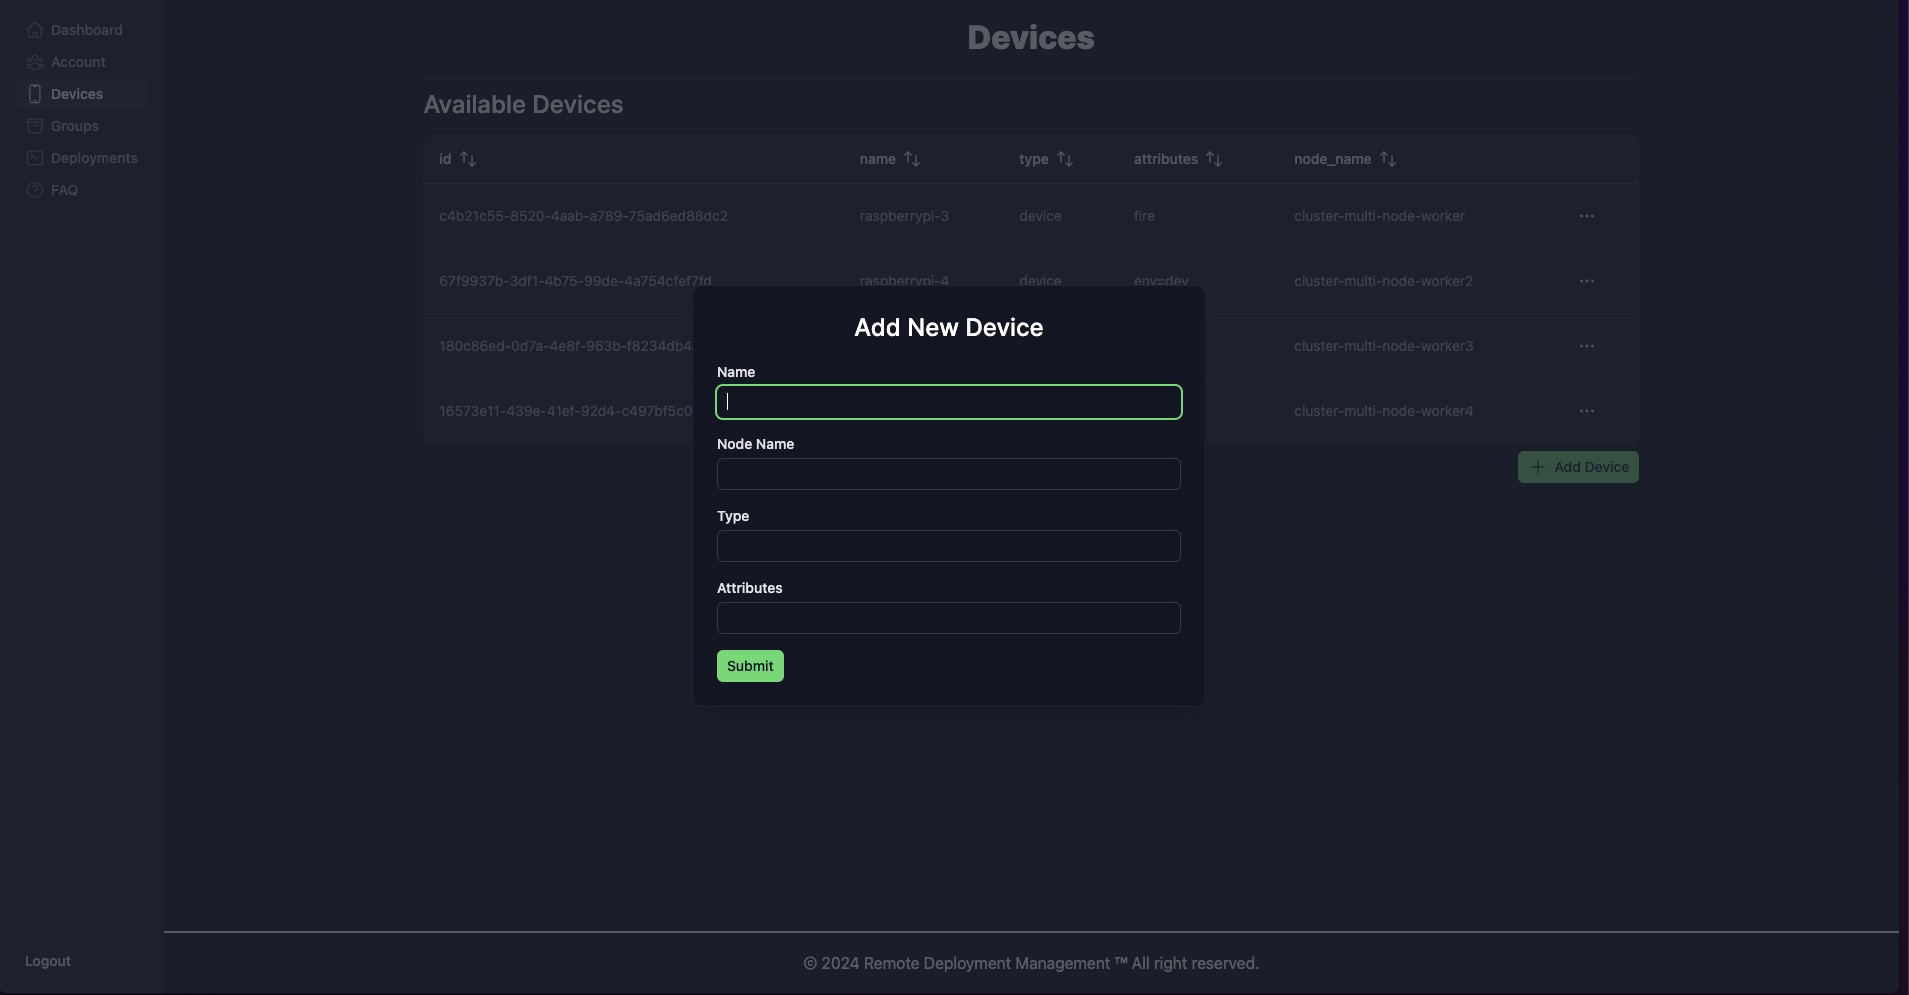
\includegraphics[width=1\textwidth]{resources/chapter-4/dashboard/device-page-add.jpg}
  \caption{Modal Menambahkan \textit{Device}}
  \label{fig:halaman-device-add}
\end{figure}

\begin{figure}[ht]
  \centering
  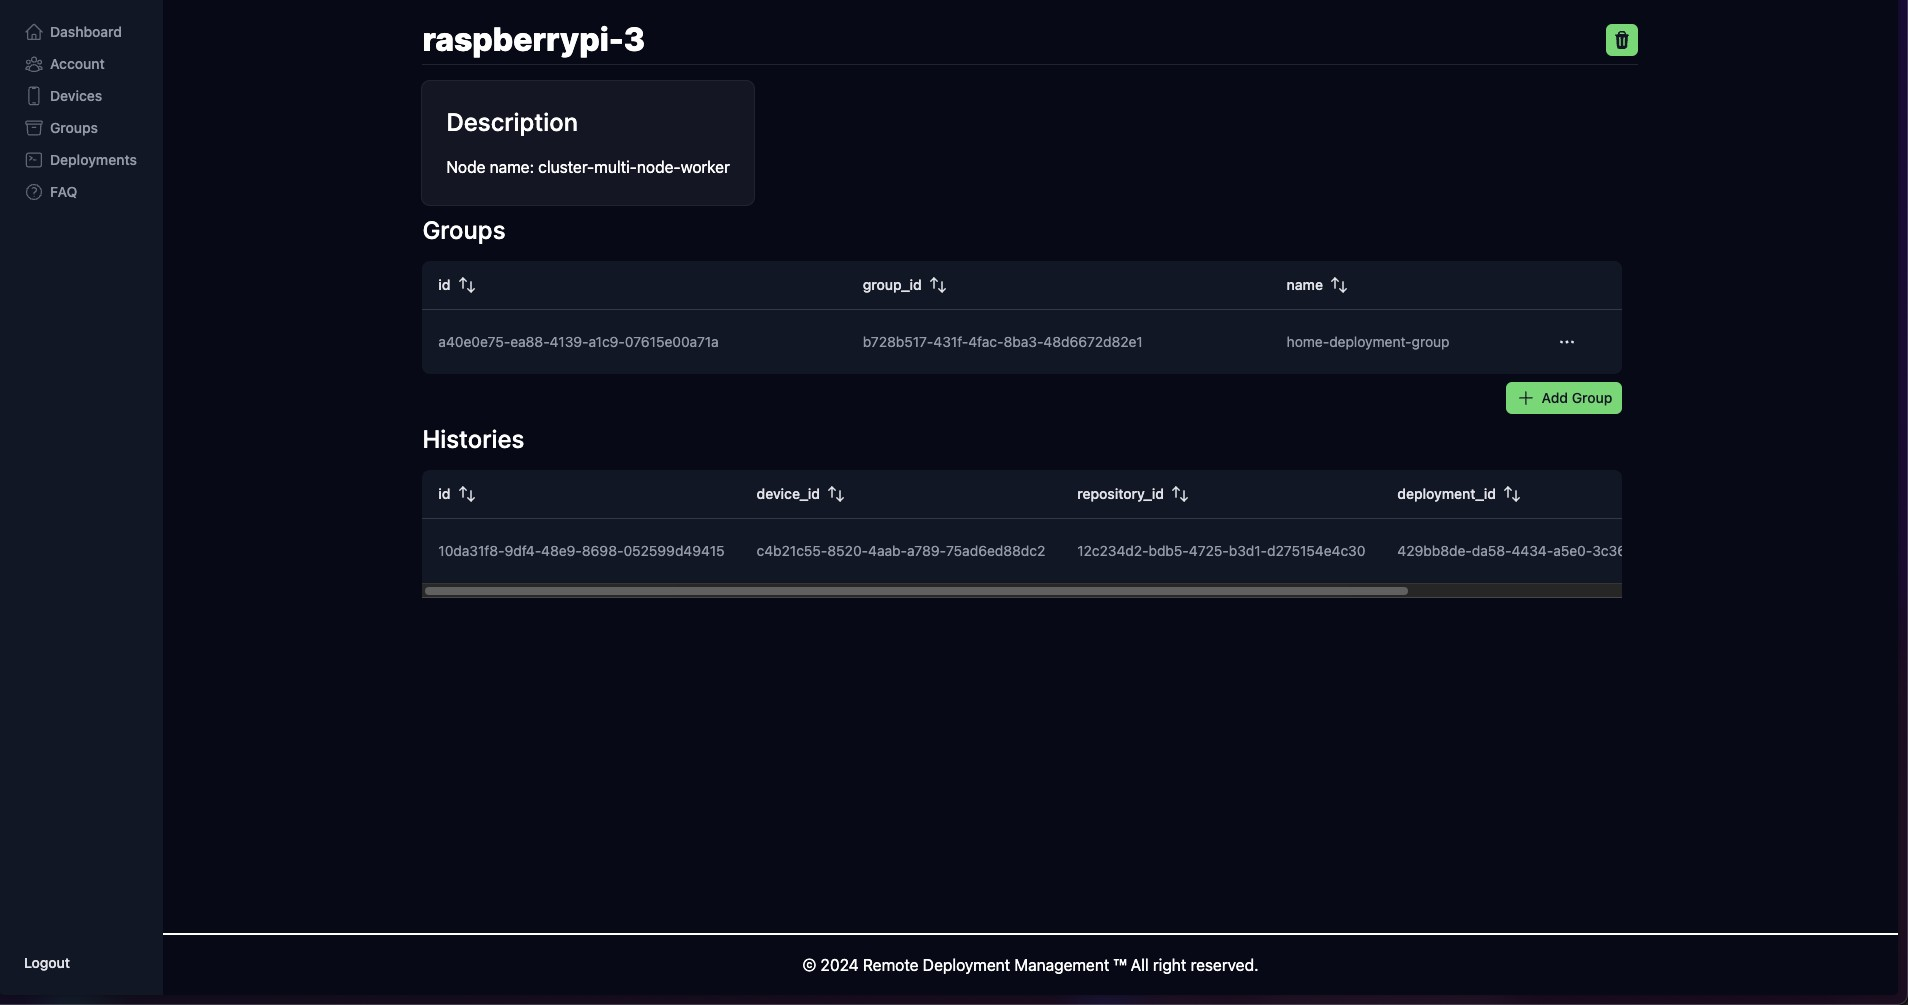
\includegraphics[width=1\textwidth]{resources/chapter-4/dashboard/device-detail-page.jpg}
  \caption{Halaman \textit{Device Detail}}
  \label{fig:halaman-device-detail}
\end{figure}

\begin{figure}[ht]
  \centering
  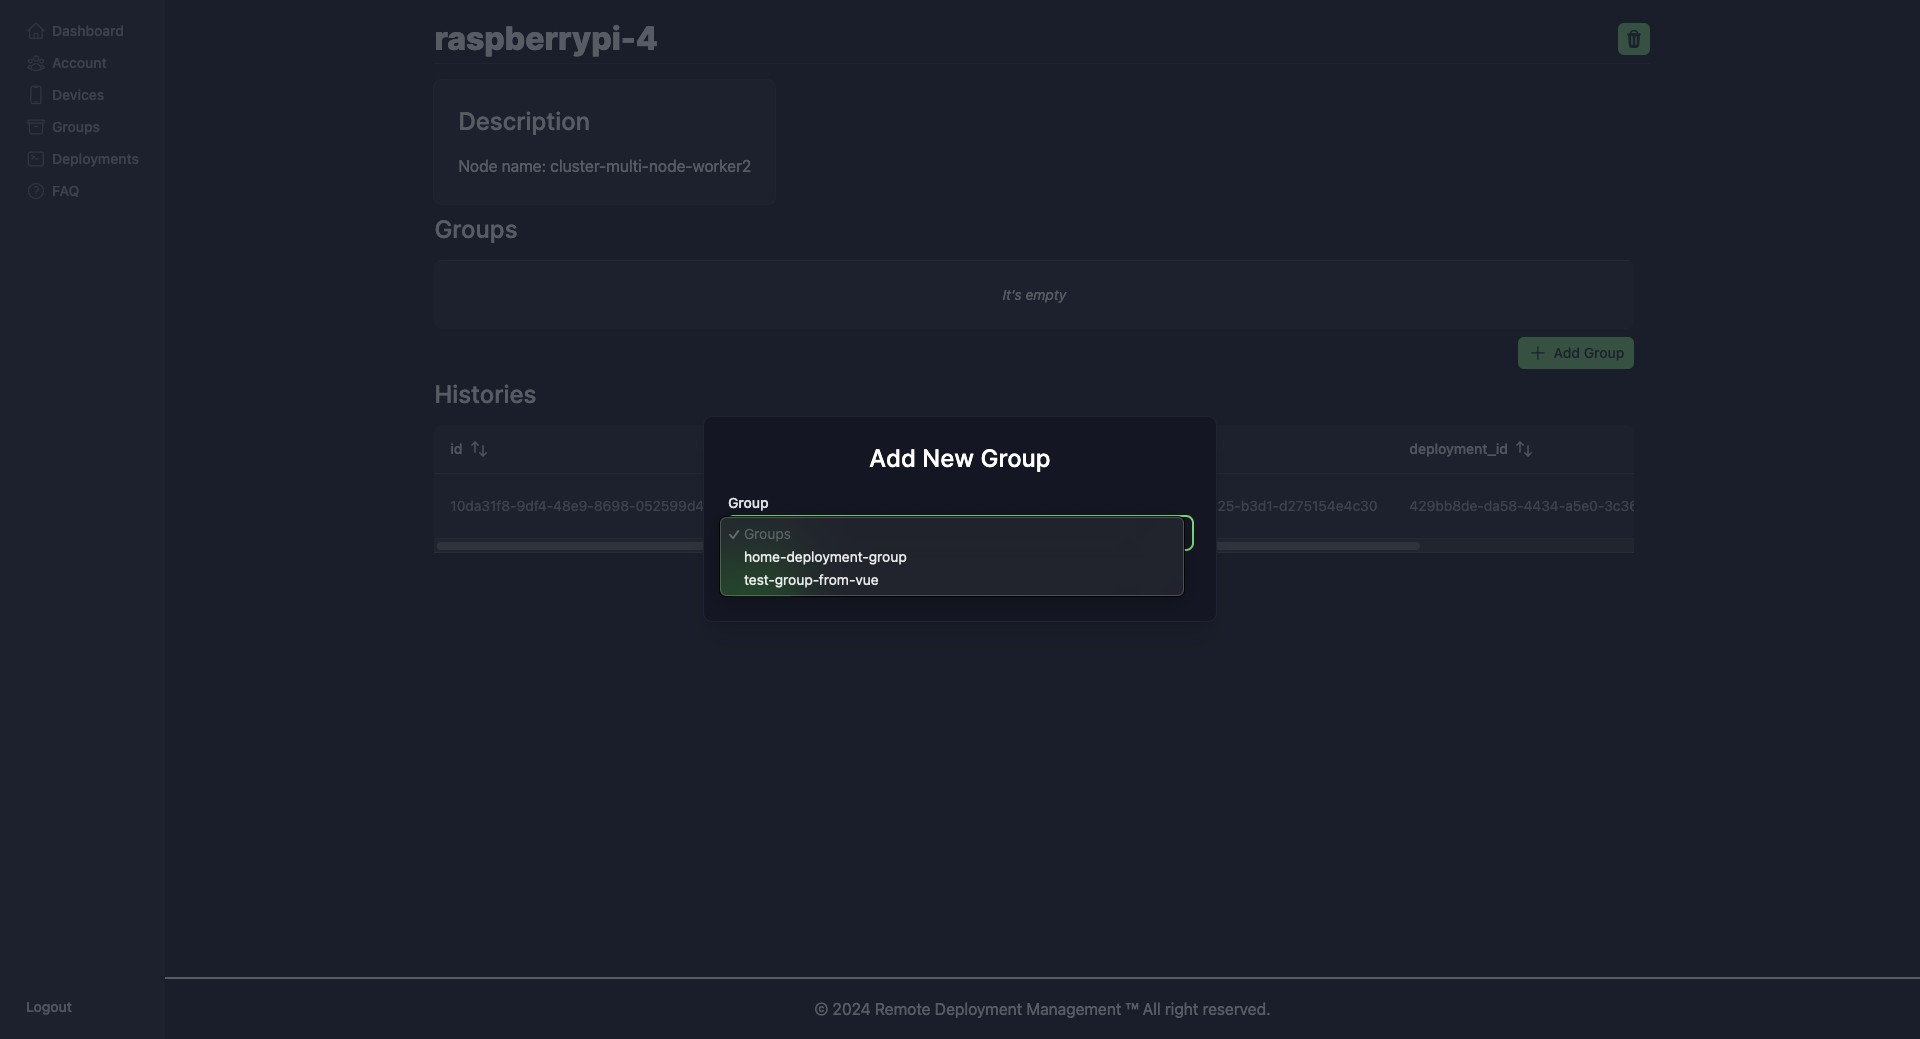
\includegraphics[width=1\textwidth]{resources/chapter-4/dashboard/device-detail-add-group.jpg}
  \caption{Modal Menambahkan \textit{Group} pada \textit{Device Detail}}
  \label{fig:halaman-device-detail-add-group}
\end{figure}

\begin{figure}[ht]
  \centering
  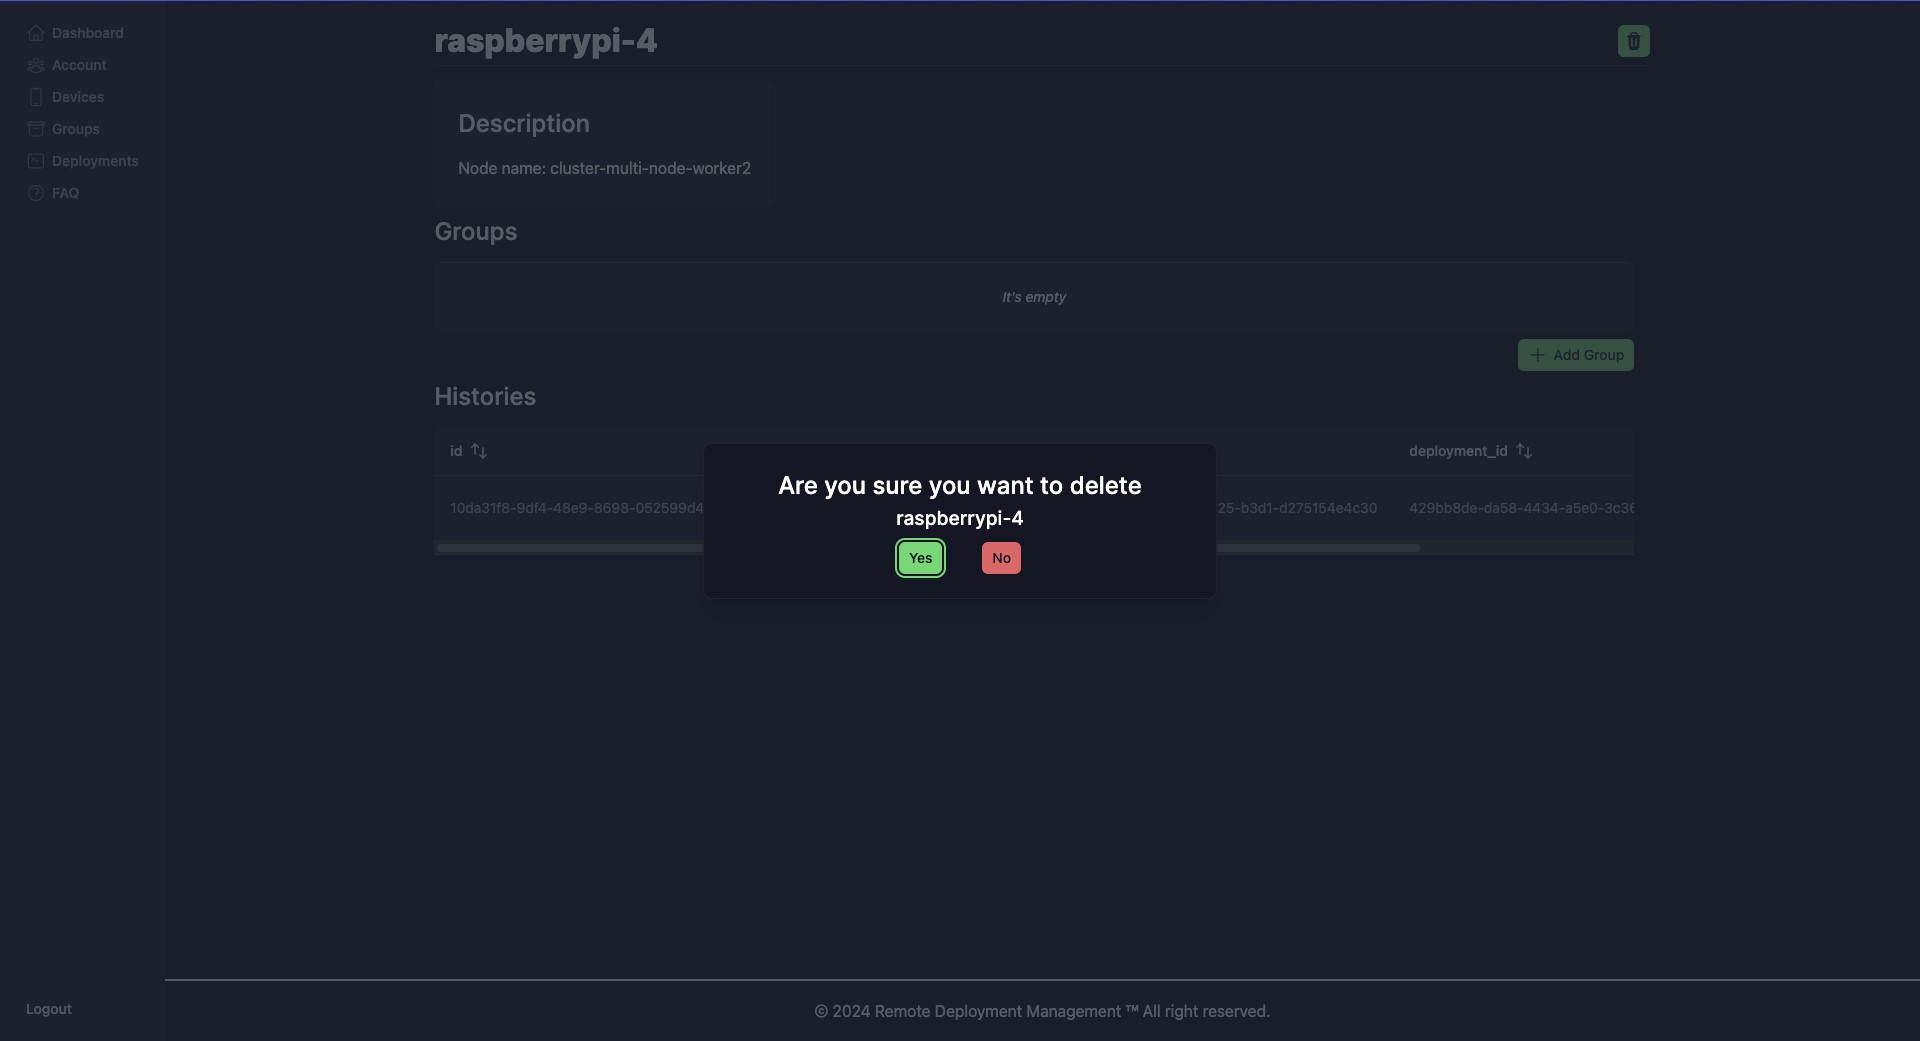
\includegraphics[width=1\textwidth]{resources/chapter-4/dashboard/device-detail-delete.jpg}
  \caption{Modal Menghapus Device pada Halaman \textit{Device Detail}}
  \label{fig:halaman-device-detail-delete}
\end{figure}

\begin{figure}[ht]
  \centering
  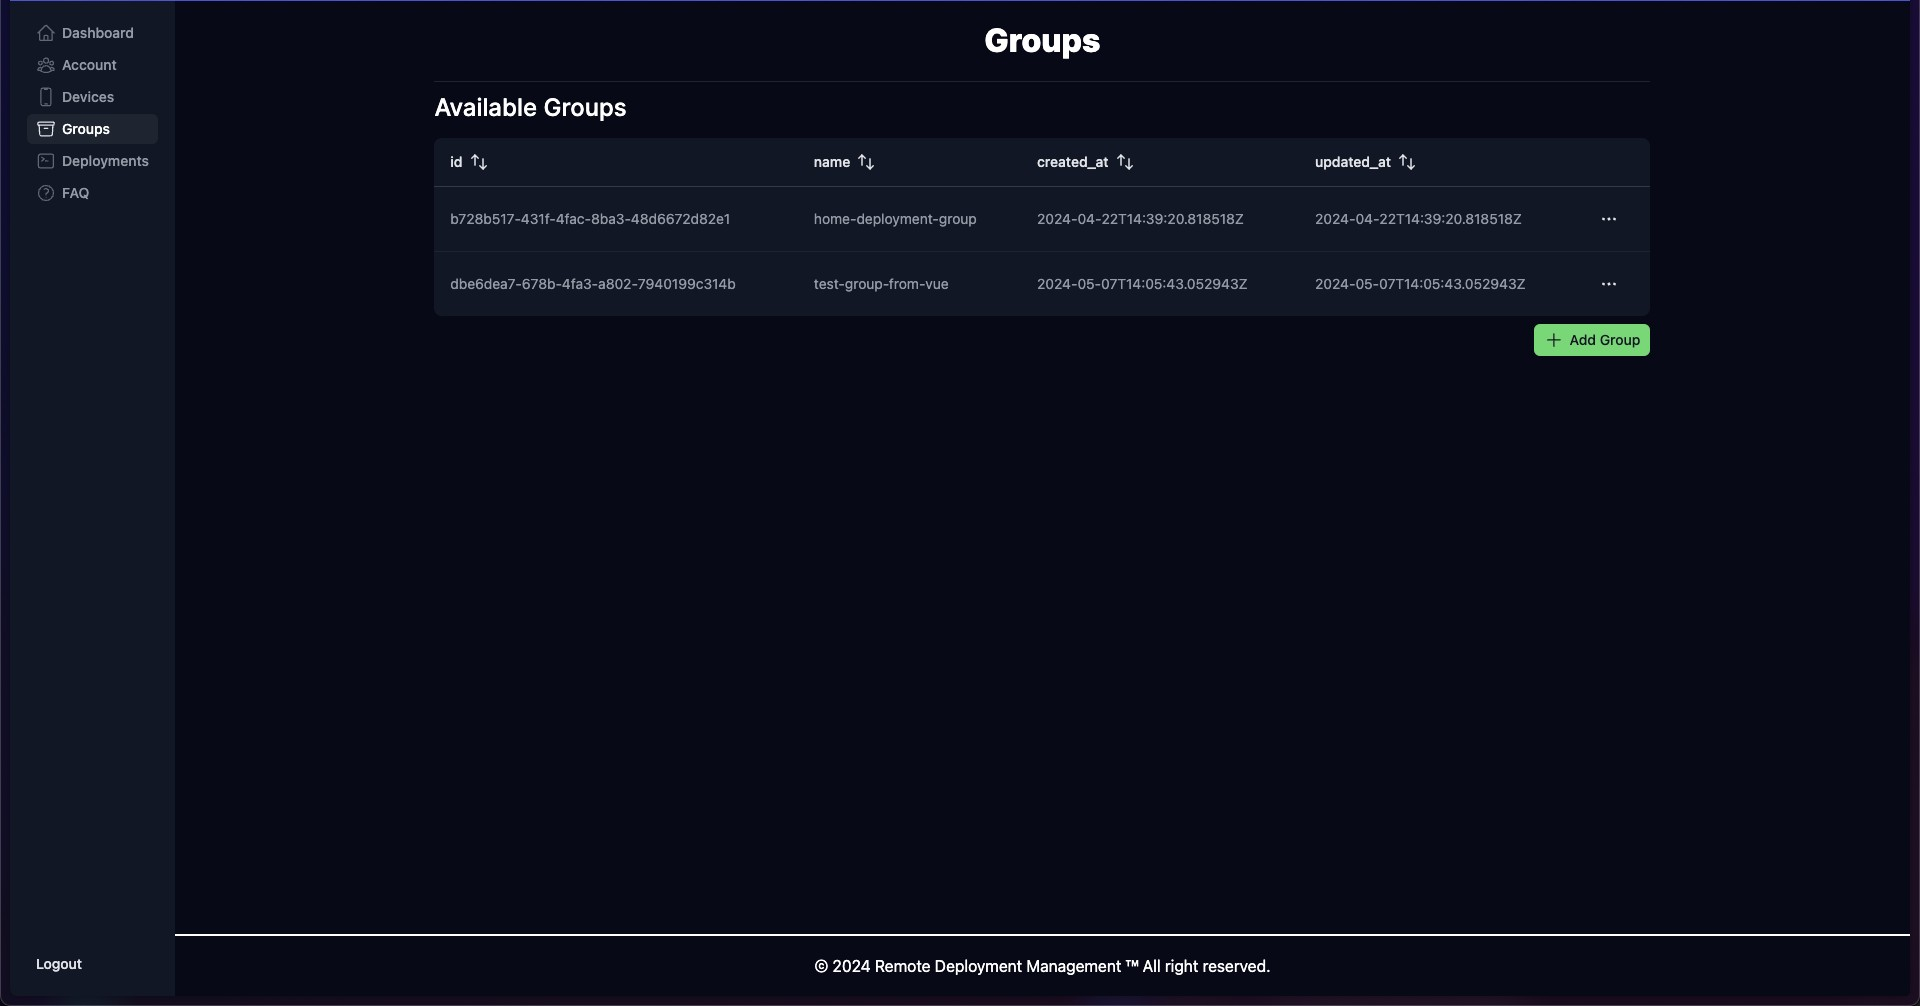
\includegraphics[width=1\textwidth]{resources/chapter-4/dashboard/groups-page.jpg}
  \caption{Halaman \textit{Groups}}
  \label{fig:halaman-groups}
\end{figure}

\begin{figure}[ht]
  \centering
  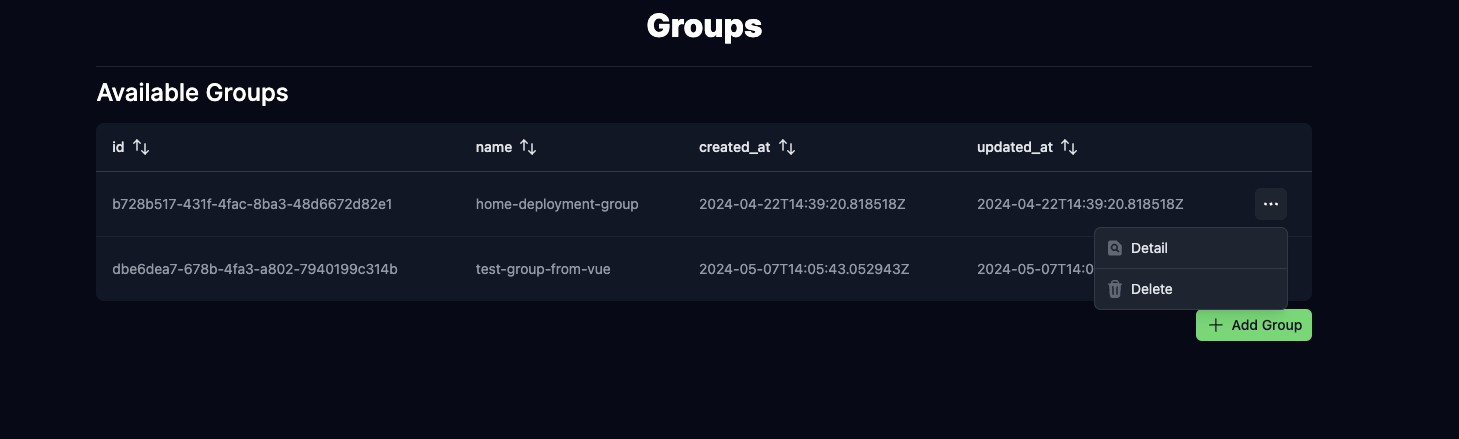
\includegraphics[width=1\textwidth]{resources/chapter-4/dashboard/groups-page-actions.jpg}
  \caption{\textit{Actions} pada Tabel \textit{Groups}}
  \label{fig:halaman-groups-actions}
\end{figure}

\begin{figure}[ht]
  \centering
  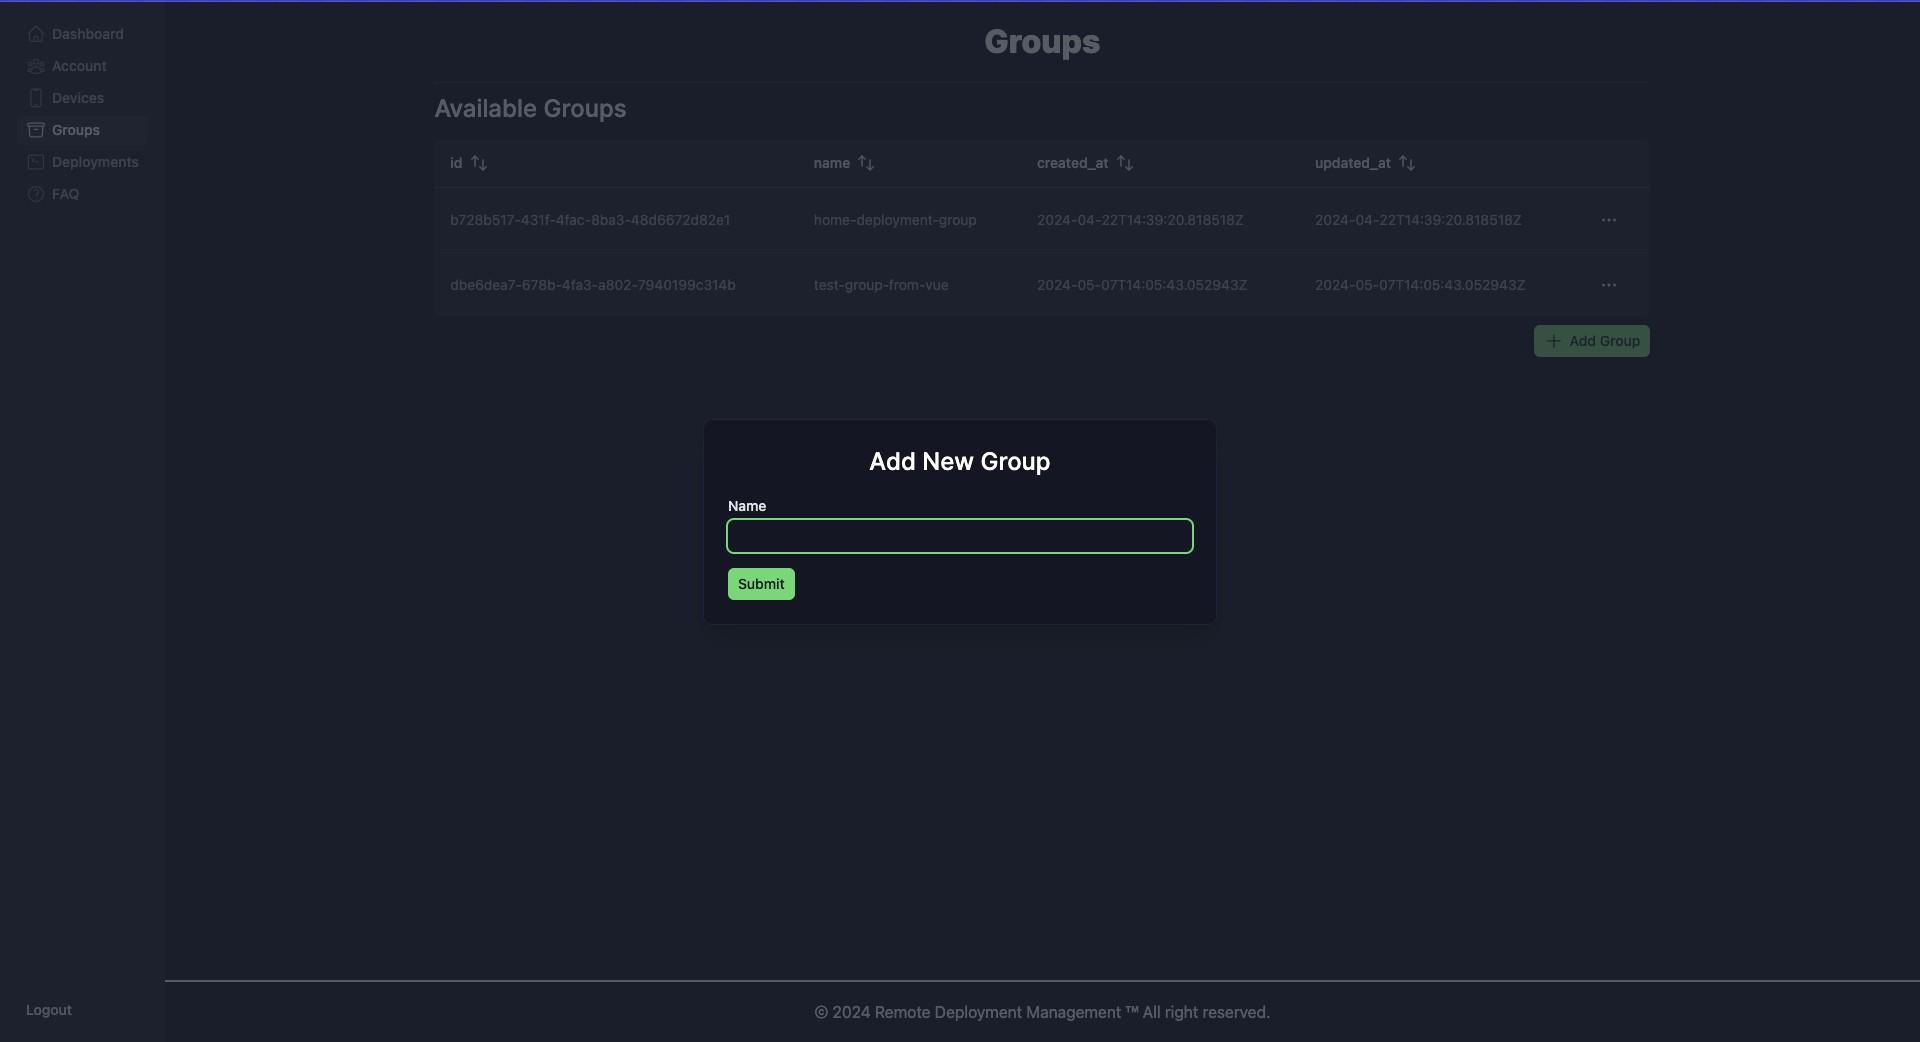
\includegraphics[width=1\textwidth]{resources/chapter-4/dashboard/groups-page-add.jpg}
  \caption{Modal Menambahkan \textit{groups}}
  \label{fig:halaman-groups-add}
\end{figure}

\begin{figure}[ht]
  \centering
  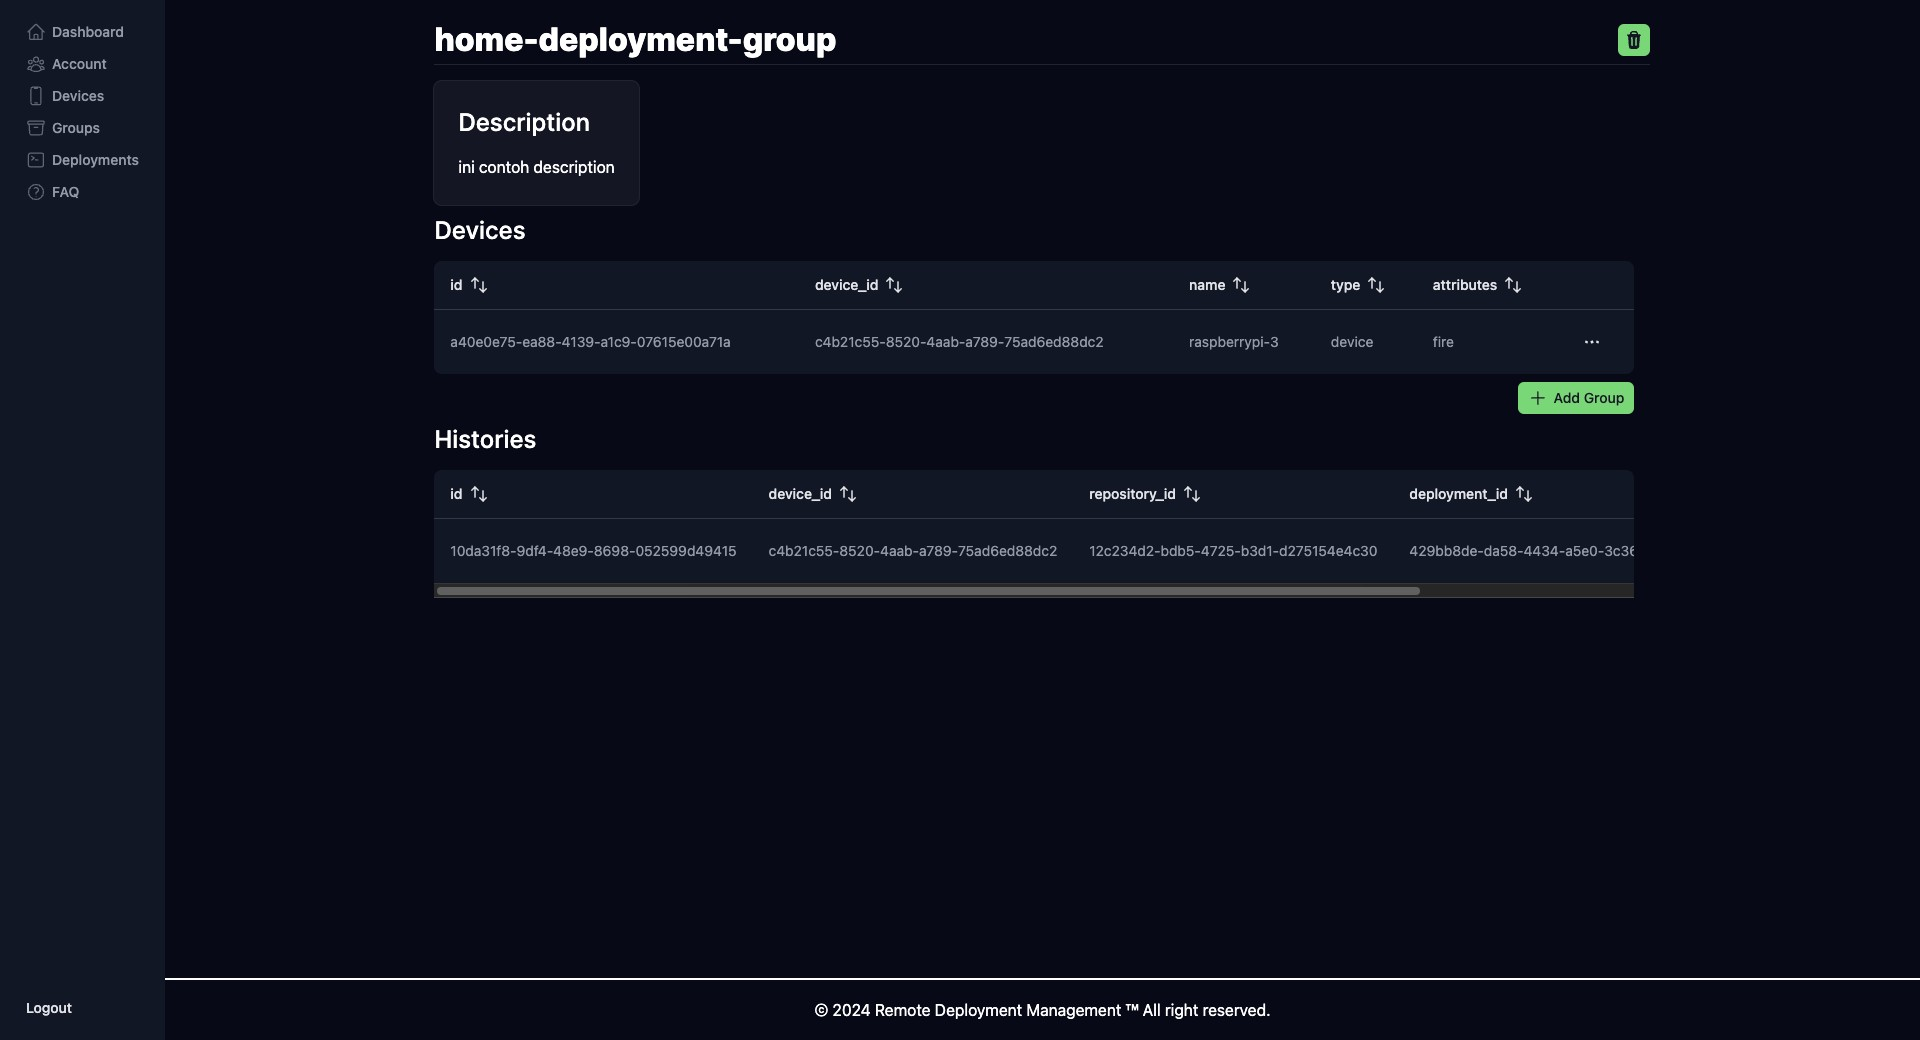
\includegraphics[width=1\textwidth]{resources/chapter-4/dashboard/groups-detail-page.jpg}
  \caption{Halaman \textit{groups detail}}
  \label{fig:halaman-groups-detail}
\end{figure}

\begin{figure}[ht]
  \centering
  \caption{Modal Menambahkan \textit{Group} pada \textit{Groups Detail}}
  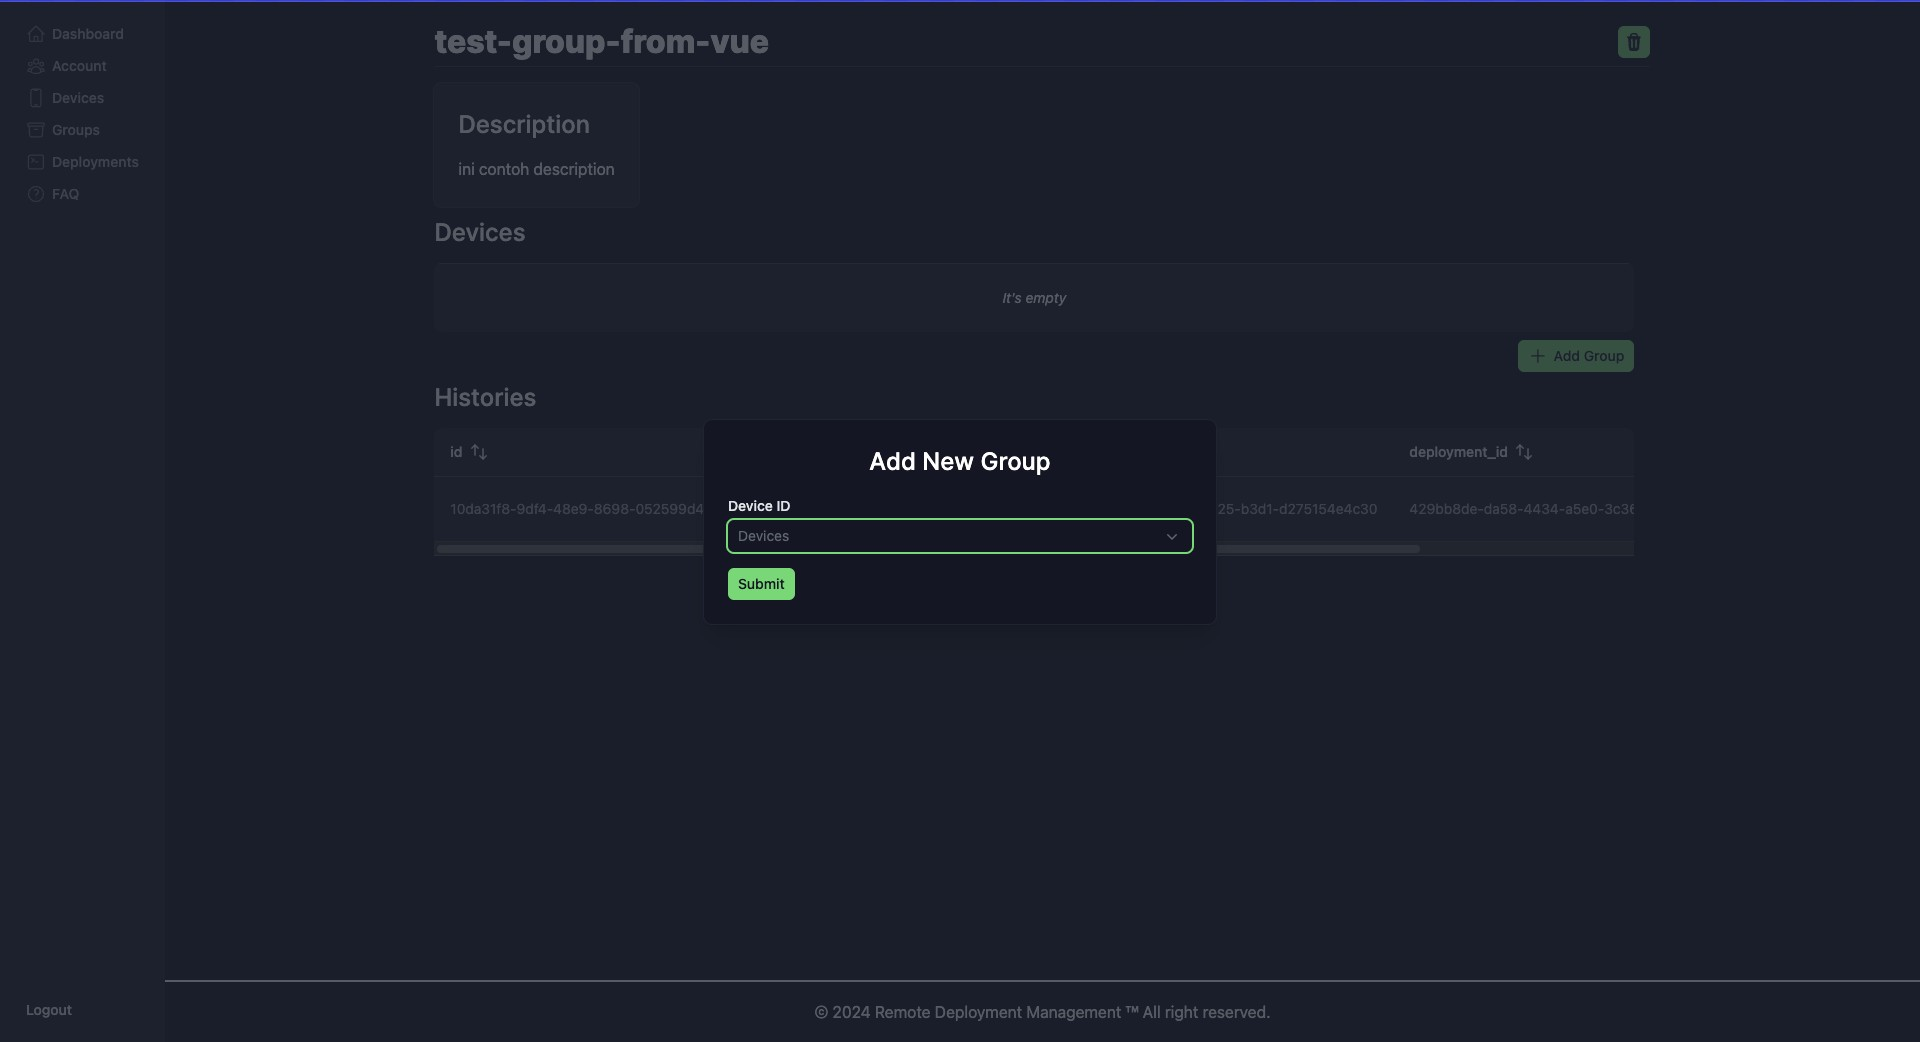
\includegraphics[width=1\textwidth]{resources/chapter-4/dashboard/groups-detail-add-device.jpg}
  \label{fig:halaman-groups-detail-add-group}
\end{figure}

\begin{figure}[ht]
  \centering
  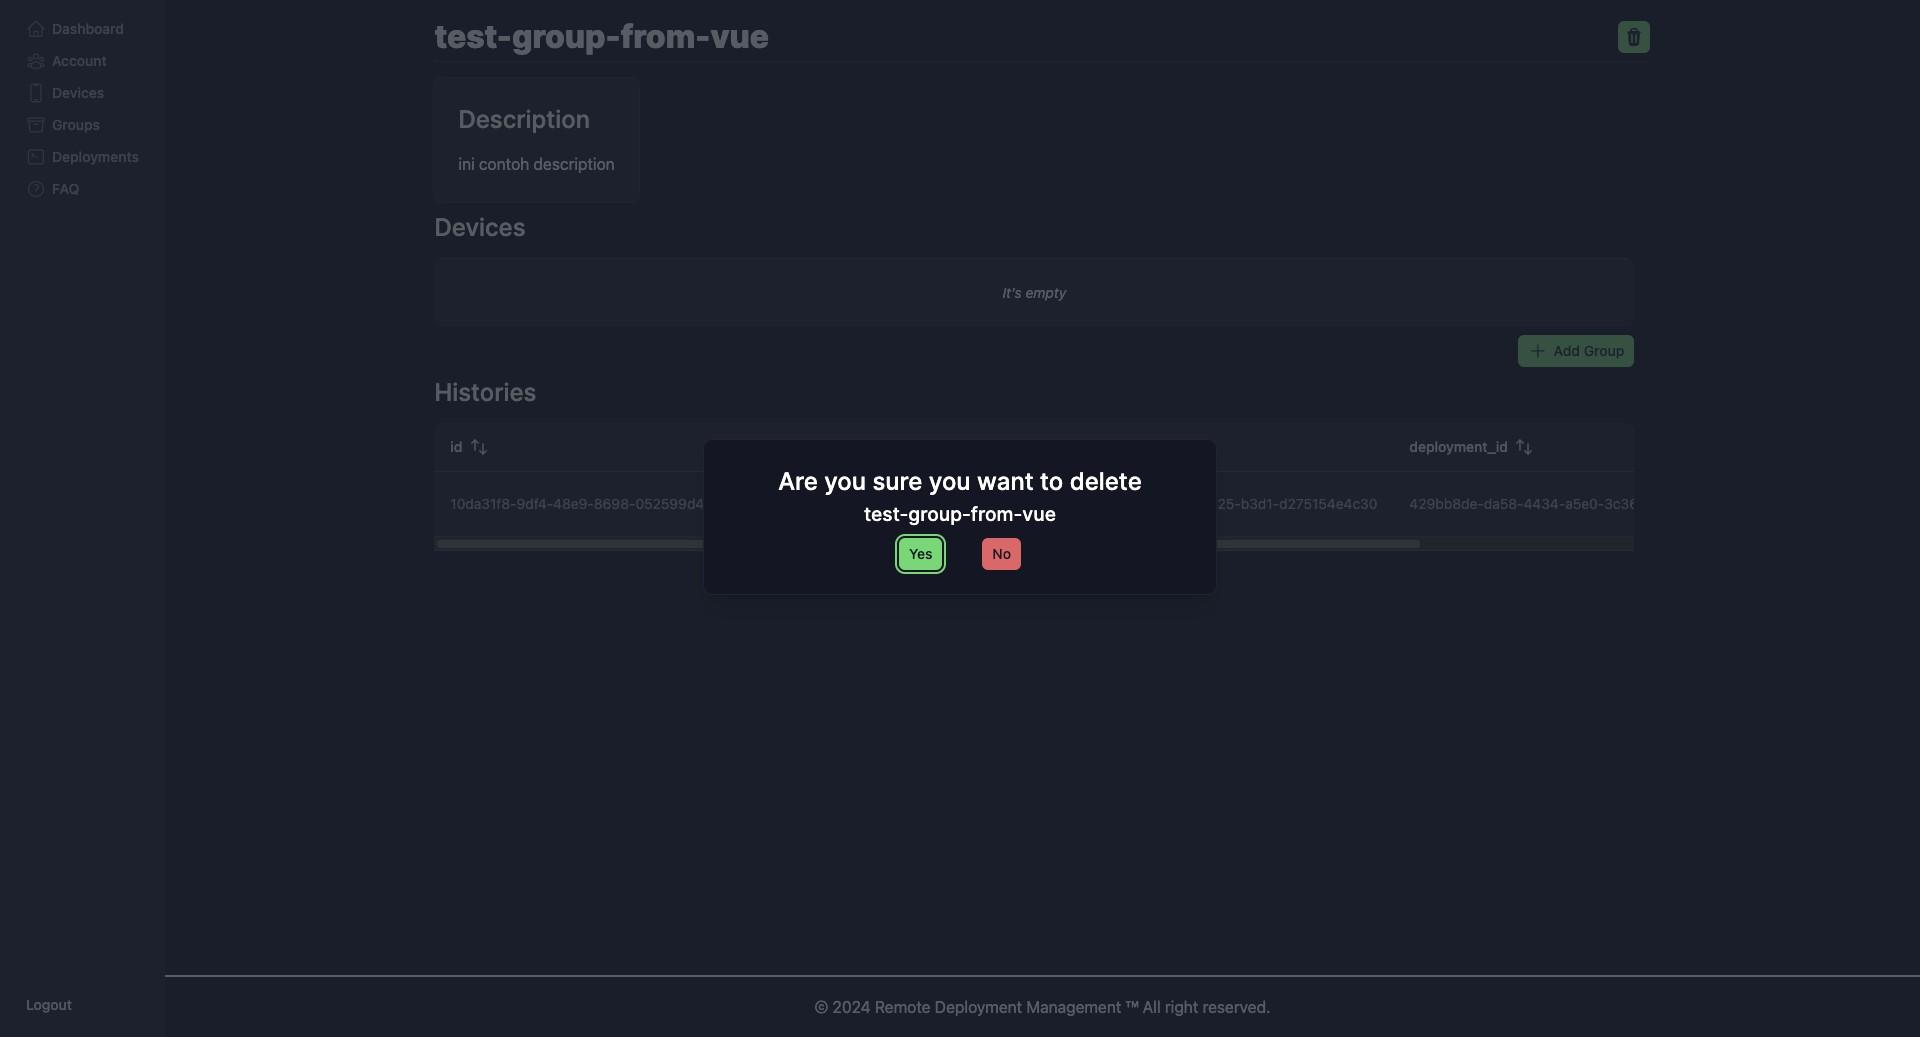
\includegraphics[width=1\textwidth]{resources/chapter-4/dashboard/groups-detail-delete.jpg}
  \caption{Modal Menghapus \textit{Groups} pada Halaman \textit{Groups Detail}}
  \label{fig:halaman-groups-detail-delete}
\end{figure}

\begin{figure}[ht]
  \centering
  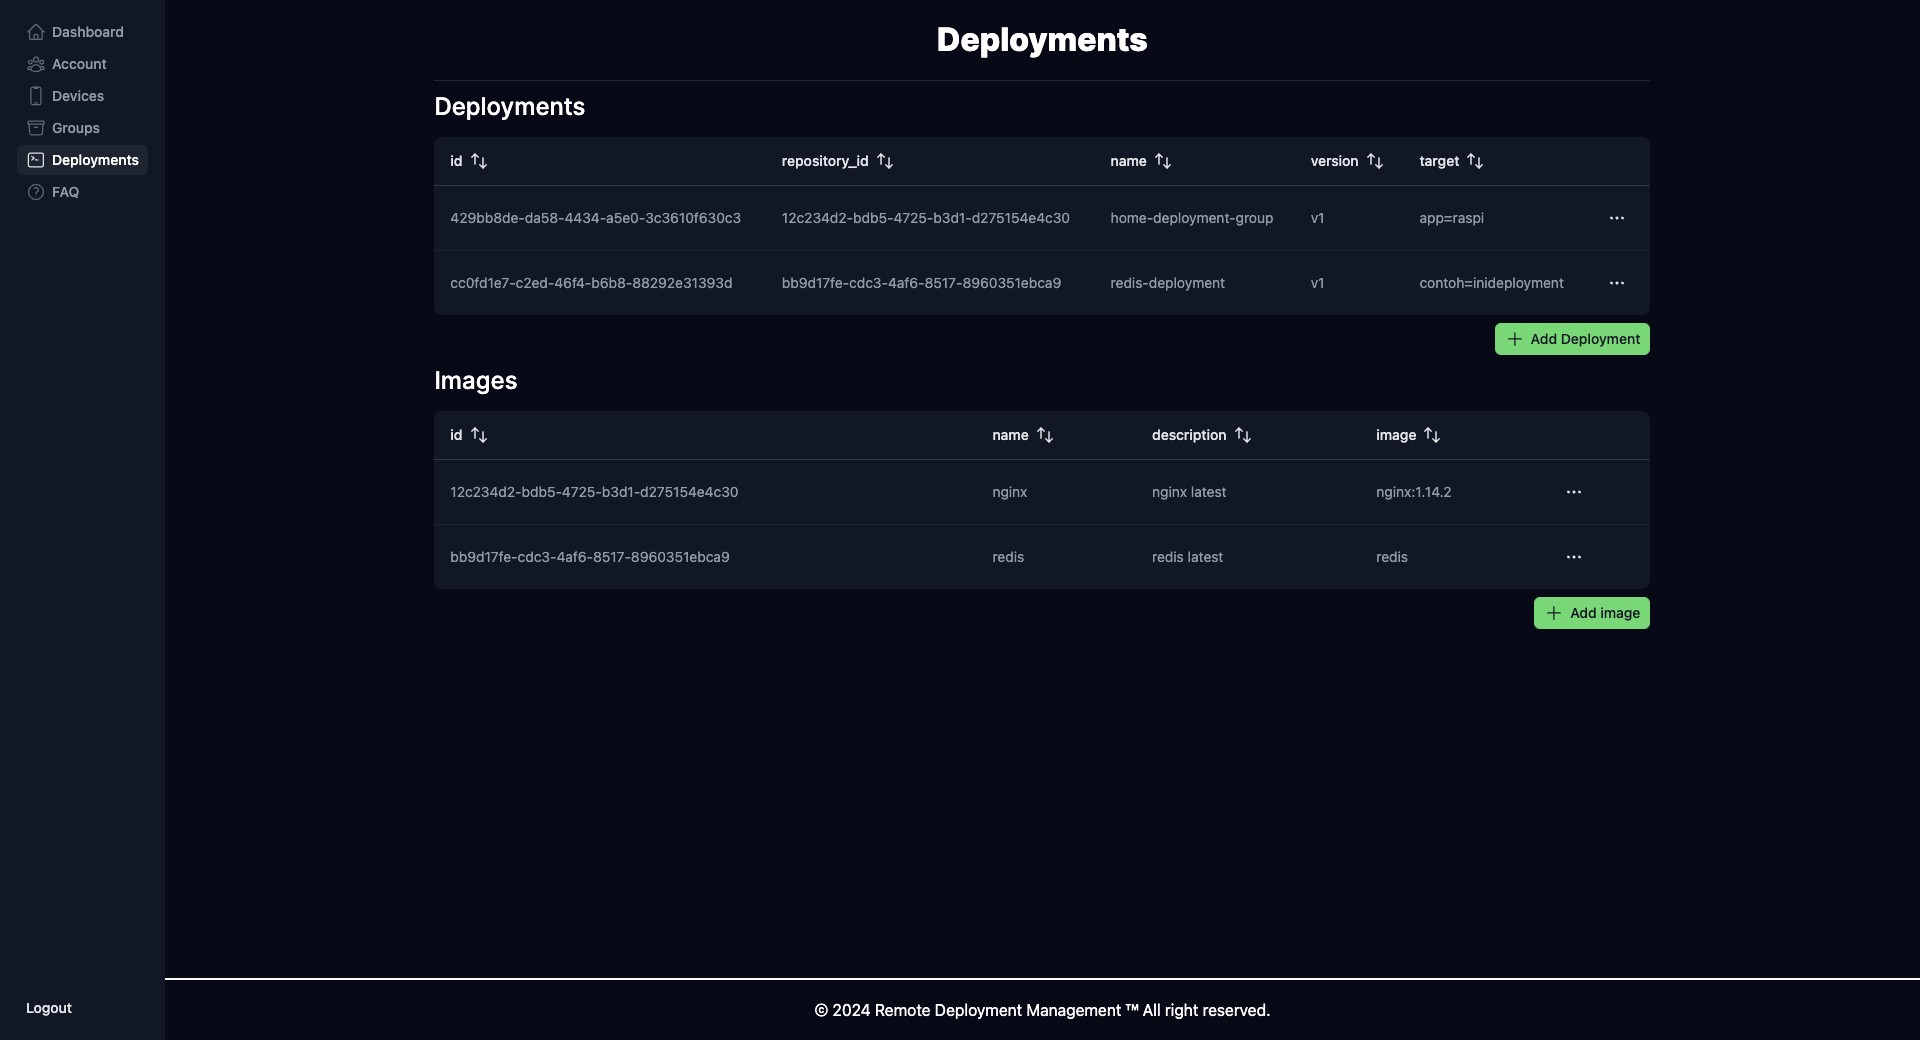
\includegraphics[width=1\textwidth]{resources/chapter-4/dashboard/deployment-page.jpg}
  \caption{Halaman \textit{Deployment}}
  \label{fig:halaman-deployment}
\end{figure}

\begin{figure}[ht]
  \centering
  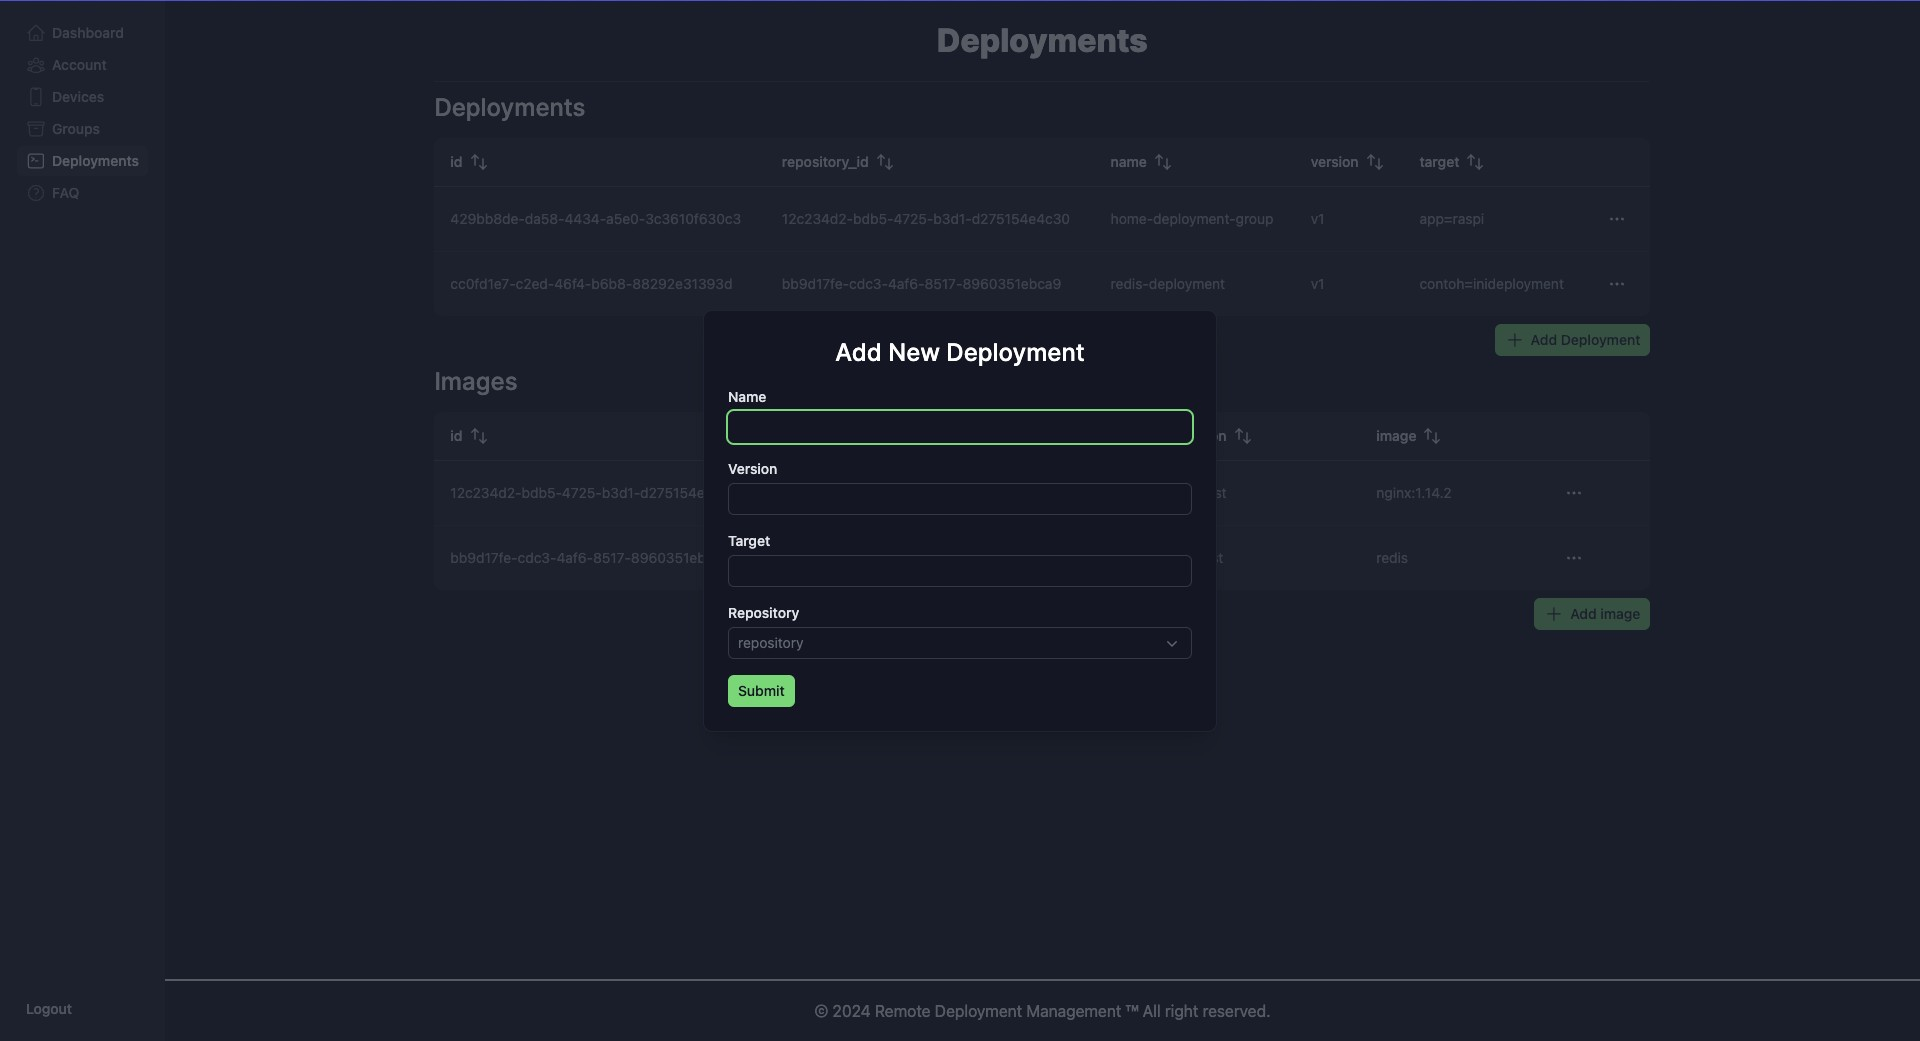
\includegraphics[width=1\textwidth]{resources/chapter-4/dashboard/deployment-page-add-deployment.jpg}
  \caption{Modal Menambahkan \textit{Deployment}}
  \label{fig:halaman-deployment-add-deployment}
\end{figure}

\begin{figure}[ht]
  \centering
  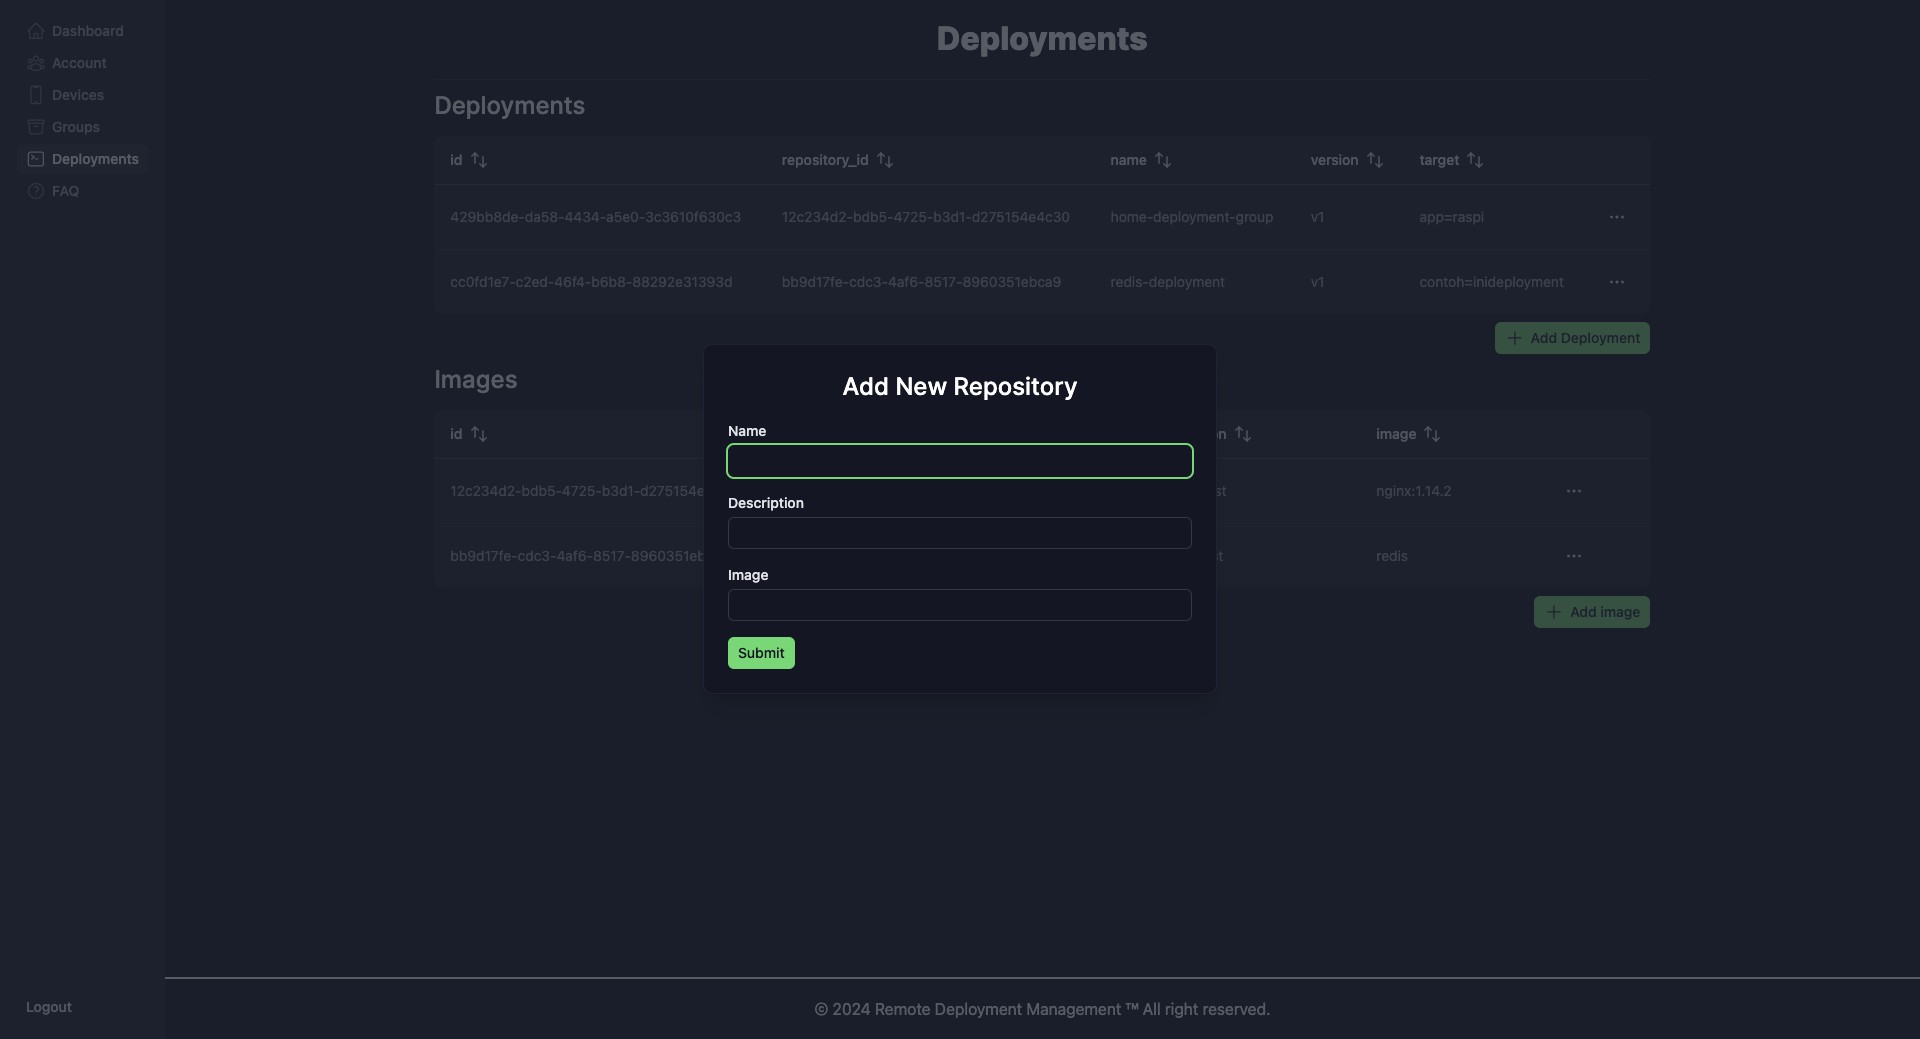
\includegraphics[width=1\textwidth]{resources/chapter-4/dashboard/deployment-page-add-repostory.jpg}
  \caption{Modal Menambahkan \textit{Image} Pada Halaman \textit{Deployment}}
  \label{fig:halaman-deployment-add-repostory}
\end{figure}

\begin{figure}[ht]
  \centering
  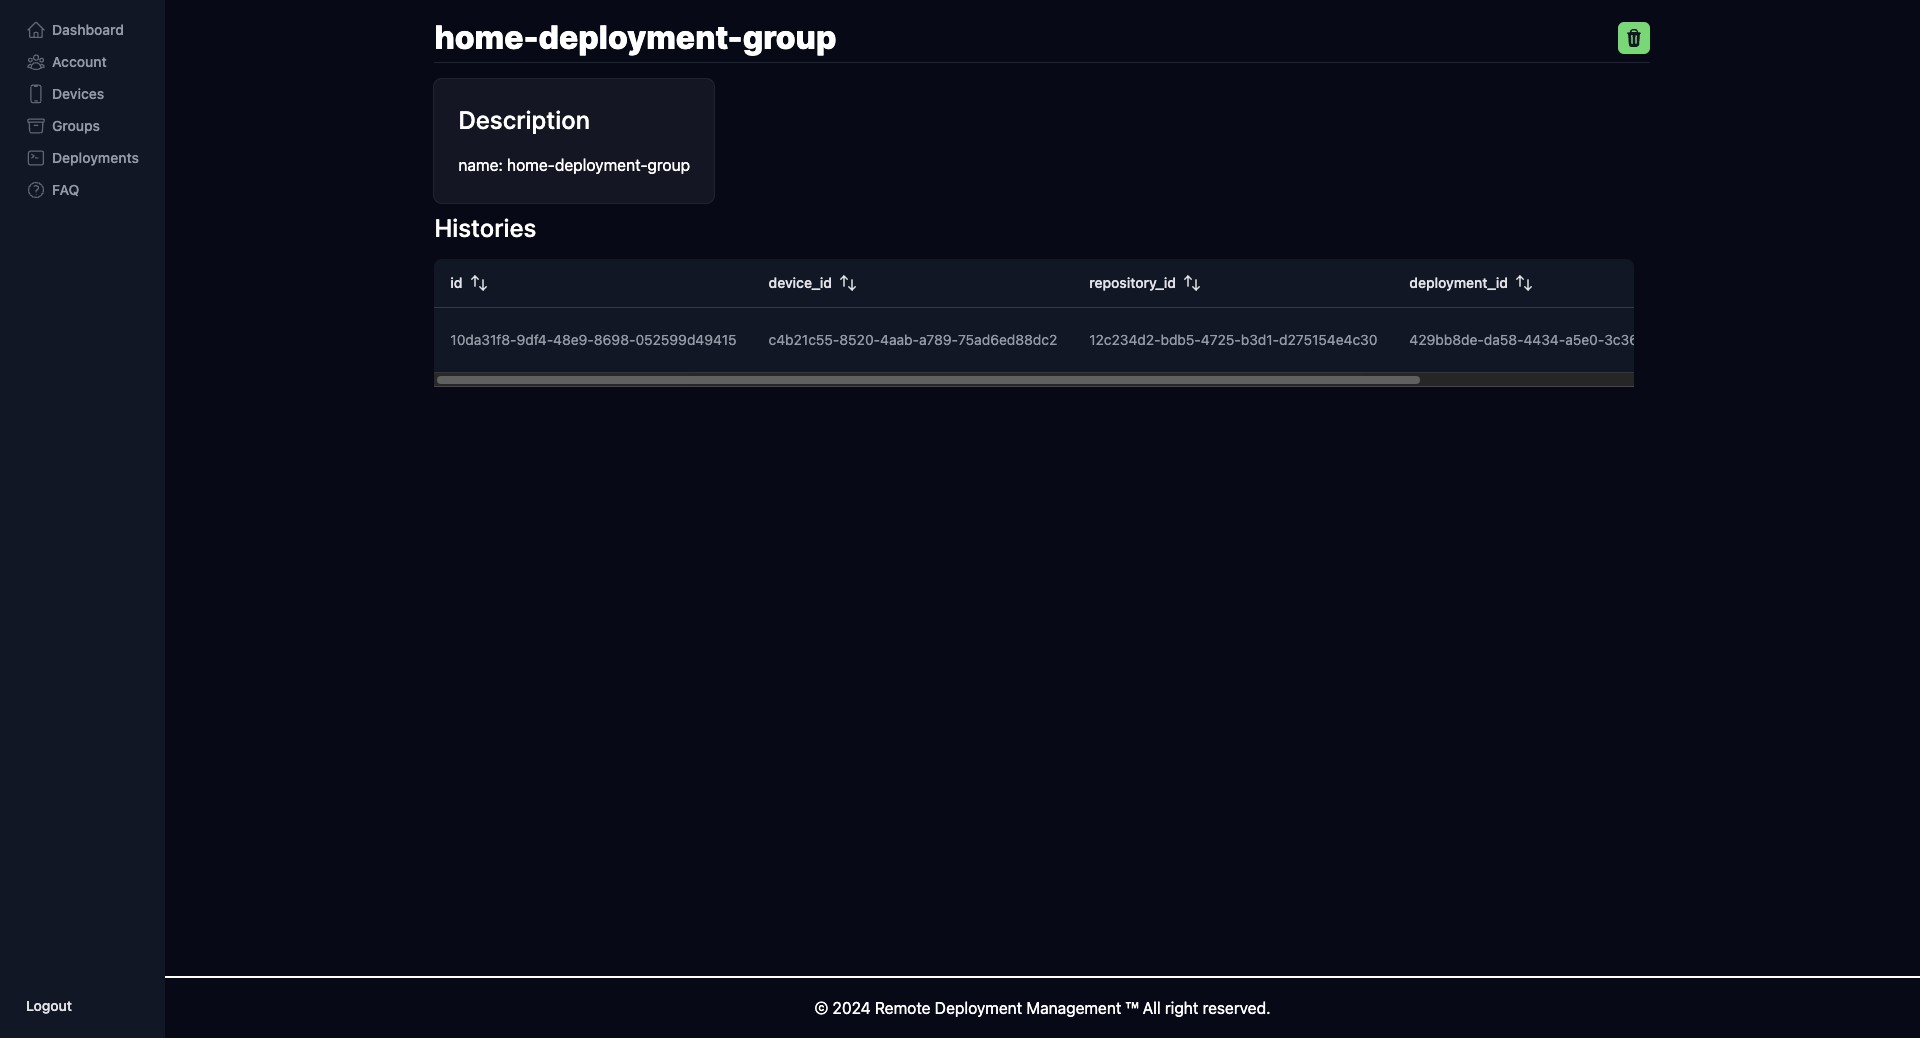
\includegraphics[width=1\textwidth]{resources/chapter-4/dashboard/deployment-detail-page.jpg}
  \caption{Halaman \textit{deployment detail}}
  \label{fig:halaman-deployment-detail}
\end{figure}

\begin{figure}[ht]
  \centering
  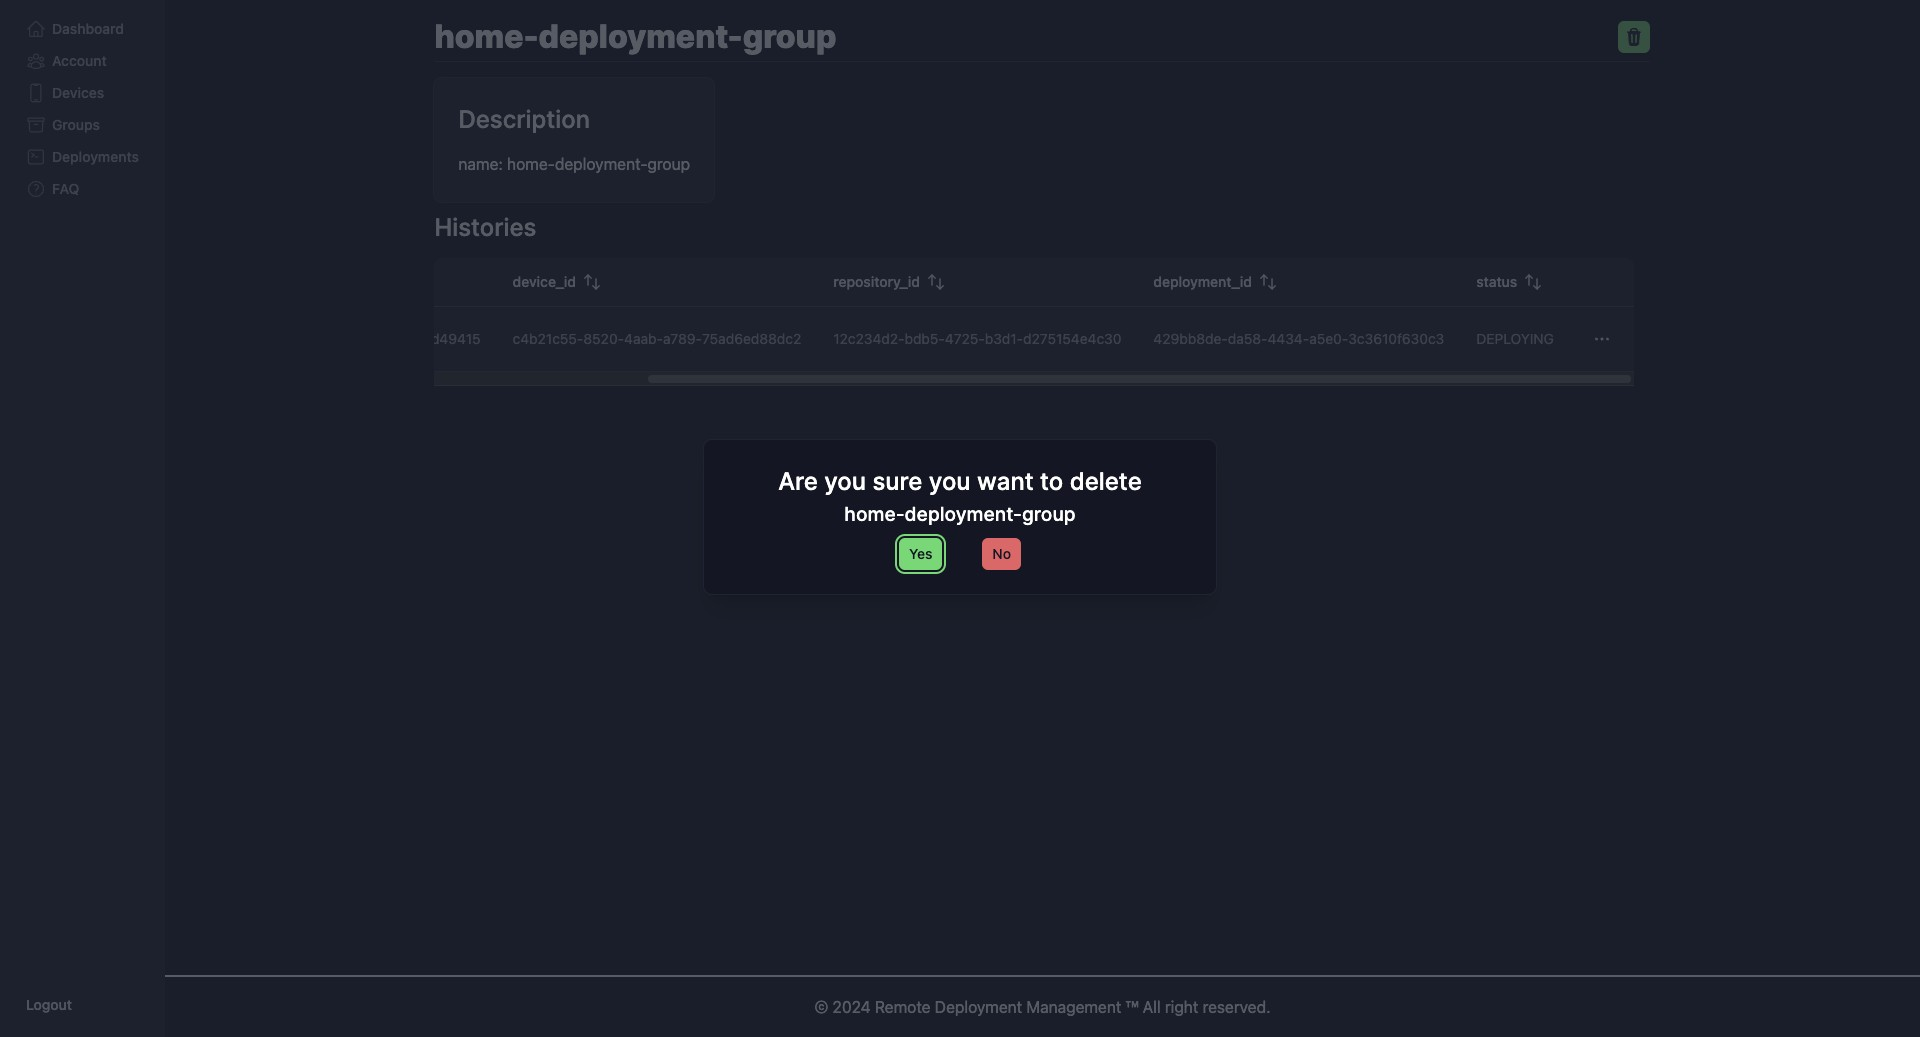
\includegraphics[width=1\textwidth]{resources/chapter-4/dashboard/deployment-detail-delete.jpg}
  \caption{Modal menghapus deployment pada halaman \textit{deployment detail}}
  \label{fig:halaman-deployment-detail-delete}
\end{figure}

\chapter{Pengujian}

\begin{figure}[ht]
  \centering
  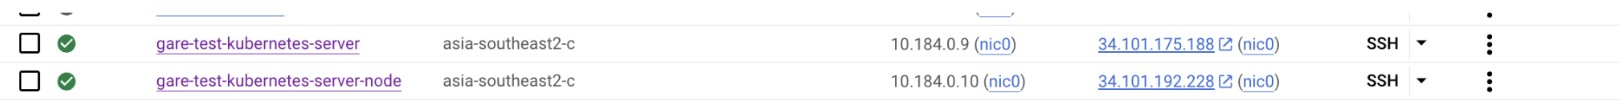
\includegraphics[width=0.8\textwidth]{resources/chapter-4/pengujian/kube-gcp-01.jpg}
  \caption{Hasil Pembuatan Virtual Machine pada GCP}
  \label{fig:hasil-pembuatan-virtual-machine-gcp}
\end{figure}

\begin{figure}[ht]
  \centering
  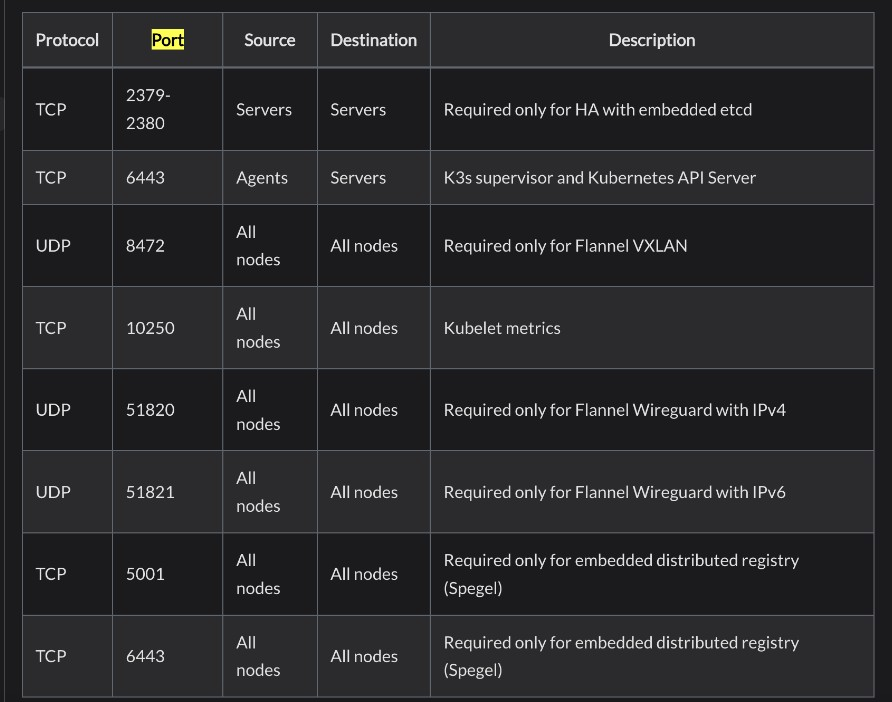
\includegraphics[width=0.8\textwidth]{resources/chapter-4/pengujian/kube-gcp-03.jpg}
  \caption{Daftar Kegunaan Port}
  \label{fig:daftar-kegunaan-port}
\end{figure}

\begin{figure}[ht]
  \centering
  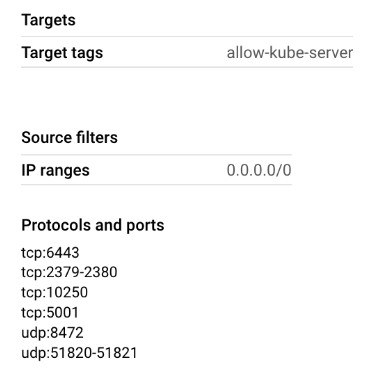
\includegraphics[width=0.8\textwidth]{resources/chapter-4/pengujian/kube-gcp-02.jpg}
  \caption{Hasil Firewall Rule pada GCP}
  \label{fig:hasil-firewall-rule-pada-gcp}
\end{figure}

\begin{figure}[ht]
  \centering
  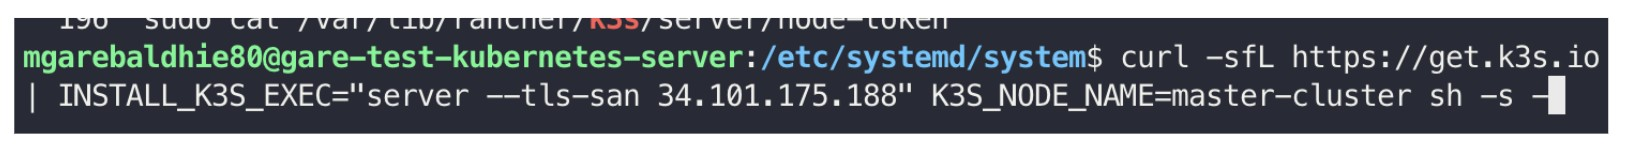
\includegraphics[width=0.8\textwidth]{resources/chapter-4/pengujian/kube-gcp-04.jpg}
  \caption{Instalasi Master Node di \textit{Virtual Machine}}
  \label{fig:instalasi-master-node-gcp}
\end{figure}

\begin{figure}[ht]
  \centering
  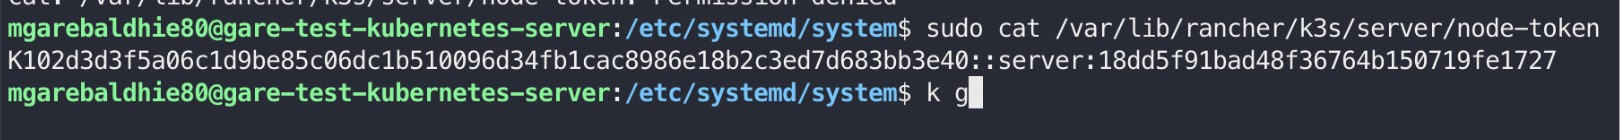
\includegraphics[width=0.8\textwidth]{resources/chapter-4/pengujian/kube-gcp-05.jpg}
  \caption{Pengambilan Token Registrasi Cluster}
  \label{fig:pengambilan-token-registrasi-cluster}
\end{figure}

\begin{figure}[ht]
  \centering
  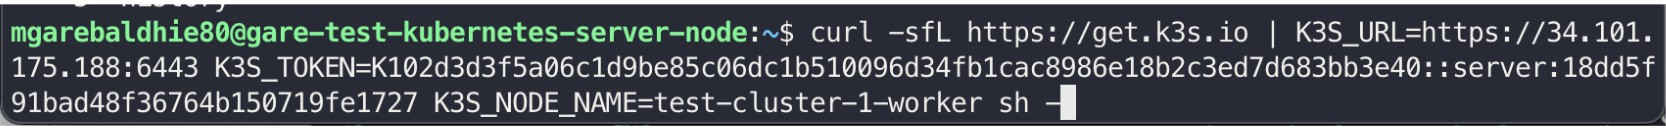
\includegraphics[width=0.8\textwidth]{resources/chapter-4/pengujian/kube-gcp-06.jpg}
  \caption{Instalasi Worker Node di \textit{Virtual Machine}}
  \label{fig:instalasi-worker-node-gcp}
\end{figure}

\begin{figure}[ht]
  \centering
  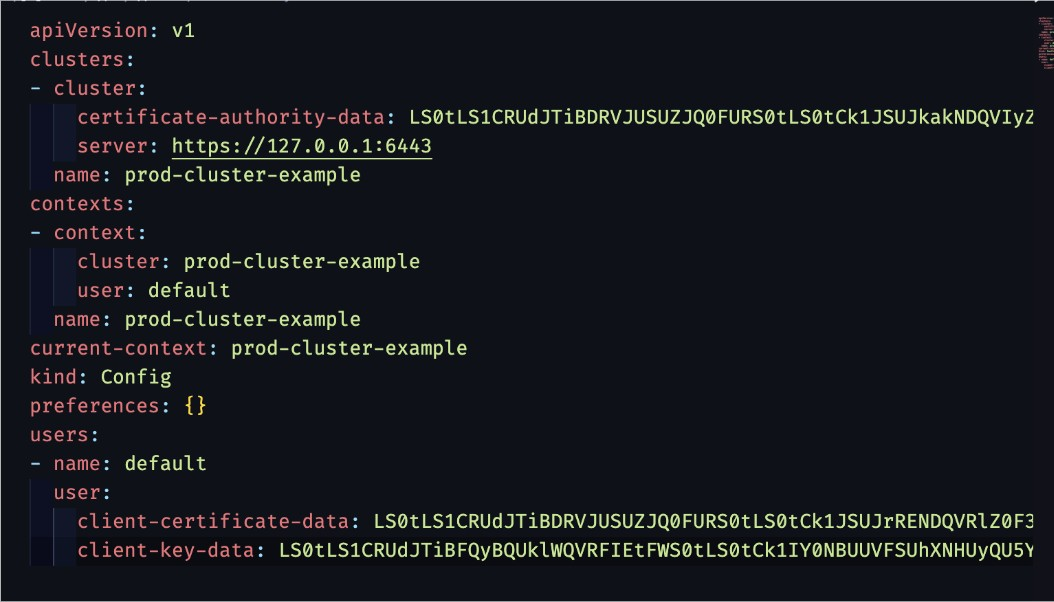
\includegraphics[width=0.8\textwidth]{resources/chapter-4/pengujian/kube-gcp-07.jpg}
  \caption{Konfigurasi \textit{Cluster} pada \textit{Master Node GCP}}
  \label{fig:konfigurasi-cluster-master-node-gcp}
\end{figure}

\begin{figure}[ht]
  \centering
  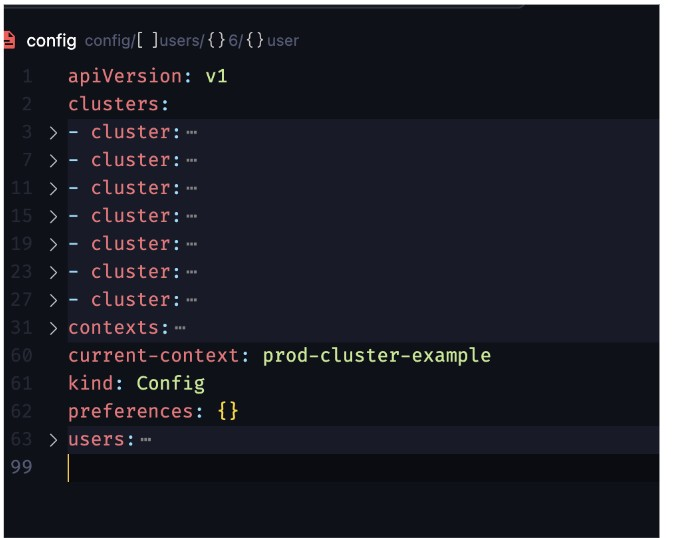
\includegraphics[width=0.8\textwidth]{resources/chapter-4/pengujian/kube-gcp-08.jpg}
  \caption{Pemindahan Konfigurasi \textit{Cluster} pada \textit{Master Node GCP}}
  \label{fig:proses-pemindahan-konfigurasi-master-gcp}
\end{figure}

\begin{figure}[ht]
  \centering
  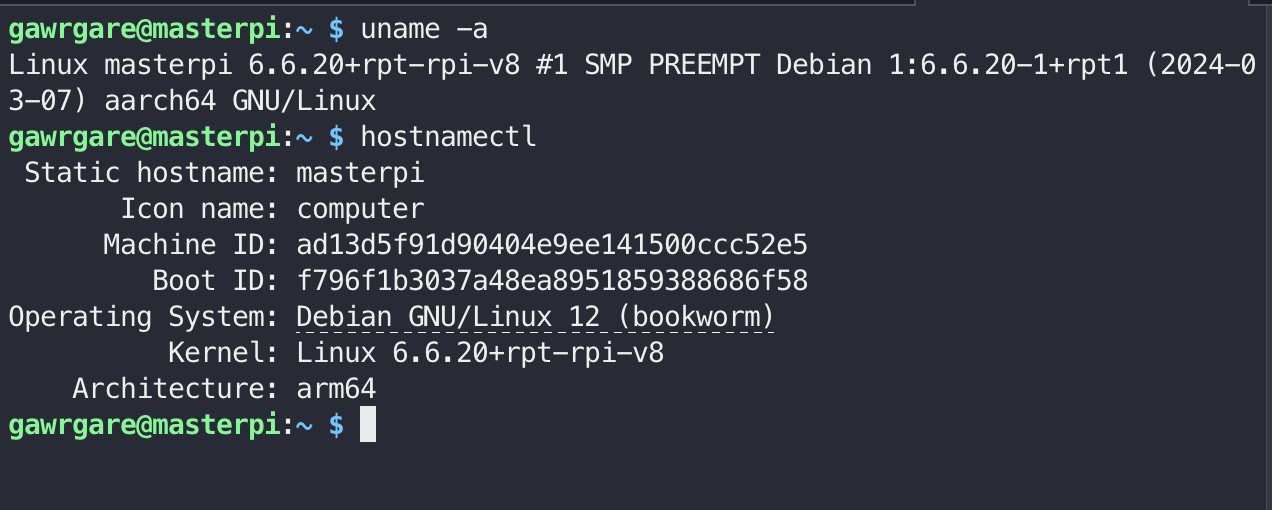
\includegraphics[width=0.8\textwidth]{resources/chapter-4/pengujian/raspi-01.jpg}
  \caption{Hostname Raspsi Master Nodes}
  \label{fig:hostname-raspi-master-nodes}
\end{figure}

\begin{figure}[ht]
  \centering
  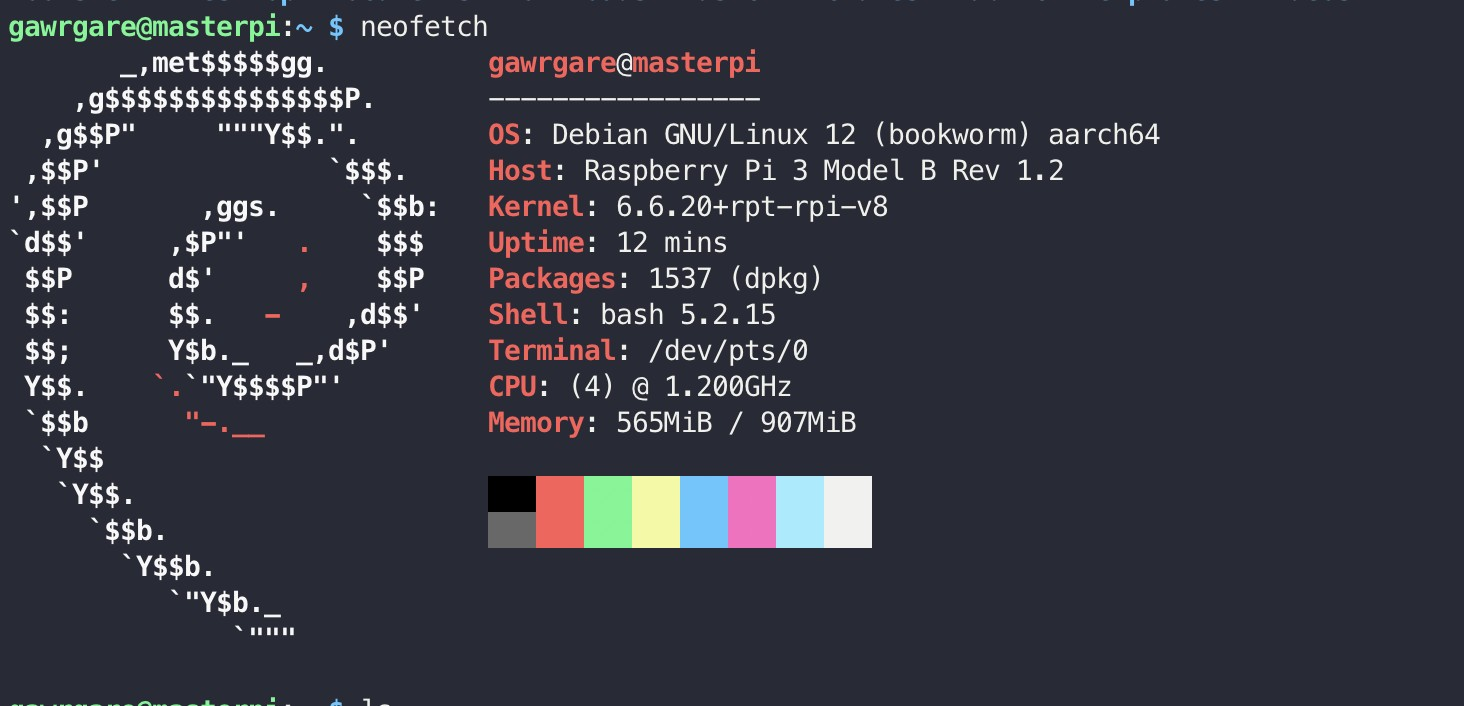
\includegraphics[width=0.8\textwidth]{resources/chapter-4/pengujian/raspi-master-neofetch.jpg}
  \caption{Spesifikasi Raspsi Master Nodes}
  \label{fig:spesifikasi-raspi-master-nodes}
\end{figure}

\begin{figure}[ht]
  \centering
  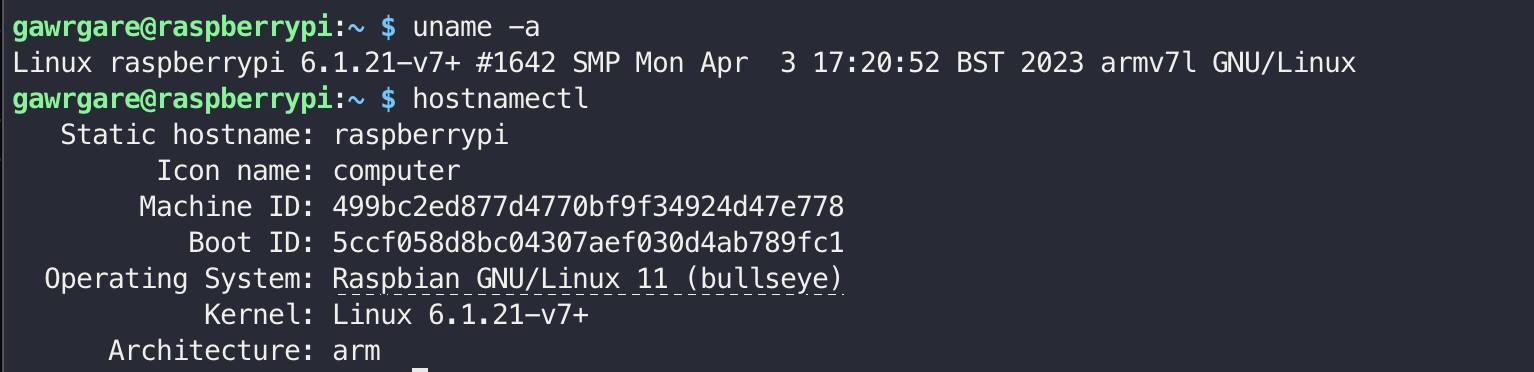
\includegraphics[width=0.8\textwidth]{resources/chapter-4/pengujian/raspi-01-worker.jpg}
  \caption{Hostname Raspsi Worker Nodes}
  \label{fig:hostname-raspi-worker-nodes}
\end{figure}

\begin{figure}[ht]
  \centering
  \includegraphics[width=0.8\textwidth]{resources/chapter-4/pengujian/raspi-worker-neofetch.jpg}
  \caption{Spesifikasi Raspsi Worker Nodes}
  \label{fig:spesifikasi-raspi-worker-nodes}
\end{figure}

\begin{figure}[ht]
  \centering
  \includegraphics[width=0.8\textwidth]{resources/chapter-4/pengujian/raspi-02-additional.jpg}
  \caption{\textit{Additional Command} untuk RaspberryPi}
  \label{fig:additional-command-raspberrypi}
\end{figure}

\begin{figure}[ht]
  \centering
  \includegraphics[width=0.8\textwidth]{resources/chapter-4/pengujian/raspi-02-additional-02.jpg}
  \caption{Penambahan \textit{cgroups} pada \textit{Cmdline}}
  \label{fig:penambahan-cgroups-pada-cmdline}
\end{figure}

\begin{figure}[ht]
  \centering
  \includegraphics[width=0.8\textwidth]{resources/chapter-4/pengujian/raspi-03.jpg}
  \caption{Instalasi Master Raspi \textit{Node}}
  \label{fig:instalasi-master-raspi-nodes}
\end{figure}

\begin{figure}[ht]
  \centering
  \includegraphics[width=0.8\textwidth]{resources/chapter-4/pengujian/raspi-token-gen.jpg}
  \caption{Master Raspi Generate Token}
  \label{fig:raspi-master-gen-token}
\end{figure}

\begin{figure}[ht]
  \centering
  \includegraphics[width=0.8\textwidth]{resources/chapter-4/pengujian/raspi-04.jpg}
  \caption{Instalasi Worker Raspi \textit{Node}}
  \label{fig:instalasi-worker-raspi-node}
\end{figure}

\begin{figure}[ht]
  \centering
  \includegraphics[width=0.8\textwidth]{resources/chapter-4/pengujian/raspi-kube-config.jpg}
  \caption{Kubernetes Config RaspberryPi}
  \label{fig:raspi-kube-config}
\end{figure}

\begin{figure}[ht]
  \centering
  \includegraphics[width=0.8\textwidth]{resources/chapter-4/pengujian/raspi-kube-config.jpg}
  \caption{Menambagkan Kubernetes Config RaspberryPi pada Sistem}
  \label{fig:raspi-add-kubeconfig}
\end{figure}

\begin{figure}[ht]
  \centering
  \includegraphics[width=0.8\textwidth]{resources/chapter-4/pengujian/pengujian-sistem-raspi-09-dockerfile.jpg}
  \caption{Python Docker LED Script}
  \label{fig:raspi-docker-led-script}
\end{figure}

\begin{figure}[ht]
  \centering
  \includegraphics[width=0.8\textwidth]{resources/chapter-4/pengujian/pengujian-sistem-raspi-01.jpg}
  \caption{Pembuatan \textit{Company} Raspi Company}
  \label{fig:pengujian-sistem-raspi-01}
\end{figure}

\begin{figure}[ht]
  \centering
  \includegraphics[width=0.8\textwidth]{resources/chapter-4/pengujian/pengujian-sistem-raspi-02.jpg}
  \caption{Pembuatan \textit{User} Raspi-User}
  \label{fig:pengujian-sistem-raspi-02}
\end{figure}

\begin{figure}[ht]
  \centering
  \includegraphics[width=0.8\textwidth]{resources/chapter-4/pengujian/pengujian-sistem-raspi-04-1.jpg}
  \caption{Pembuatan \textit{Device} Raspi}
  \label{fig:pengujian-sistem-raspi-04}
\end{figure}

\begin{figure}[ht]
  \centering
  \includegraphics[width=0.8\textwidth]{resources/chapter-4/pengujian/pengujian-sistem-raspi-05.jpg}
  \caption{Pembuatan \textit{Groups} Raspi}
  \label{fig:pengujian-sistem-raspi-05}
\end{figure}

\begin{figure}[ht]
  \centering
  \includegraphics[width=0.8\textwidth]{resources/chapter-4/pengujian/pengujian-sistem-raspi-layout.jpg}
  \caption{Layout Sederhana \textit{Clustser} RaspberryPi}
  \label{fig:pengujian-sistem-raspi-layout}
\end{figure}

\begin{figure}[ht]
  \centering
  \includegraphics[width=0.8\textwidth]{resources/chapter-4/pengujian/pengujian-sistem-raspi-hasil-a.jpg}
  \caption{Hasil Pengujian Sistem Target Deployment Raspi}
  \label{fig:hasil-pengujian-sistem-raspi-target}
\end{figure}

\begin{figure}[ht]
  \centering
  \includegraphics[width=0.8\textwidth]{resources/chapter-4/pengujian/pengujian-sistem-raspi-hasil-b.jpg}
  \caption{Hasil Pengujian Sistem Custom Deployment Raspi}
  \label{fig:hasil-pengujian-sistem-raspi-custom}
\end{figure}

\begin{figure}[ht]
  \centering
  \includegraphics[width=0.8\textwidth]{resources/chapter-4/pengujian/p00.jpg}
  \caption{Daftar Nama Cluster yang Tersedia pada Service}
  \label{fig:list-cluster-tersedia}
\end{figure}




\chapter{Pengujian Sistem RaspberryPi}

\begin{figure}[ht]
  \centering
  \includegraphics[width=0.8\textwidth]{resources/chapter-4/pengujian/pengujian-sistem-raspi-09-dockerfile.jpg}
  \caption{Python Docker LED Script}
  \label{fig:raspi-docker-led-script}
\end{figure}

\begin{figure}[ht]
  \centering
  \includegraphics[width=0.8\textwidth]{resources/chapter-4/pengujian/pengujian-sistem-raspi-01.jpg}
  \caption{Pembuatan \textit{Company} Raspi Company}
  \label{fig:pengujian-sistem-raspi-01}
\end{figure}

\begin{figure}[ht]
  \centering
  \includegraphics[width=0.8\textwidth]{resources/chapter-4/pengujian/pengujian-sistem-raspi-02.jpg}
  \caption{Pembuatan \textit{User} Raspi-User}
  \label{fig:pengujian-sistem-raspi-02}
\end{figure}

\begin{figure}[ht]
  \centering
  \includegraphics[width=0.8\textwidth]{resources/chapter-4/pengujian/pengujian-sistem-raspi-04-1.jpg}
  \caption{Pembuatan \textit{Device} Raspi}
  \label{fig:pengujian-sistem-raspi-04}
\end{figure}

\begin{figure}[ht]
  \centering
  \includegraphics[width=0.8\textwidth]{resources/chapter-4/pengujian/pengujian-sistem-raspi-05.jpg}
  \caption{Pembuatan \textit{Groups} Raspi}
  \label{fig:pengujian-sistem-raspi-05}
\end{figure}

\begin{figure}[ht]
  \centering
  \includegraphics[width=0.8\textwidth]{resources/chapter-4/pengujian/pengujian-sistem-raspi-10.jpg}
  \caption{Riwayat \textit{deployment} "raspi-deployment-bink"}
  \label{fig:pengujian-sistem-raspi-10}
\end{figure}

\begin{figure}[ht]
  \centering
  \includegraphics[width=0.8\textwidth]{resources/chapter-4/pengujian/pengujian-sistem-raspi-layout.jpg}
  \caption{Layout Sederhana \textit{Clustser} RaspberryPi}
  \label{fig:pengujian-sistem-raspi-layout}
\end{figure}

\begin{figure}[ht]
  \centering
  \includegraphics[width=0.8\textwidth]{resources/chapter-4/pengujian/pengujian-sistem-raspi-hasil-a.jpg}
  \caption{Hasil Pengujian Sistem Target Deployment Raspi}
  \label{fig:hasil-pengujian-sistem-raspi-target}
\end{figure}

\begin{figure}[ht]
  \centering
  \includegraphics[width=0.8\textwidth]{resources/chapter-4/pengujian/pengujian-sistem-raspi-hasil-b.jpg}
  \caption{Hasil Pengujian Sistem Custom Deployment Raspi}
  \label{fig:hasil-pengujian-sistem-raspi-custom}
\end{figure}

\bgroup
\begin{table}[ht]
  \def\arraystretch{1.3}
  \caption{Skenario dan Hasil Pengujian Sistem \textit{RaspberryPi}}
  \label{tab:pengujian-sistem-raspi}
  \centering
  \begin{tabular}{|p{2cm}|p{2cm}|p{4cm}|p{3cm}|p{2cm}|}
    \hline
    \centering{ID Fungsional} & \centering{ID Pengujian}                            & \centering{Skenario}                                                                           & \centering{Ekspektasi}                                                                    & Realita \\
    \hline
    F01                       & P20                                                 & \textit{Admin} membuat \textit{company} yang dengan nama "raspi-company"                       & \textit{Admin} berhasil mendaftarkan \textit{company}                                     & Sesuai  \\
    \hline
    F04                       & P21                                                 & \textit{Admin} membuat \textit{user} yang dengan email "raspi@gmail.com"                       & \textit{Admin} berhasil mendaftarkan \textit{user}                                        & Sesuai  \\
    \hline
    F06                       & P22                                                 & \textit{User} ingin login dengan kredensial "raspi@gmail.com"                                  & \textit{User} berhasil login ke dalam sistem                                              & Sesuai  \\
    \hline
    F10                       & P23                                                 & \textit{User} mendaftarkan dua \textit{devices} dengan nama "raspi-master" dan
    raspi-worker"             & \textit{User} berhasil mendaftarkan \textit{device} & Sesuai                                                                                                                                                                                               \\
    \hline
    F13                       & P24                                                 & \textit{User} mendaftarkan \textit{group} dengan nama "raspi-group-blink"                      & \textit{User} berhasil mendaftarkan \textit{group}                                        & Sesuai  \\
    \hline
    F16                       & P25                                                 & \textit{User} mendaftarkan \textit{device} pada \textit{group} dengan nama "raspi-group-blink" & \textit{User} berhasil mendaftarkan \textit{device} ke \textit{group} "raspi-group-blink" & Sesuai  \\
    \hline
    F17                       & P26                                                 & \textit{User} mendaftarkan \textit{deployment images} dengan nama "raspi-image-blink"          & \textit{User} berhasil mendaftarkan \textit{deployment images}                            & Sesuai  \\
    \hline
  \end{tabular}
\end{table}
\egroup

\bgroup
\begin{table}[ht]
  \def\arraystretch{1.3}
  \centering
  \begin{tabular}{|p{2cm}|p{2cm}|p{4cm}|p{3cm}|p{2cm}|}
    \hline
    \centering{ID Fungsional} & \centering{ID Pengujian} & \centering{Skenario}                                                                                                                                                                                                                  & \centering{Ekspektasi}                                                 & Realita \\
    \hline

    F18                       & P27                      & \textit{User} melihat daftar \textit{deployment images} yang tersedia dengan mengunjungi halaman /deployments                                                                                                                         & \textit{User} berhasil melihat daftar \textit{deployment images}       & Sesuai  \\
    \hline
    F20                       & P28                      & \textit{User} membuat \textit{deployment plan} dengan nama "raspi-deployment-blink"                                                                                                                                                   & \textit{User} berhasil membuat \textit{deployment plan}                & Sesuai  \\
    \hline
    F21                       & P29                      & \textit{User} melihat daftar \textit{deployment plan} yang tersedia dengan mengunjungi halaman /deployments                                                                                                                           & \textit{User} berhasil melihat daftar \textit{deployment plan}         & Sesuai  \\
    \hline
    F23                       & P30                      & \textit{User} melakukan \textit{remote deployment} dengan menggunakan \textit{deployment plan} "raspi-deployment-blink" dengan dua tipe \textit{deployment} yaitu \textit{targeted} dan \textit{custom} dengan tujuan \textit{groups} & \textit{User} berhasil melakukan \textit{remote deployment}            & Sesuai  \\
    \hline
    F24                       & P31                      & \textit{User} ingin melihat riwayat deployment dari "raspi-blink-deployment"                                                               dengan menekan tombol elipsis dan tombol detail pada tabel                                 & \textit{User} berhasil melihat riwayat \textit{deployment} yang sesuai & Sesuai  \\
    \hline
  \end{tabular}
\end{table}
\egroup

\chapter{Pengujian Sistem GCP}

\begin{figure}[ht]
  \centering
  \includegraphics[width=0.8\textwidth]{resources/chapter-4/pengujian/pengujian-sistem-gcp-01.jpg}
  \caption{Pembuatan \textit{Company} pada Cluster \textit{GCP}}
  \label{fig:pengujian-sistem-gcp-01}
\end{figure}

\begin{figure}[ht]
  \centering
  \includegraphics[width=0.8\textwidth]{resources/chapter-4/pengujian/pengujian-sistem-gcp-02.jpg}
  \caption{Pembuatan \textit{User} pada Cluster \textit{GCP}}
  \label{fig:pengujian-sistem-gcp-02}
\end{figure}

\begin{figure}[ht]
  \centering
  \includegraphics[width=0.8\textwidth]{resources/chapter-4/pengujian/pengujian-sistem-gcp-03.jpg}
  \caption{\textit{User} Sukses Melakukan Login}
  \label{fig:pengujian-sistem-gcp-03}
\end{figure}

\begin{figure}[ht]
  \centering
  \includegraphics[width=0.8\textwidth]{resources/chapter-4/pengujian/pengujian-sistem-gcp-04.jpg}
  \caption{Pembuatan \textit{Device} pada \textit{Cluster GCP}}
  \label{fig:pengujian-sistem-gcp-04}
\end{figure}

\begin{figure}[ht]
  \centering
  \includegraphics[width=0.8\textwidth]{resources/chapter-4/pengujian/pengujian-sistem-gcp-05.jpg}
  \caption{Pembuatan \textit{Deployment Plan} pada \textit{Cluster GCP}}
  \label{fig:pengujian-sistem-gcp-05}
\end{figure}

\begin{figure}[ht]
  \centering
  \includegraphics[width=0.8\textwidth]{resources/chapter-4/pengujian/pengujian-sistem-gcp-06.jpg}
  \caption{Hasil \textit{Remote Deployment} pada \textit{Cluster GCP}}
  \label{fig:pengujian-sistem-gcp-06}
\end{figure}

\begin{figure}[ht]
  \centering
  \includegraphics[width=0.8\textwidth]{resources/chapter-4/pengujian/pengujian-sistem-gcp-07.jpg}
  \caption{Hasil Penghapusan \textit{Remote Deployment} pada \textit{Cluster GCP}}
  \label{fig:pengujian-sistem-gcp-07}
\end{figure}

\begin{figure}[ht]
  \centering
  \includegraphics[width=0.8\textwidth]{resources/chapter-4/pengujian/pengujian-sistem-gcp-08.jpg}
  \caption{Hasil Penghapusan \textit{Deployment Plan} pada \textit{Cluster GCP}}
  \label{fig:pengujian-sistem-gcp-08}
\end{figure}

\begin{figure}[ht]
  \centering
  \includegraphics[width=0.8\textwidth]{resources/chapter-4/pengujian/pengujian-sistem-gcp-09.jpg}
  \caption{Hasil Penghapusan \textit{Deployment Images} pada \textit{Cluster GCP}}
  \label{fig:pengujian-sistem-gcp-09}
\end{figure}

\bgroup
\begin{table}[ht]
  \def\arraystretch{1.3}
  \caption{Skenario dan Hasil Pengujian Sistem pada \textit{Cluster GCP}}
  \label{tab:pengujian-sistem-gcp}
  \centering
  \begin{tabular}{|p{2cm}|p{2cm}|p{4cm}|p{3cm}|p{2cm}|}
    \hline
    \centering{ID Fungsional} & \centering{ID Pengujian} & \centering{Skenario}                                                                                        & \centering{Ekspektasi}                                & Realita \\
    \hline
    F01                       & P32                      & \textit{Admin} membuat \textit{company} yang dengan nama "test-semhas"                                      & \textit{Admin} berhasil mendaftarkan \textit{company} & Sesuai  \\
    \hline
    F04                       & P33                      & \textit{Admin} membuat \textit{user} yang dengan email "test@gmail.com"                                     & \textit{Admin} berhasil mendaftarkan \textit{user}    & Sesuai  \\
    \hline
    F06                       & P34                      & \textit{User} ingin login dengan kredensial "test@gmail.com"                                                & \textit{User} berhasil login ke dalam sistem          & Sesuai  \\
    \hline
    F10                       & P35                      & \textit{User} mendaftarkan \textit{device} dengan nama "raspberrypi-pi-1" dengan nama node "master-cluster" & \textit{User} berhasil mendaftarkan \textit{device}   & Sesuai  \\
    \hline
  \end{tabular}
\end{table}
\egroup

\bgroup
\begin{table}[ht]
  \def\arraystretch{1.3}
  \centering
  \begin{tabular}{|p{2cm}|p{2cm}|p{4cm}|p{3cm}|p{2cm}|}
    \hline
    \centering{ID Fungsional} & \centering{ID Pengujian} & \centering{Skenario}                                                                                          & \centering{Ekspektasi}                                            & Realita \\
    \hline

    F18                       & P36                      & \textit{User} melihat daftar \textit{deployment images} yang tersedia dengan mengunjungi halaman /deployments & \textit{User} berhasil melihat daftar \textit{deployment images}  & Sesuai  \\
    \hline
    F20                       & P37                      & \textit{User} membuat \textit{deployment plan} dengan nama "deploy-nginx-to-system"                           & \textit{User} berhasil membuat \textit{deployment plan}           & Sesuai  \\
    \hline
    F22                       & P38                      & \textit{User} menghapus \textit{deployment plan} dengan nama "deploy-nginx-to-system"                         & \textit{User} berhasil melihat menghapus \textit{deployment plan} & Sesuai  \\
    \hline
    F19                       & P39                      & \textit{User} menghapus \textit{deployment images} dengan nama NGINX                                          & \textit{User} berhasil menghapus \textit{deployment images}       & Sesuai  \\
    \hline
  \end{tabular}
\end{table}
\egroup

\chapter{Tabel Pengujian}

\bgroup
\begin{table}[ht]
  \def\arraystretch{1.5}
  \caption{Skenario dan Hasil Pengujian Domain \textit{Company}}
  \label{tab:pengujian-domain-company}
  \centering
  \begin{tabular}{|p{2cm}|p{2cm}|p{3cm}|p{3cm}|p{1.5cm}|}
    \hline
    \centering{ID Fungsional} & \centering{ID Pengujian} & \centering{Skenario}                                                                 & \centering{Ekspektasi}                                                                             & Realita \\
    \hline
    F01                       & P01                      & Admin mendaftarkan \textit{company} dengan cluster name yang tersedia                & Admin berhasil mendaftarkan \textit{company}                                                       & Sesuai  \\
    \hline
    F01                       & P02                      & Admin mendaftarkan \textit{company} dengan cluster name yang tidak valid             & Admin tidak berhasil mendaftarkan karena cluster name tidak valid                                  & Sesuai  \\
    \hline
    F02                       & P03                      & Admin membuat \textit{request} untuk melihat seluruh \textit{company} pada sistem    & Admin dapat melihat seluruh \textit{company} pada sistem                                           & Sesuai  \\
    \hline
    F03                       & P04                      & Admin melakukan DELETE \textit{request} untuk menghapus \textit{company} pada sistem & Admin dapat menghapus \textit{company} pada sistem dengan memberikan id company yang ingin dihapus & Sesuai  \\
    \hline
  \end{tabular}
\end{table}
\egroup


\bgroup
\begin{table}[ht]
  \def\arraystretch{1.3}
  \caption{Skenario dan Hasil Pengujian Domain \textit{User}}
  \label{tab:pengujian-domain-user}
  \centering
  \begin{tabular}{|p{2cm}|p{2cm}|p{3cm}|p{3cm}|p{1.5cm}|}
    \hline
    \centering{ID Fungsional} & \centering{ID Pengujian} & \centering{Skenario}                                                                           & \centering{Ekspektasi}                                                                                    & Realita \\
    \hline
    F04                       & P05                      & Admin mendaftarkan \textit{user} dengan kredensial yang valid                                  & Admin berhasil mendaftarkan \textit{user}                                                                 & Sesuai  \\
    \hline
    F05                       & P06                      & Admin menghapus \textit{user} dengan id yang valid                                             & Admin berhasil menghapus \textit{user} dari database                                                      & Sesuai  \\
    \hline
    F06                       & P07                      & \textit{User} ingin login ke dalam sistem dengan memasukan kredensial yang valid               & User berhasil login ke dalam sistem                                                                       & Sesuai  \\
    \hline
    F06                       & P08                      & \textit{User} ingin login ke dalam sistem dengan memasukan kredensial yang tidak valid         & User tidak berhasil login ke dalam sistem                                                                 & Sesuai  \\
    \hline
    F07                       & P09                      & \textit{User} ingin melakukan logout dari sistem                                               & \textit{User} berhasil melakukan logout dengan menekan tombol \textit{logout} pada \textit{sidebar}       & Sesuai  \\
    \hline
    F08                       & P10                      & \textit{User} mendapatkan informasi mengenai detail \textit{company} perusahaan yang ia masuki & {User} berhasil mendapatkan informasi detail \textit{company} dengan cara mengunjungi halaman /account    & Sesuai  \\
    \hline
    F09                       & P11                      & \textit{User} mendaptkan daftar \textit{user} lain pada \textit{company} yang sama.            & \textit{User} berhasil mendapatkan informasi datar \textit{user} dengan cara mengunjungi halaman /account & Sesuai  \\
    \hline
  \end{tabular}
\end{table}
\egroup

\bgroup
\begin{table}[ht]
  \def\arraystretch{1.3}
  \caption{Skenario dan Hasil Pengujian Domain \textit{Device}}
  \label{tab:pengujian-domain-device}
  \centering
  \begin{tabular}{|p{2cm}|p{2cm}|p{3cm}|p{3cm}|p{1.5cm}|}
    \hline
    \centering{ID Fungsional} & \centering{ID Pengujian} & \centering{Skenario}                                                                                 & \centering{Ekspektasi}                                                    & Realita \\
    \hline
    F10                       & P12                      & \textit{User} membuat \textit{device} yang valid                                                     & \textit{User} berhasil mendaftarkan \textit{device} kepada sistem         & Sesuai  \\
    \hline
    F10                       & P13                      & {User} membuat \textit{device} yang tidak valid                                                      & \textit{User} gagal mendaftarkan \textit{device} kepada sistem            & Sesuai  \\
    \hline
    F11                       & P14                      & \textit{User} ingin melihat daftar \textit{device} yang tersedia dengan mengunjungi halaman /devices & User berhasil melihat daftar \textit{device} yang tersedia                & Sesuai  \\
    \hline
    F12                       & P15                      & \textit{User} ingin menghapus salah satu \textit{device} yang dimiliki                               & \textit{User} berhasil untuk menghapus \textit{device} yang ingin dihapus & Sesuai  \\
    \hline
  \end{tabular}
\end{table}
\egroup


\bgroup
\begin{table}[ht]
  \def\arraystretch{1.3}
  \caption{Skenario dan Hasil Pengujian Domain \textit{Groups}}
  \label{tab:pengujian-domain-groups}
  \centering
  \begin{tabular}{|p{2cm}|p{2cm}|p{3cm}|p{3cm}|p{1.5cm}|}
    \hline
    \centering{ID Fungsional} & \centering{ID Pengujian} & \centering{Skenario}                                                                               & \centering{Ekspektasi}                                                   & Realita \\
    \hline
    F13                       & P16                      & \textit{User} membuat \textit{group} yang dengan nama "group-baru"                                 & \textit{User} berhasil mendaftarkan \textit{group} kepada sistem         & Sesuai  \\
    \hline
    F13                       & P17                      & {User} membuat \textit{group} yang memiliki nama duplikat yaitu "group-baru"                       & \textit{User} gagal mendaftarkan \textit{group} kepada sistem            & Sesuai  \\
    \hline
    F14                       & P18                      & \textit{User} ingin melihat daftar \textit{group} yang tersedia dengan mengunjungi halaman /groups & User berhasil melihat daftar \textit{group} yang tersedia                & Sesuai  \\
    \hline
    F15                       & P19                      & \textit{User} ingin menghapus salah satu \textit{group} yang dimiliki                              & \textit{User} berhasil untuk menghapus \textit{group} yang ingin dihapus & Sesuai  \\
    \hline
  \end{tabular}
\end{table}
\egroup

\bgroup
\begin{table}[ht]
  \def\arraystretch{1.3}
  \caption{Skenario dan Hasil Pengujian Sistem \textit{RaspberryPi}}
  \label{tab:pengujian-sistem-raspi}
  \centering
  \begin{tabular}{|p{2cm}|p{2cm}|p{3cm}|p{3cm}|p{1.5cm}|}
    \hline
    \centering{ID Fungsional} & \centering{ID Pengujian}                            & \centering{Skenario}                                                                           & \centering{Ekspektasi}                                                                    & Realita \\
    \hline
    F01                       & P20                                                 & \textit{Admin} membuat \textit{company} yang dengan nama "raspi-company"                       & \textit{Admin} berhasil mendaftarkan \textit{company}                                     & Sesuai  \\
    \hline
    F04                       & P21                                                 & \textit{Admin} membuat \textit{user} yang dengan email "raspi@gmail.com"                       & \textit{Admin} berhasil mendaftarkan \textit{user}                                        & Sesuai  \\
    \hline
    F06                       & P22                                                 & \textit{User} ingin login dengan kredensial "raspi@gmail.com"                                  & \textit{User} berhasil login ke dalam sistem                                              & Sesuai  \\
    \hline
    F10                       & P23                                                 & \textit{User} mendaftarkan dua \textit{devices} dengan nama "raspi-master" dan
    raspi-worker"             & \textit{User} berhasil mendaftarkan \textit{device} & Sesuai                                                                                                                                                                                               \\
    \hline
    F13                       & P24                                                 & \textit{User} mendaftarkan \textit{group} dengan nama "raspi-group-blink"                      & \textit{User} berhasil mendaftarkan \textit{group}                                        & Sesuai  \\
    \hline
    F16                       & P25                                                 & \textit{User} mendaftarkan \textit{device} pada \textit{group} dengan nama "raspi-group-blink" & \textit{User} berhasil mendaftarkan \textit{device} ke \textit{group} "raspi-group-blink" & Sesuai  \\
    \hline
    F17                       & P26                                                 & \textit{User} mendaftarkan \textit{deployment images} dengan nama "raspi-image-blink"          & \textit{User} berhasil mendaftarkan \textit{deployment images}                            & Sesuai  \\
    \hline
  \end{tabular}
\end{table}
\egroup

\bgroup
\begin{table}[ht]
  \def\arraystretch{1.3}
  \centering
  \begin{tabular}{|p{2cm}|p{2cm}|p{3cm}|p{3cm}|p{1.5cm}|}
    \hline
    \centering{ID Fungsional} & \centering{ID Pengujian} & \centering{Skenario}                                                                                                                                                                                                                  & \centering{Ekspektasi}                                                 & Realita \\
    \hline

    F18                       & P27                      & \textit{User} melihat daftar \textit{deployment images} yang tersedia dengan mengunjungi halaman /deployments                                                                                                                         & \textit{User} berhasil melihat daftar \textit{deployment images}       & Sesuai  \\
    \hline
    F20                       & P28                      & \textit{User} membuat \textit{deployment plan} dengan nama "raspi-deployment-blink"                                                                                                                                                   & \textit{User} berhasil membuat \textit{deployment plan}                & Sesuai  \\
    \hline
    F21                       & P29                      & \textit{User} melihat daftar \textit{deployment plan} yang tersedia dengan mengunjungi halaman /deployments                                                                                                                           & \textit{User} berhasil melihat daftar \textit{deployment plan}         & Sesuai  \\
    \hline
    F23                       & P30                      & \textit{User} melakukan \textit{remote deployment} dengan menggunakan \textit{deployment plan} "raspi-deployment-blink" dengan dua tipe \textit{deployment} yaitu \textit{targeted} dan \textit{custom} dengan tujuan \textit{groups} & \textit{User} berhasil melakukan \textit{remote deployment}            & Sesuai  \\
    \hline
    F24                       & P31                      & \textit{User} ingin melihat riwayat deployment dari "raspi-blink-deployment"                                                               dengan menekan tombol elipsis dan tombol detail pada tabel                                 & \textit{User} berhasil melihat riwayat \textit{deployment} yang sesuai & Sesuai  \\
    \hline
  \end{tabular}
\end{table}
\egroup

\bgroup
\begin{table}[ht]
  \def\arraystretch{1.3}
  \caption{Skenario dan Hasil Pengujian Sistem pada \textit{Cluster GCP}}
  \label{tab:pengujian-sistem-gcp}
  \centering
  \begin{tabular}{|p{2cm}|p{2cm}|p{3cm}|p{3cm}|p{1.5cm}|}
    \hline
    \centering{ID Fungsional} & \centering{ID Pengujian} & \centering{Skenario}                                                                                          & \centering{Ekspektasi}                                                 & Realita \\
    \hline
    F01                       & P32                      & \textit{Admin} membuat \textit{company} yang dengan nama "test-semhas"                                        & \textit{Admin} berhasil mendaftarkan \textit{company}                  & Sesuai  \\
    \hline
    F04                       & P33                      & \textit{Admin} membuat \textit{user} yang dengan email yaitu "test@gmail.com"                                 & \textit{Admin} berhasil membuat \textit{user} dengan email yang sesuai & Sesuai  \\
    \hline
    F06                       & P34                      & \textit{User} melakukan login dengan email yaitu "test@gmail.com"                                             & \textit{User} berhasil login                                           & Sesuai  \\
    \hline
    F10                       & P35                      & \textit{User} mendaftarkan \textit{device} dengan nama "raspberrypi-pi-1" dengan nama node "master-cluster"   & \textit{User} berhasil mendaftarkan \textit{device}                    & Sesuai  \\
    \hline
    F18                       & P36                      & \textit{User} melihat daftar \textit{deployment images} yang tersedia dengan mengunjungi halaman /deployments & \textit{User} berhasil melihat daftar \textit{deployment images}       & Sesuai  \\
    \hline
    F20                       & P37                      & \textit{User} membuat \textit{deployment plan} dengan nama "deploy-nginx-to-system"                           & \textit{User} berhasil membuat \textit{deployment plan}                & Sesuai  \\
    \hline
    F22                       & P38                      & \textit{User} menghapus \textit{deployment plan} dengan nama "deploy-nginx-to-system"                         & \textit{User} berhasil melihat menghapus \textit{deployment plan}      & Sesuai  \\
    \hline
    F19                       & P39                      & \textit{User} menghapus \textit{deployment images} dengan nama NGINX                                          & \textit{User} berhasil menghapus \textit{deployment images}            & Sesuai  \\
    \hline
  \end{tabular}
\end{table}
\egroup

\end{document}
